\documentclass[a4paper,12pt]{article}
\usepackage[utf8]{inputenc}
\usepackage{pgfplots}
\usepackage[hidelinks]{hyperref}
\usepackage[left=2cm,top=2cm,right=2cm,bottom=2cm]{geometry}
\usepackage{amsmath,amssymb}

%opening
\title{Autonomous Agents - Assignment 3 Report}
\author{Nicolò Girardi, Jorge Sáez Gómez, Johan Sundin}

\begin{document}

\maketitle

\section{Introduction}

In this assignment we worked on a predator versus prey grid world scenario, in which both the predator and the prey are learning agents \cite{Assignment}. There are small changes made to the grid world scenario compared to previous assignments. Unlike previous assignments, the prey is now also a learning agent. In addition, the environment is extended so that it can contain more than one predator. A terminal state is now defined as any state in which any two or more agents in the environment (predator or prey) occupy the same square in the grid.

Predators must work together in this scenario to catch the prey. If any predator catches the prey, all predators receive a reward of +10. The prey receives a reward of -10 in this case. However, if two or more predators occupy the same square, the prey receives a reward of +10 and all predators receive a reward of -10. This situation trumps catching the prey: if two predators occupy the same square while a third predator caught the prey, the prey ``gets away'' and receives a positive reward, while all the other agents receive a negative reward. Similarly, if two predators catch the prey at the same time, and thus occupy the same square, the prey also gets away.

\section{Theoretical description of the algorithms}

For this assignment we have implemented the following algorithms: independent Q-Learning \cite{vlasis}, minimax Q-Learning \cite{minimax} and Generalized Infinitesimal Gradient Ascent-Win or Learn Fast (GIGA-WoLF) \cite{GIGA-wolf}. Each algorithm will be described concisely below.

\subsection{Independent Q-Learning}

In Independent Q-Learning each agent in the environment treats all other agents as being part of the environment. An agent employing Independent Q-Learning does not try to model other agents, or try to learn their behavior \cite{vlasis}. The agent then uses Q-Learning to learn a state-action value function, mapping actions in states to values.
A problem with this algorithm is that the Q-Learning algorithm \cite{SB} assumes a static environment, in which state transition probabilities do not change. This assumption is not valid for independent Q-Learning, as other learning agents might change their behavior over time. Since the agent models other agents as part of the environment, the environment becomes dynamic.
\\ \\
Nash equilibria found by agents using Independent Q-Learning might not be Pareto optimal. Furthermore in a self play scenario, i.e. when an Independent Q-Learning agent plays another Independent Q-Learning agent, it is possible that neither of their policies converge. This happens in situations where the only equilibria are mixed equilibria, i.e. using policies that are not fully deterministic.

\subsection{Minimax Q-Learning}

Minimax Q-Learning \cite{minimax}, avoids the problem of Independent Q-Learning by taking the actions of the opponent of each agent into account. As noted in [4], by taking into account the actions of other players and the ensuing rewards, an agent using this algorithm explicitly learns a Nash equilibrium. Thus this algorithm is a so called Equilibrium learner.

A policy for each agent is computed by finding assigning probabilities to actions for each agent in each state, assuming that the opponent will try to minimize the reward of the agent. 

\begin{figure}[ht!]
\centering
\def\arraystretch{1}% 
    \begin{tabular}{|l |l | c | r|}
    \hline
    &P&S&R\\
\hline
P&0&-1&1\\
\hline
S&1&0&-1\\
\hline
S&-1&1&0\\
\hline
\end{tabular}
        \caption{Paper-Scissors-Rock, an Example of a Matrix game that can be solved by linear programming}
        \label{fig:psr}
\end{figure}
If we Consider the two player game Rock-Scissors-Paper, where two persons simultaneously make a hand sign corresponding to one of the three items. Playing Rock (R) beats Scissors (S), Scissors beats Paper(P), and Paper beats Rock. 
When both persons play the same action(both R, both S, or both P), then it is a draw game. For a two players game, we have the following payoff table listed in figure \ref{fig:psr} listing only one agents payoff. The payoffs are as following, -1 for losing, 0 for a draw and 1 for wining.
In game theory, this is the two player zero-sum game and based on the definition of Nash equilibrium, we know there is no pure strategy solution for this game and the optimal mixed solution is a distribution of 1/3,1/3,1/3. 

Minimax Q-Learning \cite{minimax}, avoids the problem of Independent Q-Learning by taking the actions of the opponent of each agent into account. A policy for each agent is computed by finding assigning probabilities to actions for each agent in each state, assuming that the opponent will try to minimize the reward of the agent. 

The Minimax Q-Learning algorithm is implemented by following the steps in \cite{hk} which in this assignment is tested for a one predator one pray scenario.

\subsection{GIGA-WoLF}
WoLF Win or Learn Fast \cite{GIGA-wolf} \cite{PHC} which as the name suggest makes the agent learn fast when losing, and learn slowly when winning by changing the learning rate based on the performance of the agents policy. This approach can be combined with different learning schemes such as GIGA\cite{GIGA-wolf} and Policy Hill Climbing (PHC)\cite{PHC}.
\\

The WoLF approach is a so called Best-response learner. Instead of taking the optimal move in a state, the policy of the agent is now updated by increasing the probability of picking
the optimal move in the updated state with a learning rate $ \delta $. The fast learning when losing and the slowly learning when winning is achieved by maintaining an average policy, and after making a move and observing the new state and the reward of the move, comparing whether the used policy or the average policy would have performed better in the previous state. The policy is then updated, in the GIGA method this is done by keeping the two strategies $x_t$ and $z_t$ and takes its actions from the distribution $x_t$ but updates both $x_t$ and $z_t$ after each iteration:
\begin{enumerate}
\centering
  \item $\hat{x}_{t+1} = P(x_t + \eta_tr_t)$
  \item $z_{t+1} = P(z_t + \eta_tr_t/3)$ \\
  $\delta_t+1 = \min(1, \frac{||z_t+1-z_t||}{||z_{t+1}-\hat{x}_{t+1}||})$ 
  \item $x_{t+1} = \hat{x}_{t+1} + \delta{t+1}(z_{t+1} - \hat{x}_{t+1} )$
\end{enumerate}
Where P is a function that normalizes a vector so that this vector is a probability distribution.
 \\
 \\
 In the PHC \cite{PHC} the agent performs hill climbing in the space of policies by decreasing the probability of picking any other move then the optimal move in a state by $ \frac{\delta}{|A(s)|-1} $.
The policy is then updated, with the exception that two values are kept for $ \delta$, one for if the current policy performs better than the average policy $ \delta_w$, and one for if the current policy performs worse than the average policy $\delta_l$.
\section{Method}

All results plotted in our figures represent the average performance of ten executions of the corresponding algorithm. We did this in order to reduce the noise present in our plots and thus be able to better visualize and interpret the results. Furthermore, and in order to provide more robust results, the scores of the algorithms are always averaged across 1000 games.

\subsection{Independent Q-Learning}

Figure \ref{fig:ql-params} shows the performance of the independent Q-Learning algorithm for different combinations of its parameters. Figure \ref{fig:ql-predators} shows the performance of the algorithm for different numbers of predators. We used the settings: $\alpha = 0.9, \gamma = 0.9, \epsilon = 0.1, Q(s, a) = 15$ for this last experiment.

\subsection{Minimax Q-Learning}
The Minimax Q-Learning algorithm is implemented by following the steps in \cite{hk} which in this assignment is tested for a one predator one pray scenario. We can write the payoff of row player as $V_{row}(s)$ and column player as $V_{col}(s)$:
\begin{align}
 V_{row}(s) = \max_{y\in \Delta^m} \min_{x\in \Delta^n} yAx \\
 V_{col}(s) = \min_{x\in \Delta^n} \max_{y\in \Delta^m} yAx
\end{align}
in which, A is the payoff matrix, and both x and y are probability vectors. We want to prove that they are equal. First we observe that when y is fixed, $yA = (z_1,z_2, \dots)$ and $z_i$ is the expected value is x chooses pure column i. Because column player wants to minimize the payoff, he will choose the minimum $ z_0 $, and this can be formulated in the following way:
\begin{align}
\max_{y\in \Delta^m} \min_{x\in \Delta^n} yAx = \min_{x\in \Delta^n} \max_{y\in \Delta^m} yAx
\end{align}
After that, we notice that this can be formulated as a linear programming problem:
\begin{align}
maximize : &= \min_i (yA)_i \\
s.t : \sum_{i=1}^{m}y_i &= 1 \\
y_i \geq 0
\end{align}
The above linear program can be rewritten as to the following LP without changing the optimal value:
\begin{align}
maximize : t \\
s.t : \sum_{i=1}^{m}y_i a_{ij} &\geq t \\
\sum_{i=1}^{m}y_i = 1 \\
y_i \geq 0
\end{align}
%1.4
%1.7

Figure \ref{fig:minimax-params} shows the performance of the Minimax Q-Learning algorithm for different combinations of  $\alpha$, $\gamma$, $\epsilon$ and Q(s, a) initialization..

\subsection{GIGA-WoLF}

Our implementation of the GIGA-WoLF algorithm was slightly modified to better fit the proposed problem. In the first place, we adapted the algorithm to the model-free case. The original method considers the derivative of the probability distribution over actions with respect of all actions, but we cannot do this without a model of the world, because we cannot know what the rewards would have been if we had taken a different action than the one we took. In order to be able to apply GIGA-WoLF to this assignment, we only update the partial derivative with respect of the action that was actually taken by the agent. Moreover, we cannot use the inmediate rewards, as the authors of the original algorithm suggest, but the expected rewards for the algorithm to work properly in a multi-timestep environment.

Figure \ref{fig:wolf-predators} shows the performance of the GIGA-WoLF algorithm for different numbers of predators. We again used the same setting as we did for figure \ref{fig:ql-predators} of the independent Q-Learning algorithm.

\subsection{Scoring system}

When more than one predator is introduced into the environment, the length of the games alone is no longer a sufficient indicator for the performance of the agents. This is due to the fact that, no matter how long the game lasted, it could have ended either by the predators catching the prey or these colliding into each other. We thus need a more informative measure to evaluate the performance of our algorithms. We were interested in measures having a single dimension, since these ones are the easiest to visualize. Ideally, higher values of such a measure should indicate a better performance of the predators. Furthermore, and no matter which team won the game, shorter games should yield a stronger indication of a better (worse) behaviour for the winning (losing) team.

In order to fulfill these requirements, we introduce here the concept of a game ``score''. Let $T$ be the number of steps the game lasted for, and $reward$ the final reward obtained by the predators. We can then define:

$$ score = reward \cdot 0.9^{T - 1} $$

From the previous definition, it follows that scores are bounded in the interval $[-10,\,10]$, with 10 indicating a scenario in which the predators win in a single step, and -10 indicating the case where the predators collide in only one step. For any other score, it is straightforward to calculate the length of the original game:

$$ T = \frac{\log | score | - \log 10}{\log 0.9} + 1$$

Figure \ref{fig:scores} shows various example values of $T$ from their corresponding score measures, for later reference purposes. Our idea is now to use the average score across many games as the performance measure of our algorithms. If, for instance, the predators catch the prey more often than they collide into each other, the average score will tend to be positive. The same will happen if they, for example, catch the prey quicker on average than they collide into each other.

\begin{figure}[ht!]
\centering
 \begin{tabular}{c|ccccccccccccc}
  $score$ & $\pm10$ & $\pm9$ & $\pm8$ & $\pm7$ & $\pm6$ & $\pm5$ & $\pm4$ & $\pm3$& $\pm2$ & $\pm1$ & $\pm0.5$ & $\pm0.25$ & $0$ \\
  $T$ & 1 & 2 & 3.12 & 4.39 & 5.85 & 7.58 & 9.70 & 12.43 & 16.28 & 22.85 & 29.43 & 36.01 & $\infty$ \\
 \end{tabular}
\caption{Equivalent game lengths, $T$, for several example scores. It must be noted that whenever we consider average scores instead of single ones, a score of zero signifies a ``tie'' between prey and predators, rather than games of average infinite length.}
\label{fig:scores}
\end{figure}


\subsection{State-space encoding}

In order to make the presented algorithms converge as fast as possible, we made use of the reduced state-space we devised for the first assignment. However, we had to adapt it to the multi-predator scenario in order to make it work with all cases we will be considering for this assignment. To this end, several ideas needed to be introduced.

First of all, we will extend our original idea for a reduced state-space encoding and use the distances from a certain agent to the rest of them, instead of encoding the positions of every agent on the world. This allows us to use two less variables for the state-space encoding, thus effectively reducing its size. 

Furthermore, it is now essential to know which agent ``we are'', and this information needs to be included in the state representation somehow. If this information was not encoded, it would be impossible to distinguish between predators in a multi-predator setting, and the algorithms would not be able to know which predator should perform a certain action from the usual set (\{\textit{North, South, East, West, Stay}\}). Since the description of the problem does not mention changing the set of actions available, it follows that each agent must perceive a different, private observation of the true state of the world for the algorithms to work properly. These private observations will still keep the true state fully observable; only the perspective is changed, but all the information about the world remains encoded in these observations. Instead of adding a new variable to the states to encode this extra information, we decided to encode it in an indirect way: the distances encoded in the state will always be calculated from the agent ``we are'' to each other agent. This choice is preferable over adding a new variable because it does not increase the size of the state-space.

There is another subtlety we need to take care of. If we are in a setting with $N$ predators, there are, for example, $N!$ different ways we can encode the distances from the prey to the rest of the predators which represent an equivalent state of the world, since all predators share the same state-value function. In order to further reduce the state-space, we sorted these distances according to some arbitrary ordering, so that those equivalent combinations are collapsed into a single state. Note that if the distances from one predator to the rest of the agents are considered instead, the distance to the prey must be encoded in a fixed position. It follows from here that the state-values for the prey and the predators do not necessarily sum to zero in all cases, since their private observations are no longer comparable.

\newpage

\section{Results}

\begin{figure}[ht!]
 \centering
 
 \begin{tabular}{cc}

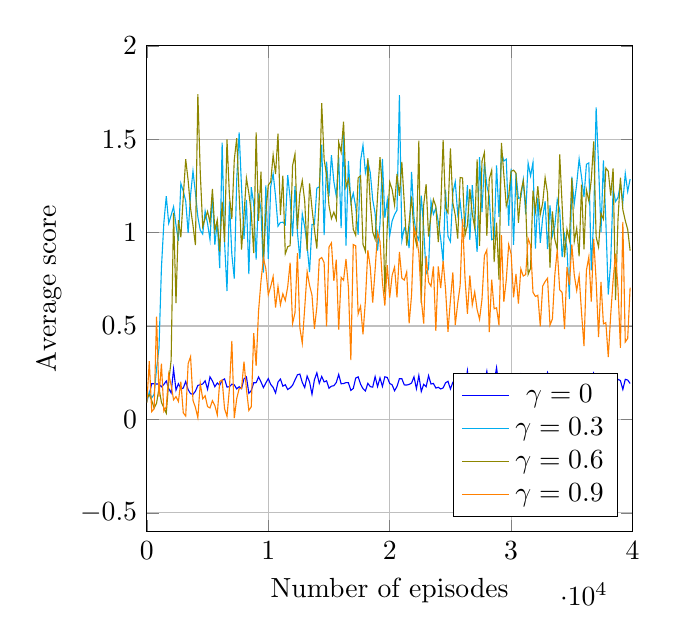
\begin{tikzpicture}
\begin{axis}[height=7.75cm, width=7.75cm, grid=major, xlabel=Number of episodes, ylabel=Average score, xmin=0, xmax=40000, ymin=-0.6, ymax=2, legend pos=south east]
\addplot[blue] coordinates {
(0, 0.1108137) (200, 0.13420482) (400, 0.19165753) (600, 0.19073336) (800, 0.18983261) (1000, 0.18992934) (1200, 0.1746448) (1400, 0.1872443) (1600, 0.20580797) (1800, 0.16505611) (2000, 0.14202482) (2200, 0.26941326) (2400, 0.15724862) (2600, 0.1914621) (2800, 0.16432913) (3000, 0.16796018) (3200, 0.20350736) (3400, 0.15939075) (3600, 0.13783507) (3800, 0.13406035) (4000, 0.15111938) (4200, 0.18197082) (4400, 0.1859607) (4600, 0.18985458) (4800, 0.20703788) (5000, 0.16122256) (5200, 0.22796156) (5400, 0.20591548) (5600, 0.17531975) (5800, 0.19485235) (6000, 0.18244421) (6200, 0.20921065) (6400, 0.21699926) (6600, 0.17323202) (6800, 0.17537647) (7000, 0.1887354) (7200, 0.1853089) (7400, 0.163274) (7600, 0.17511429) (7800, 0.16496809) (8000, 0.21703255) (8200, 0.22756998) (8400, 0.13989511) (8600, 0.15381049) (8800, 0.19628981) (9000, 0.19668703) (9200, 0.22717965) (9400, 0.2008141) (9600, 0.17034635) (9800, 0.19529916) (10000, 0.21864584) (10200, 0.18762022) (10400, 0.17137252) (10600, 0.14179312) (10800, 0.19959697) (11000, 0.21637423) (11200, 0.17804147) (11400, 0.18573011) (11600, 0.16040157) (11800, 0.16908222) (12000, 0.18219848) (12200, 0.21107253) (12400, 0.2386208) (12600, 0.24291055) (12800, 0.1981027) (13000, 0.17024687) (13200, 0.23223379) (13400, 0.20076053) (13600, 0.1349968) (13800, 0.21272646) (14000, 0.24945916) (14200, 0.19316694) (14400, 0.22994606) (14600, 0.20079382) (14800, 0.20699684) (15000, 0.16697015) (15200, 0.17798091) (15400, 0.18054861) (15600, 0.19766709) (15800, 0.24065866) (16000, 0.19094518) (16200, 0.19214286) (16400, 0.19717984) (16600, 0.19642183) (16800, 0.15554737) (17000, 0.16583909) (17200, 0.22135429) (17400, 0.22818062) (17600, 0.18877278) (17800, 0.16492042) (18000, 0.15245861) (18200, 0.19330671) (18400, 0.17570178) (18600, 0.17281137) (18800, 0.2291132) (19000, 0.17592777) (19200, 0.22212443) (19400, 0.17658082) (19600, 0.2282291) (19800, 0.2246772) (20000, 0.1924728) (20200, 0.18513043) (20400, 0.15357031) (20600, 0.17621723) (20800, 0.21804872) (21000, 0.21787736) (21200, 0.1847183) (21400, 0.18409917) (21600, 0.1875859) (21800, 0.19476813) (22000, 0.22808738) (22200, 0.16435175) (22400, 0.2350014) (22600, 0.14979874) (22800, 0.1880164) (23000, 0.1752579) (23200, 0.23438865) (23400, 0.18941909) (23600, 0.1927096) (23800, 0.16787286) (24000, 0.17203452) (24200, 0.16315846) (24400, 0.16875304) (24600, 0.19595447) (24800, 0.20416446) (25000, 0.16286504) (25200, 0.19851741) (25400, 0.19116493) (25600, 0.1753456) (25800, 0.21223372) (26000, 0.20368873) (26200, 0.17705546) (26400, 0.26052925) (26600, 0.14056198) (26800, 0.17759445) (27000, 0.16969696) (27200, 0.17055316) (27400, 0.19698939) (27600, 0.18734168) (27800, 0.1916012) (28000, 0.25817078) (28200, 0.1632284) (28400, 0.15054971) (28600, 0.19917461) (28800, 0.2775105) (29000, 0.17601667) (29200, 0.188286) (29400, 0.23374613) (29600, 0.24041225) (29800, 0.21367459) (30000, 0.19769424) (30200, 0.15009744) (30400, 0.17663696) (30600, 0.19313054) (30800, 0.23738086) (31000, 0.16613844) (31200, 0.1583991) (31400, 0.21719334) (31600, 0.20194548) (31800, 0.17435004) (32000, 0.17236236) (32200, 0.15374233) (32400, 0.17782131) (32600, 0.18494213) (32800, 0.21168864) (33000, 0.25106776) (33200, 0.20021245) (33400, 0.20140779) (33600, 0.16428247) (33800, 0.1778414) (34000, 0.18566398) (34200, 0.19384423) (34400, 0.20717478) (34600, 0.19494139) (34800, 0.19960196) (35000, 0.20695907) (35200, 0.21195877) (35400, 0.21780019) (35600, 0.20157808) (35800, 0.23279016) (36000, 0.16262196) (36200, 0.20610355) (36400, 0.20483398) (36600, 0.12269164) (36800, 0.24730502) (37000, 0.22050586) (37200, 0.19783066) (37400, 0.2237751) (37600, 0.214218) (37800, 0.16131201) (38000, 0.1888054) (38200, 0.17139806) (38400, 0.1495807) (38600, 0.18751763) (38800, 0.21457547) (39000, 0.2079972) (39200, 0.16052546) (39400, 0.21480636) (39600, 0.21077898) (39800, 0.19255595)
};
\addlegendentry{$\gamma = 0$}

\addplot[cyan] coordinates {
(0, 0.09177353) (200, 0.14668062) (400, 0.11537433) (600, 0.13489518) (800, 0.27106217) (1000, 0.38204896) (1200, 0.810668) (1400, 1.0516368) (1600, 1.1949939) (1800, 1.0497788) (2000, 1.0930935) (2200, 1.1385326) (2400, 1.0405561) (2600, 0.95590115) (2800, 1.2627935) (3000, 1.2215972) (3200, 1.1696808) (3400, 0.99817544) (3600, 1.2005342) (3800, 1.3299109) (4000, 1.2129674) (4200, 1.0839549) (4400, 1.0127448) (4600, 0.992237) (4800, 1.1145093) (5000, 1.048187) (5200, 0.9625039) (5400, 1.2009281) (5600, 0.9350903) (5800, 1.0601128) (6000, 0.81036377) (6200, 1.481682) (6400, 0.94772947) (6600, 0.6876121) (6800, 1.1666322) (7000, 0.88243353) (7200, 0.75445575) (7400, 1.2824908) (7600, 1.5358617) (7800, 1.2392899) (8000, 0.9669867) (8200, 1.1749494) (8400, 0.77738154) (8600, 1.2431176) (8800, 1.153192) (9000, 0.8556154) (9200, 1.2094693) (9400, 1.1201724) (9600, 0.7865256) (9800, 1.2522851) (10000, 0.8599448) (10200, 1.2457589) (10400, 1.3157665) (10600, 1.1945039) (10800, 1.0343933) (11000, 1.0544888) (11200, 1.0555148) (11400, 1.0432112) (11600, 1.3081709) (11800, 1.1831977) (12000, 0.9800553) (12200, 1.248428) (12400, 1.0015173) (12600, 0.859072) (12800, 1.1005355) (13000, 1.030961) (13200, 0.92959166) (13400, 0.7886473) (13600, 1.044099) (13800, 1.0431619) (14000, 1.2378228) (14200, 1.2451422) (14400, 1.4708004) (14600, 0.9869186) (14800, 1.3793933) (15000, 1.1939598) (15200, 1.4151837) (15400, 1.2734896) (15600, 1.1957868) (15800, 1.4029306) (16000, 1.0239823) (16200, 1.5374326) (16400, 0.9306878) (16600, 1.3833573) (16800, 1.1617246) (17000, 1.2111071) (17200, 1.1387072) (17400, 0.9883189) (17600, 1.3841432) (17800, 1.4683499) (18000, 1.3212043) (18200, 1.3815472) (18400, 1.3209473) (18600, 1.1763971) (18800, 1.1021771) (19000, 0.9038364) (19200, 1.0461813) (19400, 1.3946766) (19600, 1.079742) (19800, 1.1729118) (20000, 0.984996) (20200, 1.062159) (20400, 1.0968671) (20600, 1.1198198) (20800, 1.7363436) (21000, 0.95781386) (21200, 1.0246763) (21400, 0.999412) (21600, 0.9166928) (21800, 1.3249404) (22000, 1.0803363) (22200, 0.9881318) (22400, 0.9591247) (22600, 1.1983544) (22800, 1.0199813) (23000, 0.7804303) (23200, 0.80599356) (23400, 1.1655166) (23600, 1.0983083) (23800, 1.1315653) (24000, 1.0585846) (24200, 0.9672774) (24400, 0.8442546) (24600, 1.230338) (24800, 0.9804112) (25000, 0.95175004) (25200, 1.2118527) (25400, 1.2719957) (25600, 1.098941) (25800, 1.1653533) (26000, 1.038177) (26200, 1.0315142) (26400, 1.2540438) (26600, 0.96067595) (26800, 1.254556) (27000, 1.0517409) (27200, 0.8967094) (27400, 1.4044014) (27600, 1.109346) (27800, 1.3804089) (28000, 1.2508888) (28200, 1.1926215) (28400, 0.962256) (28600, 0.9679036) (28800, 1.3602759) (29000, 1.0842744) (29200, 1.430969) (29400, 1.3830016) (29600, 1.3930477) (29800, 1.0369003) (30000, 1.3419491) (30200, 0.93387073) (30400, 1.3162979) (30600, 1.1831548) (30800, 1.1884286) (31000, 1.2823824) (31200, 1.0997623) (31400, 1.371907) (31600, 1.3038634) (31800, 1.375283) (32000, 0.9138801) (32200, 1.1862963) (32400, 0.94577646) (32600, 1.0801184) (32800, 1.1677607) (33000, 0.91199857) (33200, 1.1462725) (33400, 0.9841406) (33600, 1.0355414) (33800, 1.1761224) (34000, 1.1215988) (34200, 0.86890787) (34400, 0.98767596) (34600, 0.9159189) (34800, 0.6437498) (35000, 1.2992207) (35200, 1.1545068) (35400, 1.2610155) (35600, 1.3939831) (35800, 1.2970384) (36000, 1.1898886) (36200, 1.3656108) (36400, 1.3732243) (36600, 0.7983232) (36800, 1.0773724) (37000, 1.6701288) (37200, 1.3633071) (37400, 1.0027219) (37600, 1.3871679) (37800, 1.0616069) (38000, 0.6689425) (38200, 0.8431977) (38400, 1.2336488) (38600, 1.1669109) (38800, 1.1873684) (39000, 1.2628053) (39200, 1.1630826) (39400, 1.3163402) (39600, 1.2202379) (39800, 1.286632)
};
\addlegendentry{$\gamma = 0.3$}

\addplot[olive] coordinates {
(0, 0.114373736) (200, 0.13216372) (400, 0.102207236) (600, 0.06023587) (800, 0.08706975) (1000, 0.16802567) (1200, 0.09178192) (1400, 0.06229343) (1600, 0.032954838) (1800, 0.19727562) (2000, 0.31769127) (2200, 1.1060447) (2400, 0.62243253) (2600, 1.0670714) (2800, 0.9750187) (3000, 1.1927947) (3200, 1.3926451) (3400, 1.2793013) (3600, 1.1306211) (3800, 1.0378945) (4000, 0.93375635) (4200, 1.741591) (4400, 1.319234) (4600, 1.0320835) (4800, 1.0761119) (5000, 1.113182) (5200, 1.0537367) (5400, 1.2342573) (5600, 1.0099795) (5800, 1.0679953) (6000, 0.8986536) (6200, 1.1652015) (6400, 0.94899154) (6600, 1.4989575) (6800, 1.199244) (7000, 1.0719347) (7200, 1.3896112) (7400, 1.5055668) (7600, 1.2041692) (7800, 0.909286) (8000, 1.0987284) (8200, 1.2923516) (8400, 1.2114866) (8600, 1.1047488) (8800, 0.8899747) (9000, 1.5363458) (9200, 1.0626404) (9400, 1.3269329) (9600, 0.8407374) (9800, 1.108137) (10000, 1.2545319) (10200, 1.271468) (10400, 1.4159187) (10600, 1.3131393) (10800, 1.5300285) (11000, 1.0938932) (11200, 1.304988) (11400, 0.88605744) (11600, 0.9246042) (11800, 0.93049663) (12000, 1.3581859) (12200, 1.4206499) (12400, 1.0188113) (12600, 1.209981) (12800, 1.278714) (13000, 1.1688939) (13200, 0.9022825) (13400, 1.2635553) (13600, 1.1297077) (13800, 1.0153987) (14000, 0.9144564) (14200, 1.1826811) (14400, 1.693541) (14600, 1.3917817) (14800, 1.3082714) (15000, 1.1446754) (15200, 1.0748723) (15400, 1.1098163) (15600, 1.0703192) (15800, 1.4838545) (16000, 1.4303142) (16200, 1.5943905) (16400, 1.2432305) (16600, 1.2853582) (16800, 1.1760083) (17000, 1.0169718) (17200, 0.9853178) (17400, 1.2928897) (17600, 1.3040794) (17800, 0.93759483) (18000, 0.89983076) (18200, 1.3983225) (18400, 1.1546329) (18600, 1.0040381) (18800, 0.96409816) (19000, 1.1956425) (19200, 1.4036152) (19400, 1.2402409) (19600, 0.6722615) (19800, 1.0365618) (20000, 1.2705263) (20200, 1.2302071) (20400, 1.147775) (20600, 1.3135884) (20800, 1.1969203) (21000, 1.3779294) (21200, 1.1598324) (21400, 0.9305422) (21600, 1.0520302) (21800, 1.1931206) (22000, 0.99754155) (22200, 0.9376374) (22400, 1.4918473) (22600, 0.6225479) (22800, 1.1498003) (23000, 1.2591286) (23200, 0.97934073) (23400, 1.094643) (23600, 1.178074) (23800, 1.1407795) (24000, 0.9489633) (24200, 1.127009) (24400, 1.4956229) (24600, 1.1333653) (24800, 1.1069539) (25000, 1.4503217) (25200, 1.1594894) (25400, 1.0929048) (25600, 0.9676335) (25800, 1.2949904) (26000, 1.2923775) (26200, 0.98501426) (26400, 1.0406872) (26600, 1.2335951) (26800, 1.1009403) (27000, 1.0250598) (27200, 1.3918298) (27400, 0.92863834) (27600, 1.3811221) (27800, 1.4288269) (28000, 0.98227686) (28200, 1.2866862) (28400, 1.3345299) (28600, 0.8428077) (28800, 1.0539136) (29000, 0.7483896) (29200, 1.4807036) (29400, 1.3097382) (29600, 1.144073) (29800, 1.1952627) (30000, 1.3278267) (30200, 1.3343583) (30400, 1.3184668) (30600, 1.0526963) (30800, 1.2136139) (31000, 1.2775457) (31200, 1.1472721) (31400, 0.7766392) (31600, 0.8092509) (31800, 1.2245227) (32000, 1.1149732) (32200, 1.2484648) (32400, 1.096667) (32600, 1.1590118) (32800, 1.294902) (33000, 1.2093903) (33200, 0.81290776) (33400, 1.1136607) (33600, 0.963506) (33800, 0.9104237) (34000, 1.4190371) (34200, 1.1480608) (34400, 0.86790913) (34600, 1.0180297) (34800, 0.96018285) (35000, 1.2918487) (35200, 0.952477) (35400, 1.0236623) (35600, 0.8730341) (35800, 1.2571673) (36000, 0.9109055) (36200, 1.2285903) (36400, 1.1697845) (36600, 1.2818509) (36800, 1.4876833) (37000, 0.97698987) (37200, 0.923414) (37400, 1.1036441) (37600, 1.072282) (37800, 1.3459008) (38000, 1.3288336) (38200, 1.1983476) (38400, 1.3443434) (38600, 0.6392976) (38800, 1.0699189) (39000, 1.2939456) (39200, 1.1225553) (39400, 1.0642658) (39600, 1.0168407) (39800, 0.9029072)
};
\addlegendentry{$\gamma = 0.6$}

\addplot[orange] coordinates {
(0, 0.08844571) (200, 0.3125688) (400, 0.042017907) (600, 0.057211947) (800, 0.5506036) (1000, 0.12175058) (1200, 0.2989336) (1400, 0.043957368) (1600, 0.06771101) (1800, 0.2425527) (2000, 0.18336277) (2200, 0.105170086) (2400, 0.121939786) (2600, 0.096295) (2800, 0.20235196) (3000, 0.03532095) (3200, 0.017896965) (3400, 0.29767343) (3600, 0.3365787) (3800, 0.102417625) (4000, 0.06407072) (4200, 0.009564867) (4400, 0.19321099) (4600, 0.11043922) (4800, 0.12671833) (5000, 0.068583906) (5200, 0.061378524) (5400, 0.10027546) (5600, 0.07427736) (5800, 0.024331708) (6000, 0.20295274) (6200, 0.21151549) (6400, 0.05763553) (6600, 0.016629381) (6800, 0.16588809) (7000, 0.41985688) (7200, 0.006747248) (7400, 0.11127633) (7600, 0.16450168) (7800, 0.16656645) (8000, 0.30924362) (8200, 0.1633261) (8400, 0.04821021) (8600, 0.06795258) (8800, 0.46232793) (9000, 0.2867409) (9200, 0.5809223) (9400, 0.7402112) (9600, 0.86365604) (9800, 0.80632734) (10000, 0.6676235) (10200, 0.71094954) (10400, 0.7651394) (10600, 0.5991817) (10800, 0.71212935) (11000, 0.61408037) (11200, 0.67236686) (11400, 0.6364005) (11600, 0.70998615) (11800, 0.8393636) (12000, 0.51339185) (12200, 0.57096946) (12400, 0.8896602) (12600, 0.4912126) (12800, 0.40807542) (13000, 0.59627444) (13200, 0.79100704) (13400, 0.71757334) (13600, 0.6657863) (13800, 0.48507687) (14000, 0.6013739) (14200, 0.85697514) (14400, 0.8668246) (14600, 0.839199) (14800, 0.49792367) (15000, 0.9220242) (15200, 0.9449616) (15400, 0.7413948) (15600, 0.8549735) (15800, 0.48083475) (16000, 0.7606133) (16200, 0.7452098) (16400, 0.8585073) (16600, 0.7068463) (16800, 0.3178273) (17000, 0.9359018) (17200, 0.929582) (17400, 0.564449) (17600, 0.6058254) (17800, 0.455449) (18000, 0.63704795) (18200, 0.90585464) (18400, 0.8153099) (18600, 0.6248457) (18800, 0.8019732) (19000, 1.0001484) (19200, 0.9515658) (19400, 0.73582923) (19600, 0.60900223) (19800, 0.82638836) (20000, 0.6518959) (20200, 0.7714888) (20400, 0.81541806) (20600, 0.6536793) (20800, 0.8966974) (21000, 0.75640094) (21200, 0.74598086) (21400, 0.789768) (21600, 0.5142111) (21800, 0.6657399) (22000, 1.0277947) (22200, 0.9770117) (22400, 0.89001524) (22600, 0.6437481) (22800, 0.512594) (23000, 0.87554723) (23200, 0.73521143) (23400, 0.71316755) (23600, 0.81880575) (23800, 0.4739923) (24000, 0.81874776) (24200, 0.7025963) (24400, 0.8489467) (24600, 0.6962565) (24800, 0.46896458) (25000, 0.6380306) (25200, 0.7871565) (25400, 0.50552285) (25600, 0.62170947) (25800, 0.7158336) (26000, 1.0741001) (26200, 0.7585135) (26400, 0.5650346) (26600, 0.771245) (26800, 0.61325336) (27000, 0.6823991) (27200, 0.5874781) (27400, 0.5357539) (27600, 0.64326024) (27800, 0.87703025) (28000, 0.9073156) (28200, 0.4671999) (28400, 0.7480128) (28600, 0.5922831) (28800, 0.5976917) (29000, 0.5033445) (29200, 0.9863134) (29400, 0.6292558) (29600, 0.74755603) (29800, 0.9356684) (30000, 0.8851639) (30200, 0.653126) (30400, 0.77870655) (30600, 0.6194855) (30800, 0.8055292) (31000, 0.7675173) (31200, 0.77574855) (31400, 0.9681696) (31600, 0.9319666) (31800, 0.6803167) (32000, 0.65846574) (32200, 0.6646131) (32400, 0.49879378) (32600, 0.7140102) (32800, 0.73822194) (33000, 0.75605315) (33200, 0.5045701) (33400, 0.53815734) (33600, 0.77561986) (33800, 0.90890414) (34000, 0.6938037) (34200, 0.6798718) (34400, 0.4840723) (34600, 0.8164883) (34800, 0.72111374) (35000, 0.9369026) (35200, 0.7732528) (35400, 0.6902144) (35600, 0.7693088) (35800, 0.57027024) (36000, 0.3931591) (36200, 0.7983466) (36400, 0.87022305) (36600, 0.6312579) (36800, 0.967009) (37000, 0.74296176) (37200, 0.44075868) (37400, 0.7357059) (37600, 0.5117786) (37800, 0.5184314) (38000, 0.3341934) (38200, 0.55903995) (38400, 0.7458015) (38600, 0.8868217) (38800, 0.7039326) (39000, 0.38310787) (39200, 1.0578003) (39400, 0.41463763) (39600, 0.43386215) (39800, 0.70526516)
};
\addlegendentry{$\gamma = 0.9$}

\end{axis}
\end{tikzpicture}

&

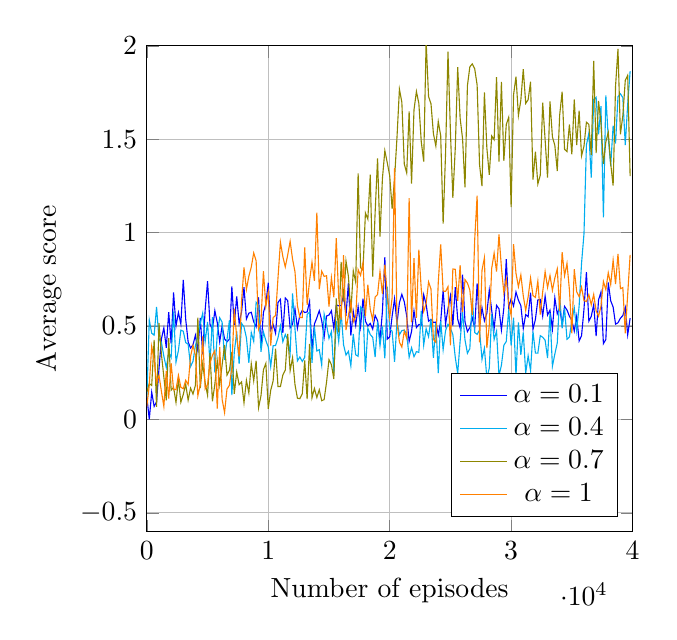
\begin{tikzpicture}
\begin{axis}[height=7.75cm, width=7.75cm, grid=major, xlabel=Number of episodes, ylabel=Average score, xmin=0, xmax=40000, ymin=-0.6, ymax=2, legend pos=south east]
\addplot[blue] coordinates {
(0, 0.12100012) (200, 0.0) (400, 0.14579876) (600, 0.069749445) (800, 0.09473005) (1000, 0.27226627) (1200, 0.4312078) (1400, 0.49019876) (1600, 0.38297018) (1800, 0.5743923) (2000, 0.40572938) (2200, 0.6795475) (2400, 0.5005827) (2600, 0.5726211) (2800, 0.51016706) (3000, 0.747171) (3200, 0.5357579) (3400, 0.41496223) (3600, 0.38203377) (3800, 0.399383) (4000, 0.4505363) (4200, 0.36892503) (4400, 0.5431558) (4600, 0.34800372) (4800, 0.5842685) (5000, 0.7396548) (5200, 0.5087449) (5400, 0.4819249) (5600, 0.58217853) (5800, 0.51802343) (6000, 0.41575593) (6200, 0.5019661) (6400, 0.43078288) (6600, 0.41554275) (6800, 0.42963398) (7000, 0.7114587) (7200, 0.5048429) (7400, 0.6591075) (7600, 0.51362944) (7800, 0.57573885) (8000, 0.7080062) (8200, 0.53771657) (8400, 0.56874335) (8600, 0.5736254) (8800, 0.5219649) (9000, 0.49615183) (9200, 0.65383214) (9400, 0.3900772) (9600, 0.5721787) (9800, 0.61883104) (10000, 0.7314259) (10200, 0.4792521) (10400, 0.507249) (10600, 0.46151254) (10800, 0.626393) (11000, 0.64323205) (11200, 0.4629305) (11400, 0.65009505) (11600, 0.6358013) (11800, 0.4899741) (12000, 0.50963706) (12200, 0.592891) (12400, 0.48839954) (12600, 0.5589961) (12800, 0.5835012) (13000, 0.5724908) (13200, 0.57508737) (13400, 0.6315533) (13600, 0.36960453) (13800, 0.5106714) (14000, 0.5435535) (14200, 0.5821762) (14400, 0.52916116) (14600, 0.44014683) (14800, 0.55381763) (15000, 0.5588697) (15200, 0.5816288) (15400, 0.4856439) (15600, 0.6113994) (15800, 0.60863066) (16000, 0.6094009) (16200, 0.66806877) (16400, 0.55522084) (16600, 0.73111475) (16800, 0.44904542) (17000, 0.5783784) (17200, 0.503352) (17400, 0.60420436) (17600, 0.4951585) (17800, 0.6469207) (18000, 0.52596635) (18200, 0.49985024) (18400, 0.51401764) (18600, 0.4835174) (18800, 0.5566629) (19000, 0.52851987) (19200, 0.42558172) (19400, 0.57684684) (19600, 0.8691173) (19800, 0.42964146) (20000, 0.44204918) (20200, 0.5530558) (20400, 0.64627653) (20600, 0.5135346) (20800, 0.6246005) (21000, 0.669829) (21200, 0.63015) (21400, 0.55356014) (21600, 0.41695952) (21800, 0.4711292) (22000, 0.58213085) (22200, 0.49189347) (22400, 0.50816023) (22600, 0.5053905) (22800, 0.66712093) (23000, 0.61611694) (23200, 0.52588433) (23400, 0.53533655) (23600, 0.5185212) (23800, 0.5212834) (24000, 0.4514329) (24200, 0.5242935) (24400, 0.69067675) (24600, 0.5103582) (24800, 0.59284526) (25000, 0.6620917) (25200, 0.50278085) (25400, 0.7082762) (25600, 0.53663033) (25800, 0.48945463) (26000, 0.7745599) (26200, 0.52304333) (26400, 0.4701645) (26600, 0.49163455) (26800, 0.5435978) (27000, 0.4886727) (27200, 0.72865254) (27400, 0.49567682) (27600, 0.59784454) (27800, 0.52780443) (28000, 0.56811434) (28200, 0.69205767) (28400, 0.5831205) (28600, 0.48615974) (28800, 0.61075765) (29000, 0.59210014) (29200, 0.4791982) (29400, 0.595847) (29600, 0.8574349) (29800, 0.6004485) (30000, 0.6457027) (30200, 0.6072425) (30400, 0.6819289) (30600, 0.6381017) (30800, 0.6096876) (31000, 0.48653933) (31200, 0.5616436) (31400, 0.5493718) (31600, 0.6785934) (31800, 0.48232833) (32000, 0.53585285) (32200, 0.63984054) (32400, 0.64261407) (32600, 0.5534364) (32800, 0.6603948) (33000, 0.5594038) (33200, 0.58488506) (33400, 0.4842522) (33600, 0.6512625) (33800, 0.56503695) (34000, 0.5967865) (34200, 0.5101198) (34400, 0.6052306) (34600, 0.58593667) (34800, 0.5524549) (35000, 0.5306865) (35200, 0.47272426) (35400, 0.5527172) (35600, 0.41992062) (35800, 0.44821876) (36000, 0.59060407) (36200, 0.7877937) (36400, 0.52622217) (36600, 0.5524082) (36800, 0.61392576) (37000, 0.44581294) (37200, 0.6400866) (37400, 0.6816488) (37600, 0.40567982) (37800, 0.42784387) (38000, 0.73338044) (38200, 0.63541526) (38400, 0.60168684) (38600, 0.5100649) (38800, 0.5175132) (39000, 0.5418298) (39200, 0.5559935) (39400, 0.60015076) (39600, 0.45245466) (39800, 0.5422008)
};
\addlegendentry{$\alpha = 0.1$}

\addplot[cyan] coordinates {
(0, 0.11700162) (200, 0.53214467) (400, 0.46151707) (600, 0.45108694) (800, 0.6023132) (1000, 0.42964882) (1200, 0.41226175) (1400, 0.33821237) (1600, 0.27717602) (1800, 0.3577704) (2000, 0.33106858) (2200, 0.5779936) (2400, 0.3068004) (2600, 0.36889082) (2800, 0.47801667) (3000, 0.47206283) (3200, 0.411242) (3400, 0.4028334) (3600, 0.28331468) (3800, 0.31130132) (4000, 0.3951028) (4200, 0.4458365) (4400, 0.51454127) (4600, 0.568677) (4800, 0.41607943) (5000, 0.52189887) (5200, 0.29502952) (5400, 0.5476205) (5600, 0.250214) (5800, 0.4564882) (6000, 0.54418427) (6200, 0.52045405) (6400, 0.31897143) (6600, 0.42698544) (6800, 0.53066415) (7000, 0.12979965) (7200, 0.35858393) (7400, 0.47079378) (7600, 0.29756925) (7800, 0.514491) (8000, 0.49522343) (8200, 0.4372515) (8400, 0.30344155) (8600, 0.46508655) (8800, 0.4180413) (9000, 0.62733656) (9200, 0.6115139) (9400, 0.36171484) (9600, 0.46856043) (9800, 0.42211542) (10000, 0.38688824) (10200, 0.28338403) (10400, 0.3945599) (10600, 0.3956527) (10800, 0.4373426) (11000, 0.50136024) (11200, 0.4155658) (11400, 0.45479017) (11600, 0.425113) (11800, 0.35316613) (12000, 0.6741194) (12200, 0.48428947) (12400, 0.31323254) (12600, 0.3343333) (12800, 0.31036952) (13000, 0.33242574) (13200, 0.56230974) (13400, 0.5745346) (13600, 0.3026983) (13800, 0.49723858) (14000, 0.36631572) (14200, 0.37325993) (14400, 0.29071608) (14600, 0.5638486) (14800, 0.5053047) (15000, 0.43332154) (15200, 0.4703533) (15400, 0.25021422) (15600, 0.52759516) (15800, 0.41767606) (16000, 0.5725401) (16200, 0.39922678) (16400, 0.34465665) (16600, 0.36487237) (16800, 0.28662795) (17000, 0.45741293) (17200, 0.3461027) (17400, 0.3380228) (17600, 0.6025108) (17800, 0.58767444) (18000, 0.254947) (18200, 0.4887133) (18400, 0.45385152) (18600, 0.4398406) (18800, 0.33334464) (19000, 0.52306587) (19200, 0.3932955) (19400, 0.49771848) (19600, 0.3265933) (19800, 0.7104679) (20000, 0.48202637) (20200, 0.4725105) (20400, 0.30827513) (20600, 0.5260518) (20800, 0.45334575) (21000, 0.4755533) (21200, 0.478272) (21400, 0.45877248) (21600, 0.33298245) (21800, 0.38390964) (22000, 0.33593413) (22200, 0.36290708) (22400, 0.3587856) (22600, 0.58154744) (22800, 0.3979755) (23000, 0.4859225) (23200, 0.44318548) (23400, 0.5379004) (23600, 0.32925314) (23800, 0.5148504) (24000, 0.24738318) (24200, 0.52759045) (24400, 0.37337533) (24600, 0.4756759) (24800, 0.5092585) (25000, 0.48916832) (25200, 0.45383245) (25400, 0.33174628) (25600, 0.24641542) (25800, 0.41878706) (26000, 0.5739777) (26200, 0.4259858) (26400, 0.3542561) (26600, 0.379045) (26800, 0.64791715) (27000, 0.4648808) (27200, 0.45567432) (27400, 0.47843918) (27600, 0.3213735) (27800, 0.38098896) (28000, 0.22074789) (28200, 0.27398682) (28400, 0.5633545) (28600, 0.42789596) (28800, 0.4727374) (29000, 0.23425789) (29200, 0.28965566) (29400, 0.39691675) (29600, 0.41746533) (29800, 0.59192514) (30000, 0.39523852) (30200, 0.5445659) (30400, 0.23227383) (30600, 0.51953936) (30800, 0.34600955) (31000, 0.4660334) (31200, 0.2474278) (31400, 0.34076598) (31600, 0.26069173) (31800, 0.47163656) (32000, 0.35487717) (32200, 0.35459846) (32400, 0.44869876) (32600, 0.4399285) (32800, 0.42407006) (33000, 0.3285429) (33200, 0.5695385) (33400, 0.28425342) (33600, 0.34998217) (33800, 0.40956974) (34000, 0.65902865) (34200, 0.48722553) (34400, 0.5967578) (34600, 0.42923552) (34800, 0.4410258) (35000, 0.529662) (35200, 0.5966118) (35400, 0.47525513) (35600, 0.60716474) (35800, 0.8362436) (36000, 0.99379027) (36200, 1.4693363) (36400, 1.5314237) (36600, 1.294107) (36800, 1.7129588) (37000, 1.7247368) (37200, 1.526573) (37400, 1.6769814) (37600, 1.081266) (37800, 1.7346356) (38000, 1.508373) (38200, 1.357931) (38400, 1.5720273) (38600, 1.4773066) (38800, 1.7276202) (39000, 1.7432231) (39200, 1.7225597) (39400, 1.4688513) (39600, 1.6871856) (39800, 1.8644918)
};
\addlegendentry{$\alpha = 0.4$}

\addplot[olive] coordinates {
(0, 0.14671084) (200, 0.19222088) (400, 0.18174548) (600, 0.4253393) (800, 0.06670879) (1000, 0.5156897) (1200, 0.34875724) (1400, 0.22734243) (1600, 0.102233596) (1800, 0.43494686) (2000, 0.15667808) (2200, 0.17188434) (2400, 0.0911331) (2600, 0.2146266) (2800, 0.09210057) (3000, 0.13396998) (3200, 0.18876497) (3400, 0.10308675) (3600, 0.16762023) (3800, 0.13597682) (4000, 0.18267198) (4200, 0.54531765) (4400, 0.16730486) (4600, 0.2992063) (4800, 0.19662108) (5000, 0.12953132) (5200, 0.35527256) (5400, 0.09669439) (5600, 0.18871485) (5800, 0.31463385) (6000, 0.185337) (6200, 0.29169488) (6400, 0.3992299) (6600, 0.23692727) (6800, 0.26247996) (7000, 0.36112472) (7200, 0.13763721) (7400, 0.25375003) (7600, 0.18620275) (7800, 0.20067617) (8000, 0.08891209) (8200, 0.20896529) (8400, 0.14129065) (8600, 0.29851946) (8800, 0.20693335) (9000, 0.3139326) (9200, 0.0630875) (9400, 0.12705885) (9600, 0.2655219) (9800, 0.29994303) (10000, 0.057341143) (10200, 0.15576902) (10400, 0.20625034) (10600, 0.37873942) (10800, 0.1761191) (11000, 0.17593478) (11200, 0.2379451) (11400, 0.26370057) (11600, 0.4579447) (11800, 0.26095405) (12000, 0.33000937) (12200, 0.18635814) (12400, 0.11379452) (12600, 0.111162074) (12800, 0.1372936) (13000, 0.31569678) (13200, 0.109000295) (13400, 0.40399882) (13600, 0.11572214) (13800, 0.16582529) (14000, 0.11747199) (14200, 0.1591559) (14400, 0.100044824) (14600, 0.10626057) (14800, 0.20035324) (15000, 0.32051954) (15200, 0.29311946) (15400, 0.21634021) (15600, 0.64831567) (15800, 0.46561074) (16000, 0.8435192) (16200, 0.6307743) (16400, 0.8482665) (16600, 0.7658029) (16800, 0.5711674) (17000, 0.7959224) (17200, 0.73494345) (17400, 1.3175625) (17600, 0.81228805) (17800, 0.79980433) (18000, 1.1054116) (18200, 1.0722917) (18400, 1.3105057) (18600, 0.76463217) (18800, 1.1077446) (19000, 1.3972456) (19200, 0.978203) (19400, 1.2892029) (19600, 1.439046) (19800, 1.3742573) (20000, 1.3046252) (20200, 1.1278743) (20400, 1.2911427) (20600, 1.5091602) (20800, 1.7677581) (21000, 1.69814) (21200, 1.3674678) (21400, 1.3196108) (21600, 1.649287) (21800, 1.2621584) (22000, 1.6564772) (22200, 1.7555172) (22400, 1.6919547) (22600, 1.4862046) (22800, 1.380577) (23000, 2.0239215) (23200, 1.7278683) (23400, 1.6900953) (23600, 1.529793) (23800, 1.4638022) (24000, 1.5946436) (24200, 1.5185921) (24400, 1.0481112) (24600, 1.42355) (24800, 1.9681895) (25000, 1.5426188) (25200, 1.1862081) (25400, 1.4520158) (25600, 1.8856586) (25800, 1.6128215) (26000, 1.5033374) (26200, 1.2428368) (26400, 1.7865162) (26600, 1.8878517) (26800, 1.9032749) (27000, 1.8773462) (27200, 1.7902875) (27400, 1.3629616) (27600, 1.2488889) (27800, 1.7503495) (28000, 1.4540778) (28200, 1.309643) (28400, 1.5171622) (28600, 1.4969782) (28800, 1.8328451) (29000, 1.3806952) (29200, 1.8064647) (29400, 1.3837799) (29600, 1.5778188) (29800, 1.617619) (30000, 1.1361455) (30200, 1.7373773) (30400, 1.8351731) (30600, 1.6268833) (30800, 1.7093865) (31000, 1.8750134) (31200, 1.6920081) (31400, 1.7110717) (31600, 1.8074831) (31800, 1.2842796) (32000, 1.4332436) (32200, 1.2602569) (32400, 1.3075002) (32600, 1.6961) (32800, 1.4966866) (33000, 1.2939823) (33200, 1.702838) (33400, 1.5126286) (33600, 1.4669124) (33800, 1.3300041) (34000, 1.6308221) (34200, 1.7542286) (34400, 1.4459997) (34600, 1.4336272) (34800, 1.5785285) (35000, 1.4192584) (35200, 1.7124512) (35400, 1.4688531) (35600, 1.6528089) (35800, 1.4104757) (36000, 1.4628489) (36200, 1.5909729) (36400, 1.5792506) (36600, 1.416032) (36800, 1.9192362) (37000, 1.4260246) (37200, 1.7047482) (37400, 1.5842713) (37600, 1.3676512) (37800, 1.4856877) (38000, 1.5363611) (38200, 1.3689896) (38400, 1.2512364) (38600, 1.7850049) (38800, 1.9837524) (39000, 1.5267016) (39200, 1.6259224) (39400, 1.8146214) (39600, 1.842061) (39800, 1.302305)
};
\addlegendentry{$\alpha = 0.7$}

\addplot[orange] coordinates {
(0, 0.06933696) (200, 0.18390138) (400, 0.39115548) (600, 0.31695116) (800, 0.19896056) (1000, 0.23592865) (1200, 0.15018308) (1400, 0.06963388) (1600, 0.26026517) (1800, 0.11112824) (2000, 0.30123296) (2200, 0.15882477) (2400, 0.16031727) (2600, 0.23625219) (2800, 0.17187908) (3000, 0.16436833) (3200, 0.20964362) (3400, 0.18598343) (3600, 0.33725196) (3800, 0.3970297) (4000, 0.344601) (4200, 0.12664463) (4400, 0.18641235) (4600, 0.44380987) (4800, 0.16341889) (5000, 0.18598147) (5200, 0.2998989) (5400, 0.3432163) (5600, 0.36804774) (5800, 0.057440124) (6000, 0.38866565) (6200, 0.10660349) (6400, 0.036694977) (6600, 0.16248098) (6800, 0.18268129) (7000, 0.27790284) (7200, 0.5930389) (7400, 0.43876588) (7600, 0.33666307) (7800, 0.6349341) (8000, 0.8133027) (8200, 0.6959765) (8400, 0.76629084) (8600, 0.815697) (8800, 0.8911451) (9000, 0.8493092) (9200, 0.48400515) (9400, 0.52845913) (9600, 0.7934238) (9800, 0.60542744) (10000, 0.68016374) (10200, 0.39522776) (10400, 0.5454387) (10600, 0.5561828) (10800, 0.757423) (11000, 0.948698) (11200, 0.871718) (11400, 0.81601024) (11600, 0.880549) (11800, 0.9535347) (12000, 0.85777247) (12200, 0.7901049) (12400, 0.60937846) (12600, 0.5460295) (12800, 0.54491025) (13000, 0.9211903) (13200, 0.613431) (13400, 0.7425866) (13600, 0.84198004) (13800, 0.7414693) (14000, 1.1072849) (14200, 0.6971927) (14400, 0.7935584) (14600, 0.7656882) (14800, 0.76932615) (15000, 0.60403425) (15200, 0.75904554) (15400, 0.6536235) (15600, 0.9702484) (15800, 0.6506283) (16000, 0.5334084) (16200, 0.8788189) (16400, 0.47798502) (16600, 0.5566366) (16800, 0.6305258) (17000, 0.52211875) (17200, 0.5501864) (17400, 0.8018621) (17600, 0.7712379) (17800, 0.8392709) (18000, 0.5525128) (18200, 0.7208776) (18400, 0.5886963) (18600, 0.5321946) (18800, 0.6554497) (19000, 0.66865885) (19200, 0.791643) (19400, 0.6719225) (19600, 0.82893294) (19800, 0.66825515) (20000, 0.5445087) (20200, 0.65146124) (20400, 1.3452168) (20600, 0.5200523) (20800, 0.4140003) (21000, 0.3872049) (21200, 0.47366992) (21400, 0.4344099) (21600, 1.1847155) (21800, 0.5201032) (22000, 0.863525) (22200, 0.5435985) (22400, 0.9091722) (22600, 0.6954627) (22800, 0.5778219) (23000, 0.62075895) (23200, 0.73627496) (23400, 0.69841063) (23600, 0.42867365) (23800, 0.41256413) (24000, 0.73326963) (24200, 0.93733215) (24400, 0.6870228) (24600, 0.6854244) (24800, 0.71107584) (25000, 0.39717415) (25200, 0.8052721) (25400, 0.80343777) (25600, 0.6349861) (25800, 0.8257315) (26000, 0.5742738) (26200, 0.74843824) (26400, 0.7300561) (26600, 0.6925502) (26800, 0.5596221) (27000, 0.9627315) (27200, 1.198401) (27400, 0.41241556) (27600, 0.7981323) (27800, 0.8656155) (28000, 0.38176465) (28200, 0.50174236) (28400, 0.8087459) (28600, 0.89032376) (28800, 0.79106313) (29000, 0.99046046) (29200, 0.81229216) (29400, 0.67812467) (29600, 0.7514731) (29800, 0.61965907) (30000, 0.5569424) (30200, 0.93769544) (30400, 0.7818353) (30600, 0.7101348) (30800, 0.7738215) (31000, 0.66110605) (31200, 0.58367693) (31400, 0.65590394) (31600, 0.7568826) (31800, 0.6631708) (32000, 0.65309834) (32200, 0.7406215) (32400, 0.56091684) (32600, 0.68285453) (32800, 0.79130125) (33000, 0.70635855) (33200, 0.77066195) (33400, 0.69093597) (33600, 0.7568148) (33800, 0.80608433) (34000, 0.5809687) (34200, 0.89578146) (34400, 0.76950705) (34600, 0.8352753) (34800, 0.69436663) (35000, 0.46055558) (35200, 0.8037565) (35400, 0.683111) (35600, 0.65691185) (35800, 0.7078331) (36000, 0.6359015) (36200, 0.63133454) (36400, 0.66771674) (36600, 0.61356246) (36800, 0.66939276) (37000, 0.5813861) (37200, 0.55238914) (37400, 0.6059084) (37600, 0.73824424) (37800, 0.69504285) (38000, 0.7853107) (38200, 0.72253954) (38400, 0.85204536) (38600, 0.72508353) (38800, 0.8864557) (39000, 0.69991916) (39200, 0.7058704) (39400, 0.46048504) (39600, 0.6693627) (39800, 0.88133)
};
\addlegendentry{$\alpha = 1$}

\end{axis}
\end{tikzpicture}

\\

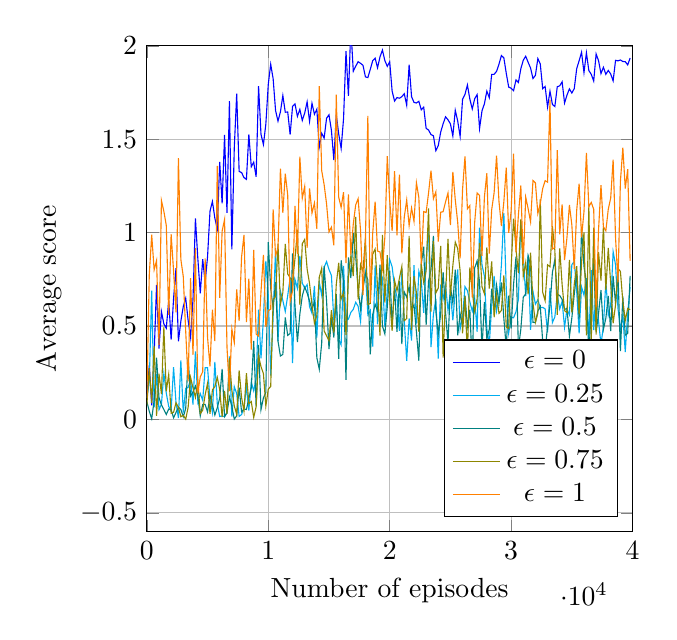
\begin{tikzpicture}
\begin{axis}[height=7.75cm, width=7.75cm, grid=major, xlabel=Number of episodes, ylabel=Average score, xmin=0, xmax=40000, ymin=-0.6, ymax=2, legend pos=south east]
\addplot[blue] coordinates {
(0, 0.11539584) (200, 0.2894594) (400, 0.07506628) (600, 0.34765333) (800, 0.7203276) (1000, 0.37967378) (1200, 0.5771123) (1400, 0.5116135) (1600, 0.48829243) (1800, 0.6362714) (2000, 0.42680895) (2200, 0.64632535) (2400, 0.8095372) (2600, 0.4186643) (2800, 0.52563506) (3000, 0.60470337) (3200, 0.6489253) (3400, 0.5304018) (3600, 0.4402357) (3800, 0.64189696) (4000, 1.0759772) (4200, 0.8595347) (4400, 0.67493945) (4600, 0.858306) (4800, 0.73193175) (5000, 0.87189215) (5200, 1.1143802) (5400, 1.1667696) (5600, 1.0773594) (5800, 1.0197153) (6000, 1.3788666) (6200, 1.1561209) (6400, 1.523445) (6600, 1.1052171) (6800, 1.7040539) (7000, 0.91083604) (7200, 1.4533098) (7400, 1.7438112) (7600, 1.3279284) (7800, 1.3214424) (8000, 1.2947711) (8200, 1.2848771) (8400, 1.5262153) (8600, 1.352658) (8800, 1.377226) (9000, 1.2990739) (9200, 1.7844343) (9400, 1.5265592) (9600, 1.4714985) (9800, 1.5811266) (10000, 1.7942226) (10200, 1.9016706) (10400, 1.8240396) (10600, 1.6534587) (10800, 1.5968543) (11000, 1.6463928) (11200, 1.734005) (11400, 1.6443892) (11600, 1.6459587) (11800, 1.5248417) (12000, 1.6761509) (12200, 1.6887178) (12400, 1.622526) (12600, 1.6595796) (12800, 1.6006029) (13000, 1.6400036) (13200, 1.7001278) (13400, 1.5952499) (13600, 1.6922375) (13800, 1.63404) (14000, 1.6602021) (14200, 1.4582033) (14400, 1.5320226) (14600, 1.5056543) (14800, 1.6121929) (15000, 1.6308615) (15200, 1.5472988) (15400, 1.3885894) (15600, 1.631148) (15800, 1.5278851) (16000, 1.4508686) (16200, 1.6106995) (16400, 1.9717321) (16600, 1.7321709) (16800, 2.0974462) (17000, 1.8639747) (17200, 1.8906277) (17400, 1.9150133) (17600, 1.9063555) (17800, 1.8954667) (18000, 1.8338755) (18200, 1.829792) (18400, 1.8738295) (18600, 1.9201022) (18800, 1.9339273) (19000, 1.8825543) (19200, 1.9405453) (19400, 1.9770131) (19600, 1.9210098) (19800, 1.8900518) (20000, 1.9148475) (20200, 1.7568731) (20400, 1.7043494) (20600, 1.7230583) (20800, 1.7194612) (21000, 1.7278548) (21200, 1.7437079) (21400, 1.6818538) (21600, 1.8989458) (21800, 1.727979) (22000, 1.6970181) (22200, 1.6939766) (22400, 1.702961) (22600, 1.6573961) (22800, 1.6718897) (23000, 1.5578814) (23200, 1.5491896) (23400, 1.5247158) (23600, 1.5182691) (23800, 1.4387176) (24000, 1.4656898) (24200, 1.5384511) (24400, 1.5826684) (24600, 1.6199259) (24800, 1.6039999) (25000, 1.582239) (25200, 1.5171757) (25400, 1.654607) (25600, 1.5974404) (25800, 1.515171) (26000, 1.7140682) (26200, 1.740037) (26400, 1.7903503) (26600, 1.7147769) (26800, 1.6620499) (27000, 1.7169347) (27200, 1.7389104) (27400, 1.5574564) (27600, 1.6512933) (27800, 1.6896957) (28000, 1.7575499) (28200, 1.7224764) (28400, 1.8471891) (28600, 1.8474897) (28800, 1.8633522) (29000, 1.9017955) (29200, 1.9481215) (29400, 1.9356318) (29600, 1.8526658) (29800, 1.7789519) (30000, 1.7732136) (30200, 1.7595972) (30400, 1.8174832) (30600, 1.803681) (30800, 1.8776988) (31000, 1.9227895) (31200, 1.9441184) (31400, 1.9117949) (31600, 1.8813682) (31800, 1.8249545) (32000, 1.8419014) (32200, 1.9316895) (32400, 1.9030696) (32600, 1.7706368) (32800, 1.7822343) (33000, 1.6724733) (33200, 1.7573051) (33400, 1.6860408) (33600, 1.6751482) (33800, 1.7809036) (34000, 1.7857823) (34200, 1.8071644) (34400, 1.6937867) (34600, 1.736337) (34800, 1.7692684) (35000, 1.7473617) (35200, 1.7709515) (35400, 1.877539) (35600, 1.9202278) (35800, 1.965485) (36000, 1.8566499) (36200, 1.9629524) (36400, 1.867437) (36600, 1.8474714) (36800, 1.8114505) (37000, 1.9565315) (37200, 1.9202173) (37400, 1.8513047) (37600, 1.885126) (37800, 1.8472111) (38000, 1.8681632) (38200, 1.8491744) (38400, 1.8121501) (38600, 1.9221333) (38800, 1.9194494) (39000, 1.9240675) (39200, 1.9162097) (39400, 1.9148588) (39600, 1.8978789) (39800, 1.9345655) 
};
\addlegendentry{$\epsilon = 0$}

\addplot[cyan] coordinates {
(0, 0.11243288) (200, 0.20109957) (400, 0.6889083) (600, 0.06459889) (800, 0.24303971) (1000, 0.05282391) (1200, 0.07955645) (1400, 0.2463538) (1600, 0.14100847) (1800, 0.069390215) (2000, 0.04727584) (2200, 0.27973622) (2400, 0.09169855) (2600, 0.007529892) (2800, 0.31580514) (3000, 0.03658371) (3200, 0.16647671) (3400, 0.17059852) (3600, 0.21606088) (3800, 0.07959738) (4000, 0.3643103) (4200, 0.094550274) (4400, 0.13834599) (4600, 0.10200489) (4800, 0.2768246) (5000, 0.27669057) (5200, 0.10822686) (5400, 0.038418267) (5600, 0.3079293) (5800, 0.0836312) (6000, 0.015908724) (6200, 0.018112576) (6400, 0.014717885) (6600, 0.039291613) (6800, 0.33697546) (7000, 0.014946291) (7200, 0.17557253) (7400, 0.13736035) (7600, 0.016595144) (7800, 0.02597868) (8000, 0.06308321) (8200, 0.17508383) (8400, 0.047950175) (8600, 0.19976218) (8800, 0.15285203) (9000, 0.21991712) (9200, 0.5882892) (9400, 0.32675445) (9600, 0.53999954) (9800, 0.8481614) (10000, 0.66392666) (10200, 0.23473947) (10400, 0.5459649) (10600, 0.9172599) (10800, 0.41923058) (11000, 0.68699753) (11200, 0.6361651) (11400, 0.577744) (11600, 0.66255695) (11800, 0.7583939) (12000, 0.30085626) (12200, 0.7488608) (12400, 0.7020476) (12600, 0.8749982) (12800, 0.7290096) (13000, 0.7033056) (13200, 0.721463) (13400, 0.60401285) (13600, 0.5678823) (13800, 0.71424574) (14000, 0.43849617) (14200, 0.7358711) (14400, 0.66409117) (14600, 0.8142603) (14800, 0.84516835) (15000, 0.8026412) (15200, 0.7705994) (15400, 0.5291626) (15600, 0.6134188) (15800, 0.4278769) (16000, 0.39845887) (16200, 0.8216124) (16400, 0.52975255) (16600, 0.5367645) (16800, 0.5729016) (17000, 0.58928293) (17200, 0.6269694) (17400, 0.6054042) (17600, 0.52433723) (17800, 0.7377177) (18000, 0.7913409) (18200, 0.5610877) (18400, 0.5843662) (18600, 0.39035153) (18800, 0.8242777) (19000, 0.50961775) (19200, 0.7936534) (19400, 0.7591157) (19600, 0.49569178) (19800, 0.6913984) (20000, 0.85636467) (20200, 0.81669474) (20400, 0.7081096) (20600, 0.65647227) (20800, 0.4746525) (21000, 0.8085695) (21200, 0.5259146) (21400, 0.3135563) (21600, 0.54099804) (21800, 0.4223365) (22000, 0.8253532) (22200, 0.51365554) (22400, 0.7924709) (22600, 0.7430948) (22800, 0.570663) (23000, 0.85179275) (23200, 1.0284538) (23400, 0.38728225) (23600, 0.56301045) (23800, 0.645632) (24000, 0.32532743) (24200, 0.72205484) (24400, 0.64454424) (24600, 0.7198985) (24800, 0.5837273) (25000, 0.67809117) (25200, 0.5306397) (25400, 0.68716705) (25600, 0.8034976) (25800, 0.48451) (26000, 0.54884636) (26200, 0.71115965) (26400, 0.68945664) (26600, 0.6293193) (26800, 0.57949513) (27000, 0.6465887) (27200, 0.4686299) (27400, 1.0270016) (27600, 0.8278029) (27800, 0.7670388) (28000, 0.4846915) (28200, 0.4011067) (28400, 0.60770017) (28600, 0.7685559) (28800, 0.5819089) (29000, 0.6547178) (29200, 0.82676965) (29400, 1.104705) (29600, 0.69896626) (29800, 0.46313685) (30000, 0.54595315) (30200, 0.5442473) (30400, 0.5767412) (30600, 0.6418735) (30800, 1.0655234) (31000, 0.8755507) (31200, 0.6606937) (31400, 0.8824573) (31600, 0.48015806) (31800, 0.6850641) (32000, 0.6169222) (32200, 0.6407294) (32400, 0.5982561) (32600, 0.59967786) (32800, 0.59193265) (33000, 0.46678492) (33200, 0.7028061) (33400, 0.5183864) (33600, 0.54864717) (33800, 0.6704371) (34000, 0.5910833) (34200, 0.6320567) (34400, 0.4932015) (34600, 0.59022564) (34800, 0.56012565) (35000, 0.82847244) (35200, 0.84593093) (35400, 0.6860696) (35600, 0.4611033) (35800, 0.7088875) (36000, 0.6651227) (36200, 0.7559971) (36400, 0.40903538) (36600, 0.7995563) (36800, 0.47779638) (37000, 0.7171722) (37200, 0.52591056) (37400, 0.401142) (37600, 0.5000894) (37800, 0.73970807) (38000, 0.55823195) (38200, 0.61245924) (38400, 0.8980282) (38600, 0.8276076) (38800, 0.5936813) (39000, 0.48389715) (39200, 0.55526644) (39400, 0.3610663) (39600, 0.56915015) (39800, 0.7102552) 
};
\addlegendentry{$\epsilon = 0.25$}

\addplot[teal] coordinates {
(0, 0.09574668) (200, 0.04337087) (400, 0.0041178227) (600, 0.10006557) (800, 0.33048278) (1000, 0.11612589) (1200, 0.07825337) (1400, 0.053472795) (1600, 0.026508607) (1800, 0.055920966) (2000, 0.052423973) (2200, 0.00877821) (2400, 0.03725811) (2600, 0.06640009) (2800, 0.053159926) (3000, 0.014022467) (3200, 0.05846412) (3400, 0.32938546) (3600, 0.12479679) (3800, 0.14639497) (4000, 0.1783345) (4200, 0.12381618) (4400, 0.01903586) (4600, 0.08034303) (4800, 0.08026111) (5000, 0.039858047) (5200, 0.1283226) (5400, 0.077471055) (5600, 0.023854535) (5800, 0.062304273) (6000, 0.11404129) (6200, 0.270439) (6400, 0.015235468) (6600, 0.035122227) (6800, 0.11978054) (7000, 0.07015026) (7200, 0.0018148705) (7400, 0.019008603) (7600, 0.17124194) (7800, 0.04099006) (8000, 0.055973984) (8200, 0.05331218) (8400, 0.11196725) (8600, 0.16812393) (8800, 0.4199582) (9000, 0.068872444) (9200, 0.3985944) (9400, 0.052229546) (9600, 0.11520269) (9800, 0.14485088) (10000, 0.94867456) (10200, 0.701162) (10400, 0.59733266) (10600, 0.7350301) (10800, 0.41865158) (11000, 0.33938387) (11200, 0.34845558) (11400, 0.54614276) (11600, 0.44995233) (11800, 0.46019357) (12000, 0.8893045) (12200, 0.61045194) (12400, 0.41405204) (12600, 0.5641948) (12800, 0.6608908) (13000, 0.7088897) (13200, 0.67689466) (13400, 0.6340936) (13600, 0.58595926) (13800, 0.63104314) (14000, 0.33010224) (14200, 0.26873693) (14400, 0.40948543) (14600, 0.82119244) (14800, 0.6350513) (15000, 0.37669438) (15200, 0.5418162) (15400, 0.4386648) (15600, 0.67129105) (15800, 0.32459754) (16000, 0.8518958) (16200, 0.7372826) (16400, 0.21128012) (16600, 0.86720145) (16800, 0.75684893) (17000, 0.99725103) (17200, 0.87239045) (17400, 0.69568896) (17600, 0.59018487) (17800, 0.7012181) (18000, 0.7815079) (18200, 0.74772644) (18400, 0.3489764) (18600, 0.56138515) (18800, 0.616) (19000, 0.5804596) (19200, 0.8290332) (19400, 0.4999357) (19600, 0.45768735) (19800, 0.6015107) (20000, 0.7958231) (20200, 0.5042043) (20400, 0.70573705) (20600, 0.4682047) (20800, 0.74048) (21000, 0.40299222) (21200, 0.6823091) (21400, 0.6542281) (21600, 0.7116651) (21800, 0.5879585) (22000, 0.6131734) (22200, 0.46936408) (22400, 0.3142919) (22600, 0.8320821) (22800, 0.92511386) (23000, 0.505792) (23200, 0.7408534) (23400, 0.80070674) (23600, 0.9824492) (23800, 0.5801865) (24000, 0.45759514) (24200, 0.5677966) (24400, 0.78880066) (24600, 0.57124037) (24800, 0.40887657) (25000, 0.7113359) (25200, 0.6226117) (25400, 0.8014426) (25600, 0.44996667) (25800, 0.5653683) (26000, 0.5044778) (26200, 0.6625523) (26400, 0.49861503) (26600, 0.58714163) (26800, 0.28118044) (27000, 0.811443) (27200, 0.8491745) (27400, 0.7330748) (27600, 0.37521848) (27800, 0.62894833) (28000, 0.43056497) (28200, 0.48255545) (28400, 0.7001095) (28600, 0.58174205) (28800, 0.7183423) (29000, 0.62152493) (29200, 0.73357844) (29400, 0.5411625) (29600, 0.3838537) (29800, 0.66261345) (30000, 0.48640454) (30200, 0.72251695) (30400, 0.8708884) (30600, 0.38125834) (30800, 0.48354247) (31000, 0.6543261) (31200, 0.6723398) (31400, 0.8754259) (31600, 0.8250102) (31800, 0.51964355) (32000, 0.5184477) (32200, 0.5804901) (32400, 0.6054297) (32600, 0.41811392) (32800, 0.37185583) (33000, 0.49563953) (33200, 0.60978585) (33400, 0.7870394) (33600, 0.8552502) (33800, 0.66953504) (34000, 0.6634989) (34200, 0.64230376) (34400, 0.58883786) (34600, 0.5943578) (34800, 0.44532365) (35000, 0.543418) (35200, 0.6709332) (35400, 0.7788606) (35600, 0.5342021) (35800, 1.0212408) (36000, 0.8194531) (36200, 0.72886944) (36400, 0.3282607) (36600, 0.61074305) (36800, 0.87588036) (37000, 0.46656808) (37200, 0.5675367) (37400, 0.69257957) (37600, 0.4817117) (37800, 0.5413104) (38000, 0.6616501) (38200, 0.4725603) (38400, 0.7681037) (38600, 0.6189183) (38800, 0.78199375) (39000, 0.36529538) (39200, 0.65835315) (39400, 0.45127672) (39600, 0.46045732) (39800, 0.76798147) 
};
\addlegendentry{$\epsilon = 0.5$}

\addplot[olive] coordinates {
(0, 0.07507303) (200, 0.27451205) (400, 0.08765951) (600, 0.39344656) (800, 0.019766314) (1000, 0.24465077) (1200, 0.13582867) (1400, 0.49378133) (1600, 0.15094319) (1800, 0.24197231) (2000, 0.032618918) (2200, 0.038200006) (2400, 0.0891017) (2600, 0.06417734) (2800, 0.014455342) (3000, 0.021782491) (3200, 0.0014957733) (3400, 0.064912975) (3600, 0.22493225) (3800, 0.16927974) (4000, 0.11777141) (4200, 0.20407277) (4400, 0.031012263) (4600, 0.049434744) (4800, 0.13121112) (5000, 0.19376506) (5200, 0.029595474) (5400, 0.1581978) (5600, 0.17524754) (5800, 0.22565214) (6000, 0.15941134) (6200, 0.012655412) (6400, 0.15319063) (6600, 0.030166766) (6800, 0.32816774) (7000, 0.15532745) (7200, 0.07260036) (7400, 0.026784891) (7600, 0.26223186) (7800, 0.1178291) (8000, 0.04394908) (8200, 0.24763632) (8400, 0.0844868) (8600, 0.09563466) (8800, 0.010689173) (9000, 0.06754226) (9200, 0.3394091) (9400, 0.28317088) (9600, 0.24488355) (9800, 0.071264334) (10000, 0.16193824) (10200, 0.17666315) (10400, 0.641532) (10600, 0.6575791) (10800, 0.9405365) (11000, 0.61596924) (11200, 0.67901206) (11400, 0.9396669) (11600, 0.7786109) (11800, 0.75833577) (12000, 0.7328318) (12200, 0.861426) (12400, 1.0145725) (12600, 0.6127622) (12800, 0.9403453) (13000, 0.963706) (13200, 0.8050865) (13400, 0.72665286) (13600, 0.6130337) (13800, 0.5150198) (14000, 0.55747217) (14200, 0.76102) (14400, 0.8101934) (14600, 0.47383714) (14800, 0.44854432) (15000, 0.42250946) (15200, 0.5854392) (15400, 0.4654156) (15600, 0.7230113) (15800, 0.8384319) (16000, 0.64401346) (16200, 0.6776644) (16400, 0.4527703) (16600, 0.76064855) (16800, 0.8753481) (17000, 0.7672122) (17200, 1.0837413) (17400, 0.64164007) (17600, 0.8293575) (17800, 0.7925014) (18000, 0.9725063) (18200, 0.614295) (18400, 0.6210881) (18600, 0.8846912) (18800, 0.9117528) (19000, 0.71269554) (19200, 0.4491018) (19400, 0.9876629) (19600, 0.6257132) (19800, 0.87989205) (20000, 0.63439894) (20200, 0.47446457) (20400, 0.7445242) (20600, 0.6882918) (20800, 0.7557165) (21000, 0.8190143) (21200, 0.5287388) (21400, 0.5401529) (21600, 0.98281413) (21800, 0.478054) (22000, 0.76631737) (22200, 0.6782814) (22400, 0.4692162) (22600, 0.8311918) (22800, 0.7337283) (23000, 0.79508543) (23200, 1.1295079) (23400, 0.5769224) (23600, 0.95377207) (23800, 0.67752784) (24000, 0.70302606) (24200, 0.9293218) (24400, 0.33131) (24600, 0.6614175) (24800, 0.965878) (25000, 0.66166806) (25200, 0.823668) (25400, 0.9492788) (25600, 0.9147129) (25800, 0.79509306) (26000, 0.4609718) (26200, 0.6587907) (26400, 0.33437315) (26600, 0.8142654) (26800, 0.6830697) (27000, 0.5773029) (27200, 0.6458684) (27400, 0.94434077) (27600, 0.7100688) (27800, 0.6730094) (28000, 0.92100936) (28200, 0.7002854) (28400, 0.8454102) (28600, 0.54719204) (28800, 0.66709423) (29000, 0.56814134) (29200, 0.5835575) (29400, 0.7716057) (29600, 0.49516627) (29800, 0.48591667) (30000, 0.8113728) (30200, 1.0745575) (30400, 0.9124939) (30600, 0.78312325) (30800, 1.0714921) (31000, 0.7656762) (31200, 0.8402727) (31400, 0.66996187) (31600, 0.89251643) (31800, 0.6236904) (32000, 0.5202995) (32200, 0.56824917) (32400, 1.1774075) (32600, 0.6808549) (32800, 0.6356419) (33000, 0.82787204) (33200, 0.81718075) (33400, 1.0342389) (33600, 0.9054728) (33800, 0.5599069) (34000, 0.9160312) (34200, 0.72097856) (34400, 0.5822498) (34600, 0.57199126) (34800, 0.8544759) (35000, 0.5719876) (35200, 0.72480583) (35400, 0.82071894) (35600, 0.5625779) (35800, 0.8401933) (36000, 1.0009246) (36200, 0.44973084) (36400, 1.1453521) (36600, 0.41713324) (36800, 1.0260333) (37000, 0.45469344) (37200, 0.8957078) (37400, 0.7434718) (37600, 1.0339217) (37800, 0.69223833) (38000, 0.9181951) (38200, 0.7267175) (38400, 0.51416206) (38600, 0.61417305) (38800, 0.80776495) (39000, 0.79250306) (39200, 0.631182) (39400, 0.53022885) (39600, 0.5941551) (39800, 0.58722204) 
};
\addlegendentry{$\epsilon = 0.75$}

\addplot[orange] coordinates {
(0, 0.11486556) (200, 0.7738199) (400, 0.98856723) (600, 0.8007949) (800, 0.8508988) (1000, 0.398841) (1200, 1.1720206) (1400, 1.1143688) (1600, 1.0390474) (1800, 0.559873) (2000, 0.9914369) (2200, 0.79550546) (2400, 0.5729537) (2600, 1.3984509) (2800, 0.85690635) (3000, 0.76465696) (3200, 0.4707168) (3400, 0.20347282) (3600, 0.75610846) (3800, 0.34633493) (4000, 0.9175741) (4200, 0.13959835) (4400, 0.22824122) (4600, 0.2549864) (4800, 0.8621014) (5000, 0.43775854) (5200, 0.28403276) (5400, 0.5881322) (5600, 0.4190898) (5800, 1.3574468) (6000, 0.65035826) (6200, 1.0085771) (6400, 1.0703454) (6600, 0.38670534) (6800, 0.15214926) (7000, 0.484456) (7200, 0.41178173) (7400, 0.695448) (7600, 0.5270879) (7800, 0.86921096) (8000, 0.988119) (8200, 0.52061987) (8400, 0.7538775) (8600, 0.37312752) (8800, 0.9079869) (9000, 0.45723063) (9200, 0.44511315) (9400, 0.6838295) (9600, 0.8811824) (9800, 0.49561214) (10000, 0.58186823) (10200, 0.59021986) (10400, 1.1243519) (10600, 0.878577) (10800, 0.91583925) (11000, 1.3420932) (11200, 1.1063914) (11400, 1.3152419) (11600, 1.2017118) (11800, 0.6312587) (12000, 0.6875032) (12200, 1.1431837) (12400, 0.88613135) (12600, 1.4062902) (12800, 1.1840541) (13000, 1.2478962) (13200, 0.91810167) (13400, 1.2366952) (13600, 1.1045166) (13800, 1.1580489) (14000, 1.019914) (14200, 1.7839634) (14400, 1.3315313) (14600, 1.2568471) (14800, 1.1537323) (15000, 1.0038227) (15200, 1.0291961) (15400, 0.9318204) (15600, 1.7379783) (15800, 1.189228) (16000, 1.1353998) (16200, 1.2169412) (16400, 0.8366181) (16600, 1.2047428) (16800, 0.88270575) (17000, 1.0461501) (17200, 1.1485541) (17400, 1.1812986) (17600, 1.0105691) (17800, 0.66553694) (18000, 0.9592632) (18200, 1.6249669) (18400, 0.6250769) (18600, 0.9973744) (18800, 1.1656896) (19000, 0.90116775) (19200, 0.89626193) (19400, 0.8088834) (19600, 0.9747141) (19800, 1.4096208) (20000, 1.172421) (20200, 1.0089833) (20400, 1.3291653) (20600, 0.98494405) (20800, 1.310609) (21000, 0.88901746) (21200, 1.0829812) (21400, 1.1747062) (21600, 1.0376602) (21800, 1.1317807) (22000, 1.0605929) (22200, 1.266504) (22400, 1.187993) (22600, 0.83001244) (22800, 1.1123469) (23000, 1.1076015) (23200, 1.2126436) (23400, 1.3320267) (23600, 1.1816734) (23800, 1.218021) (24000, 0.95245725) (24200, 1.1090243) (24400, 1.1121783) (24600, 1.1647702) (24800, 1.2121757) (25000, 1.0398744) (25200, 1.3253441) (25400, 1.1757109) (25600, 1.0552671) (25800, 0.86275804) (26000, 1.2312833) (26200, 1.4085572) (26400, 1.1275964) (26600, 1.1447835) (26800, 0.65397125) (27000, 1.0563782) (27200, 1.2123709) (27400, 1.199202) (27600, 0.8762512) (27800, 1.19104) (28000, 1.31806) (28200, 0.88740134) (28400, 1.1236709) (28600, 1.2137597) (28800, 1.4124972) (29000, 1.1657212) (29200, 1.0354025) (29400, 1.1649879) (29600, 1.3477048) (29800, 0.99926466) (30000, 1.1141194) (30200, 1.4227185) (30400, 0.89451027) (30600, 1.0951134) (30800, 1.252095) (31000, 0.8327) (31200, 1.1899135) (31400, 1.1283867) (31600, 1.0577188) (31800, 1.2788905) (32000, 1.2662977) (32200, 1.1021271) (32400, 1.1556268) (32600, 1.2361169) (32800, 1.2782125) (33000, 1.2701284) (33200, 1.7105805) (33400, 0.91206384) (33600, 0.9201184) (33800, 1.4419194) (34000, 0.990825) (34200, 1.1508812) (34400, 0.8534983) (34600, 0.97477615) (34800, 1.1480256) (35000, 1.0418583) (35200, 0.804997) (35400, 1.1193936) (35600, 1.2625705) (35800, 0.9750108) (36000, 1.1124755) (36200, 1.4261295) (36400, 1.1389935) (36600, 1.1617306) (36800, 1.1251312) (37000, 0.59952754) (37200, 1.0151112) (37400, 1.2541652) (37600, 1.0311515) (37800, 1.0096116) (38000, 1.1250074) (38200, 1.1852564) (38400, 1.3905498) (38600, 0.9727631) (38800, 0.7337623) (39000, 1.2738237) (39200, 1.4554055) (39400, 1.2362049) (39600, 1.3393171) (39800, 0.8485284)
};
\addlegendentry{$\epsilon = 1$}

\end{axis}
\end{tikzpicture}

&

 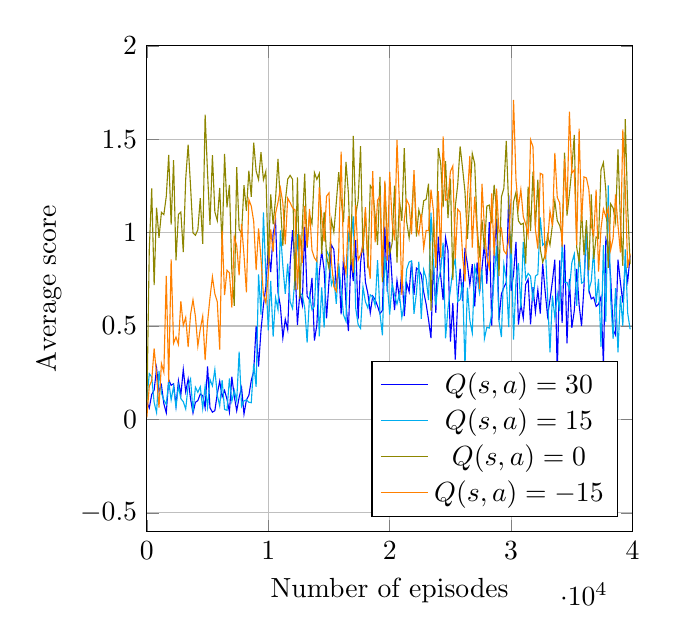
\begin{tikzpicture}
\begin{axis}[height=7.75cm, width=7.75cm, grid=major, xlabel=Number of episodes, ylabel=Average score, xmin=0, xmax=40000, ymin=-0.6, ymax=2, legend pos=south east]
\addplot[blue] coordinates {
(0, 0.09289964) (200, 0.060973193) (400, 0.13339531) (600, 0.15717372) (800, 0.27407843) (1000, 0.15190281) (1200, 0.18364774) (1400, 0.08410699) (1600, 0.035576005) (1800, 0.21259364) (2000, 0.18285246) (2200, 0.19079122) (2400, 0.07531798) (2600, 0.20666483) (2800, 0.13054311) (3000, 0.2676796) (3200, 0.14864) (3400, 0.21513534) (3600, 0.110093325) (3800, 0.034244522) (4000, 0.09155023) (4200, 0.10091768) (4400, 0.13614452) (4600, 0.12730671) (4800, 0.06293483) (5000, 0.2835502) (5200, 0.06218355) (5400, 0.038955472) (5600, 0.046892505) (5800, 0.13762617) (6000, 0.20457767) (6200, 0.120698996) (6400, 0.15530422) (6600, 0.10806368) (6800, 0.039927676) (7000, 0.22845858) (7200, 0.12352985) (7400, 0.046339806) (7600, 0.118058406) (7800, 0.17028566) (8000, 0.028842285) (8200, 0.104624204) (8400, 0.1286508) (8600, 0.2086925) (8800, 0.25894555) (9000, 0.4988489) (9200, 0.2829276) (9400, 0.4770477) (9600, 0.6114826) (9800, 0.7095272) (10000, 0.91900027) (10200, 0.7885581) (10400, 0.9951575) (10600, 1.0614002) (10800, 0.68051547) (11000, 0.60464525) (11200, 0.4364814) (11400, 0.53607297) (11600, 0.48038173) (11800, 0.8327179) (12000, 1.0136075) (12200, 0.82320005) (12400, 0.5051418) (12600, 0.68072414) (12800, 0.61405957) (13000, 1.0303214) (13200, 0.6594455) (13400, 0.6407149) (13600, 0.75712246) (13800, 0.42200938) (14000, 0.50607985) (14200, 0.78337467) (14400, 0.90030444) (14600, 0.80075544) (14800, 0.5408905) (15000, 0.73947936) (15200, 0.9331223) (15400, 0.90963924) (15600, 0.7066508) (15800, 0.81505406) (16000, 0.5622283) (16200, 0.8816163) (16400, 0.6178194) (16600, 0.47253716) (16800, 0.8585453) (17000, 0.7405716) (17200, 0.9591957) (17400, 0.5363403) (17600, 0.83721685) (17800, 0.95001376) (18000, 0.7353121) (18200, 0.6744836) (18400, 0.57023734) (18600, 0.66061) (18800, 0.6413551) (19000, 0.60681516) (19200, 0.56588286) (19400, 0.583768) (19600, 1.0314826) (19800, 0.6836933) (20000, 0.9508283) (20200, 0.740909) (20400, 0.5851566) (20600, 0.7438383) (20800, 0.6492697) (21000, 0.79876024) (21200, 0.55340284) (21400, 0.72912204) (21600, 0.68312764) (21800, 0.846987) (22000, 0.66686594) (22200, 0.8101544) (22400, 0.7997542) (22600, 0.7733607) (22800, 0.68289727) (23000, 0.6178163) (23200, 0.5330863) (23400, 0.4349716) (23600, 0.849079) (23800, 0.57022864) (24000, 0.978534) (24200, 0.76903945) (24400, 0.639039) (24600, 0.9733009) (24800, 0.9044333) (25000, 0.41674322) (25200, 0.6231116) (25400, 0.32025257) (25600, 0.6389489) (25800, 0.807448) (26000, 0.6337156) (26200, 0.9176902) (26400, 0.82978106) (26600, 0.72070676) (26800, 0.8307639) (27000, 0.60485023) (27200, 0.84086746) (27400, 0.6813829) (27600, 0.8096781) (27800, 0.9415786) (28000, 0.7264451) (28200, 1.0557346) (28400, 0.501759) (28600, 0.89111215) (28800, 1.0740594) (29000, 0.53332895) (29200, 0.67153037) (29400, 0.70592654) (29600, 0.7334377) (29800, 1.1999453) (30000, 0.68880135) (30200, 0.7770963) (30400, 0.950722) (30600, 0.5075893) (30800, 0.61772627) (31000, 0.54260725) (31200, 0.72298825) (31400, 0.74950457) (31600, 0.509019) (31800, 0.7084784) (32000, 0.574862) (32200, 0.6939472) (32400, 0.5667615) (32600, 0.83408946) (32800, 0.68601197) (33000, 0.5544637) (33200, 0.6402771) (33400, 0.73966753) (33600, 0.85518336) (33800, 0.23661599) (34000, 0.8515456) (34200, 0.5164431) (34400, 0.93620676) (34600, 0.40740108) (34800, 0.752915) (35000, 0.49033356) (35200, 0.5809087) (35400, 0.80524236) (35600, 0.6126301) (35800, 0.50002474) (36000, 0.7127345) (36200, 1.0354931) (36400, 0.69260895) (36600, 0.64532363) (36800, 0.6540899) (37000, 0.6051358) (37200, 0.61671436) (37400, 0.65574014) (37600, 0.2865559) (37800, 0.9657526) (38000, 0.91964155) (38200, 0.7556457) (38400, 0.48080474) (38600, 0.45160908) (38800, 0.8550716) (39000, 0.734764) (39200, 0.6256111) (39400, 0.83199817) (39600, 0.7387443) (39800, 0.8787812) 
};
\addlegendentry{$Q(s, a) = 30$}

\addplot[cyan] coordinates {
(0, 0.10444397) (200, 0.24500218) (400, 0.22738811) (600, 0.090928175) (800, 0.037043363) (1000, 0.2598516) (1200, 0.14111432) (1400, 0.104130186) (1600, 0.08073901) (1800, 0.2027459) (2000, 0.10501476) (2200, 0.17587122) (2400, 0.06495514) (2600, 0.18109816) (2800, 0.11117473) (3000, 0.094878085) (3200, 0.055547338) (3400, 0.18093559) (3600, 0.21691456) (3800, 0.04039671) (4000, 0.17217906) (4200, 0.14539757) (4400, 0.17497163) (4600, 0.058275267) (4800, 0.1795651) (5000, 0.06573324) (5200, 0.21409144) (5400, 0.17983688) (5600, 0.26726064) (5800, 0.12947777) (6000, 0.07246811) (6200, 0.21034436) (6400, 0.05318481) (6600, 0.048839767) (6800, 0.21950397) (7000, 0.09736716) (7200, 0.15520576) (7400, 0.09972902) (7600, 0.3623753) (7800, 0.07022776) (8000, 0.09949358) (8200, 0.10480141) (8400, 0.0921494) (8600, 0.089643836) (8800, 0.29840583) (9000, 0.17455715) (9200, 0.77690166) (9400, 0.56066185) (9600, 1.1077687) (9800, 0.77074033) (10000, 0.47735253) (10200, 0.74179566) (10400, 0.4427824) (10600, 0.6514716) (10800, 0.58762574) (11000, 1.0123436) (11200, 0.8215872) (11400, 0.6716994) (11600, 0.8342133) (11800, 0.63046944) (12000, 0.5935881) (12200, 0.7624563) (12400, 0.9911517) (12600, 0.67908216) (12800, 0.6652447) (13000, 0.59809923) (13200, 0.41173077) (13400, 0.6629467) (13600, 0.58734715) (13800, 0.606319) (14000, 0.87113833) (14200, 0.44421598) (14400, 0.7061953) (14600, 0.4916733) (14800, 0.9054583) (15000, 0.8735115) (15200, 0.7199208) (15400, 0.76038384) (15600, 0.61881816) (15800, 0.8353252) (16000, 0.69143724) (16200, 0.55896896) (16400, 0.5250045) (16600, 0.99449116) (16800, 0.9380553) (17000, 1.0874145) (17200, 0.5955923) (17400, 0.50805575) (17600, 0.48717064) (17800, 0.70964247) (18000, 0.6299671) (18200, 0.59702533) (18400, 0.66710395) (18600, 0.6561253) (18800, 0.6103998) (19000, 0.85224783) (19200, 0.56492484) (19400, 0.4504603) (19600, 0.87186885) (19800, 0.7236674) (20000, 0.56146944) (20200, 0.72625595) (20400, 0.6670217) (20600, 0.6171325) (20800, 0.67197275) (21000, 0.5454474) (21200, 0.6225816) (21400, 0.8040313) (21600, 0.8429786) (21800, 0.8486488) (22000, 0.56497854) (22200, 0.67732435) (22400, 0.84496266) (22600, 0.53830814) (22800, 0.8011149) (23000, 0.7545723) (23200, 0.6390868) (23400, 1.1066163) (23600, 0.835021) (23800, 0.6101321) (24000, 0.7427272) (24200, 0.80110097) (24400, 0.9465195) (24600, 0.43368733) (24800, 0.5946011) (25000, 0.6928855) (25200, 0.80397016) (25400, 0.8567198) (25600, 0.63147295) (25800, 0.6417094) (26000, 0.73413116) (26200, 0.28241527) (26400, 0.70600104) (26600, 0.53086835) (26800, 0.46265528) (27000, 0.81818974) (27200, 0.76296073) (27400, 0.6788455) (27600, 0.8022579) (27800, 0.43210503) (28000, 0.493529) (28200, 0.48919338) (28400, 0.56436515) (28600, 0.76040053) (28800, 0.9272985) (29000, 0.5254161) (29200, 0.440511) (29400, 0.82971174) (29600, 0.7541162) (29800, 0.49388325) (30000, 0.9923416) (30200, 0.42719448) (30400, 0.74692523) (30600, 0.8362805) (30800, 0.59554726) (31000, 0.95015377) (31200, 0.7521028) (31400, 0.78184783) (31600, 0.7662049) (31800, 0.63257813) (32000, 0.76700705) (32200, 0.77687323) (32400, 1.0814766) (32600, 0.9330567) (32800, 0.94763523) (33000, 0.6637571) (33200, 0.35844204) (33400, 0.6628084) (33600, 0.54512006) (33800, 0.6719988) (34000, 0.5802364) (34200, 0.94453686) (34400, 0.73328924) (34600, 0.73369044) (34800, 0.6959413) (35000, 0.8383685) (35200, 0.88515186) (35400, 0.6080162) (35600, 0.8998449) (35800, 0.7293548) (36000, 0.7373104) (36200, 1.0303301) (36400, 0.69255775) (36600, 0.73913616) (36800, 0.91166234) (37000, 0.6228399) (37200, 0.75162) (37400, 0.38917217) (37600, 0.933385) (37800, 0.5229135) (38000, 1.2533059) (38200, 0.64301074) (38400, 0.43120494) (38600, 0.7022138) (38800, 0.35948828) (39000, 0.66159606) (39200, 0.50161713) (39400, 0.91074276) (39600, 0.56874543) (39800, 0.4824447) 
};
\addlegendentry{$Q(s, a) = 15$}

\addplot[olive] coordinates {
(0, 0.057795405) (200, 0.9081013) (400, 1.2366331) (600, 0.7191439) (800, 1.1330097) (1000, 0.9719158) (1200, 1.1085292) (1400, 1.0964438) (1600, 1.193546) (1800, 1.416665) (2000, 1.0422968) (2200, 1.3881131) (2400, 0.8517937) (2600, 1.0978218) (2800, 1.1104236) (3000, 0.8954162) (3200, 1.287753) (3400, 1.4714333) (3600, 1.2471249) (3800, 0.9984255) (4000, 0.98584837) (4200, 1.0153481) (4400, 1.1843265) (4600, 0.9402386) (4800, 1.6320541) (5000, 1.315573) (5200, 1.0418288) (5400, 1.4149021) (5600, 1.1110183) (5800, 1.0642222) (6000, 1.2387036) (6200, 0.92413265) (6400, 1.4213195) (6600, 1.1354117) (6800, 1.255563) (7000, 0.7937868) (7200, 0.6078712) (7400, 1.3507692) (7600, 1.018177) (7800, 0.99536026) (8000, 1.2540325) (8200, 1.1163938) (8400, 1.3311344) (8600, 1.1916226) (8800, 1.482107) (9000, 1.3299845) (9200, 1.2837062) (9400, 1.43011) (9600, 1.2827288) (9800, 1.3280362) (10000, 0.8331783) (10200, 1.2050892) (10400, 1.0437456) (10600, 1.1826239) (10800, 1.3942758) (11000, 1.157856) (11200, 0.928705) (11400, 1.1661549) (11600, 1.2859735) (11800, 1.3064502) (12000, 1.2853434) (12200, 0.69236356) (12400, 1.2957126) (12600, 0.64506185) (12800, 1.034379) (13000, 1.3151883) (13200, 0.91895294) (13400, 1.0944403) (13600, 1.0475756) (13800, 1.3211373) (14000, 1.2851932) (14200, 1.3156711) (14400, 0.88596) (14600, 1.1113198) (14800, 0.87476885) (15000, 0.808131) (15200, 1.0677568) (15400, 1.0027235) (15600, 1.1595962) (15800, 1.3238037) (16000, 1.1776304) (16200, 1.0567656) (16400, 1.3786008) (16600, 1.2100356) (16800, 0.8251591) (17000, 1.5181047) (17200, 1.0944597) (17400, 1.1731285) (17600, 1.4626806) (17800, 0.8929404) (18000, 1.1157863) (18200, 0.8089107) (18400, 1.2520686) (18600, 1.2303593) (18800, 1.0894032) (19000, 0.9339066) (19200, 1.2979631) (19400, 0.7356062) (19600, 1.2679243) (19800, 0.9811024) (20000, 0.8868479) (20200, 0.9434192) (20400, 1.2511961) (20600, 0.8397828) (20800, 1.1754647) (21000, 1.0629355) (21200, 1.4528517) (21400, 1.0577102) (21600, 0.9715985) (21800, 1.0902048) (22000, 1.311136) (22200, 0.9793044) (22400, 1.1213436) (22600, 1.0680513) (22800, 1.1701264) (23000, 1.178137) (23200, 1.262474) (23400, 0.5829813) (23600, 1.0707505) (23800, 0.8101148) (24000, 1.45216) (24200, 1.3706725) (24400, 1.1367253) (24600, 1.383154) (24800, 1.0776521) (25000, 1.289468) (25200, 0.74602056) (25400, 1.1389022) (25600, 1.2558144) (25800, 1.4617643) (26000, 1.3454115) (26200, 1.2187872) (26400, 0.9667389) (26600, 1.1911602) (26800, 1.4236428) (27000, 1.3691114) (27200, 1.0348165) (27400, 0.8665394) (27600, 1.0698156) (27800, 0.9090916) (28000, 1.1420182) (28200, 1.1474388) (28400, 1.0493938) (28600, 1.2559861) (28800, 1.1281532) (29000, 0.76660854) (29200, 1.1913321) (29400, 1.2368728) (29600, 1.4904238) (29800, 1.1377088) (30000, 0.8838388) (30200, 1.1646314) (30400, 1.2162446) (30600, 1.0635244) (30800, 1.0434787) (31000, 1.0500835) (31200, 0.8340387) (31400, 1.2463665) (31600, 1.0087978) (31800, 1.3265238) (32000, 1.0268757) (32200, 1.2840325) (32400, 0.91189384) (32600, 0.84190464) (32800, 0.879703) (33000, 0.9862368) (33200, 0.9334043) (33400, 1.041491) (33600, 1.170272) (33800, 1.0643902) (34000, 1.0380429) (34200, 0.9852803) (34400, 1.428504) (34600, 1.0909284) (34800, 1.2076197) (35000, 1.3425227) (35200, 1.522548) (35400, 0.9221998) (35600, 0.83978647) (35800, 1.1265186) (36000, 0.87971586) (36200, 1.0661192) (36400, 0.7974464) (36600, 1.2049192) (36800, 0.8589108) (37000, 0.9765408) (37200, 0.96892446) (37400, 1.3356423) (37600, 1.3748199) (37800, 1.2245101) (38000, 0.810734) (38200, 1.1536217) (38400, 1.131852) (38600, 1.0557677) (38800, 1.4458098) (39000, 1.0530908) (39200, 0.82175386) (39400, 1.607303) (39600, 1.1284096) (39800, 0.8314484) 
};
\addlegendentry{$Q(s, a) = 0$}

\addplot[orange] coordinates {
(0, 0.010190566) (200, 0.17781399) (400, 0.20688175) (600, 0.38015783) (800, 0.2383676) (1000, 0.06375262) (1200, 0.29910728) (1400, 0.25217327) (1600, 0.7687368) (1800, 0.20090565) (2000, 0.8569621) (2200, 0.40722758) (2400, 0.441121) (2600, 0.40149027) (2800, 0.63275594) (3000, 0.50307375) (3200, 0.54613674) (3400, 0.38777873) (3600, 0.56270355) (3800, 0.640192) (4000, 0.55120087) (4200, 0.39277866) (4400, 0.48448294) (4600, 0.5526371) (4800, 0.3173067) (5000, 0.5224185) (5200, 0.6522506) (5400, 0.76373184) (5600, 0.6725376) (5800, 0.630124) (6000, 0.3735569) (6200, 1.0105551) (6400, 0.6657079) (6600, 0.79879326) (6800, 0.7843026) (7000, 0.5989976) (7200, 0.978241) (7400, 0.9303041) (7600, 0.7711965) (7800, 1.0462608) (8000, 0.8797969) (8200, 0.6798777) (8400, 1.1772262) (8600, 1.1418654) (8800, 1.0595449) (9000, 0.7995103) (9200, 1.0222005) (9400, 0.85924387) (9600, 0.66811883) (9800, 0.6241255) (10000, 0.7750225) (10200, 1.0176986) (10400, 0.89670616) (10600, 1.1023128) (10800, 1.1622434) (11000, 1.2383497) (11200, 1.1586419) (11400, 0.9370659) (11600, 1.184473) (11800, 1.1600586) (12000, 1.1331514) (12200, 1.1212672) (12400, 0.69515926) (12600, 0.99083054) (12800, 0.83629006) (13000, 1.1425328) (13200, 0.93091434) (13400, 1.1265796) (13600, 0.9050788) (13800, 0.8646087) (14000, 0.846164) (14200, 1.2425382) (14400, 1.0886097) (14600, 0.951857) (14800, 1.1950234) (15000, 1.2125627) (15200, 0.8452657) (15400, 0.71052134) (15600, 0.686195) (15800, 0.892748) (16000, 1.4336412) (16200, 0.850799) (16400, 0.7818035) (16600, 1.0880532) (16800, 0.94891155) (17000, 0.78596365) (17200, 1.1467967) (17400, 0.85293263) (17600, 0.8822017) (17800, 0.93568844) (18000, 1.1369418) (18200, 0.85254836) (18400, 0.7533865) (18600, 1.3289865) (18800, 0.9484797) (19000, 1.1741428) (19200, 1.1933868) (19400, 0.76112455) (19600, 1.2787952) (19800, 0.85021025) (20000, 1.3245649) (20200, 1.0568591) (20400, 0.95929086) (20600, 1.4963174) (20800, 1.1559709) (21000, 0.66620314) (21200, 1.067808) (21400, 1.1753757) (21600, 1.1471156) (21800, 0.99084026) (22000, 1.334068) (22200, 1.0325962) (22400, 0.991278) (22600, 1.1005815) (22800, 0.91595244) (23000, 1.0117617) (23200, 1.0103279) (23400, 1.2304608) (23600, 1.1161203) (23800, 0.82178277) (24000, 1.2221403) (24200, 0.8664454) (24400, 1.5151653) (24600, 1.1734871) (24800, 1.1795543) (25000, 1.3268052) (25200, 1.3567649) (25400, 0.86135924) (25600, 1.1251028) (25800, 1.1097442) (26000, 0.8781254) (26200, 0.73889935) (26400, 1.188475) (26600, 1.4109865) (26800, 0.9198374) (27000, 1.1925406) (27200, 1.0041516) (27400, 0.69783837) (27600, 1.2614675) (27800, 1.0273767) (28000, 0.86720926) (28200, 0.80993086) (28400, 1.2095083) (28600, 0.87571985) (28800, 1.2357489) (29000, 1.0040348) (29200, 1.0224192) (29400, 0.9037018) (29600, 0.8855585) (29800, 0.9597948) (30000, 1.1869923) (30200, 1.7106248) (30400, 1.2816608) (30600, 1.1341305) (30800, 1.2307122) (31000, 1.0861189) (31200, 1.0447435) (31400, 0.98358554) (31600, 1.4970764) (31800, 1.4589849) (32000, 1.0172329) (32200, 0.91438866) (32400, 1.3175347) (32600, 1.3106337) (32800, 0.8569397) (33000, 0.94778246) (33200, 1.1163754) (33400, 1.0363144) (33600, 1.4264225) (33800, 1.1883643) (34000, 1.159034) (34200, 0.9221378) (34400, 1.3943127) (34600, 1.1204256) (34800, 1.6480442) (35000, 1.3180782) (35200, 1.3356417) (35400, 0.9330708) (35600, 1.5569907) (35800, 1.0592037) (36000, 1.2983085) (36200, 1.2927277) (36400, 1.2321656) (36600, 1.0378557) (36800, 0.98291034) (37000, 1.2299826) (37200, 0.7909509) (37400, 1.0202732) (37600, 1.1264414) (37800, 1.0847175) (38000, 1.1307443) (38200, 0.9081732) (38400, 0.9707118) (38600, 1.2044872) (38800, 1.0392231) (39000, 0.89273465) (39200, 1.5532025) (39400, 1.2397981) (39600, 0.8116283) (39800, 0.8882611) 
};
\addlegendentry{$Q(s, a) = -15$}

\end{axis}
\end{tikzpicture}

\end{tabular}

\caption{Performance of the independent Q-Learning algorithm for different combinations of its parameters. The ``1 predator versus 1 prey'' scenario was tested. Unless otherwise stated, the parameters used were: $\alpha = 0.9, \gamma = 0.9, \epsilon = 0.1, Q(s, a) = 15$.}
\label{fig:ql-params}
\end{figure}

\newpage

\begin{figure}[ht!]
 \centering
 
 \begin{tabular}{cc}

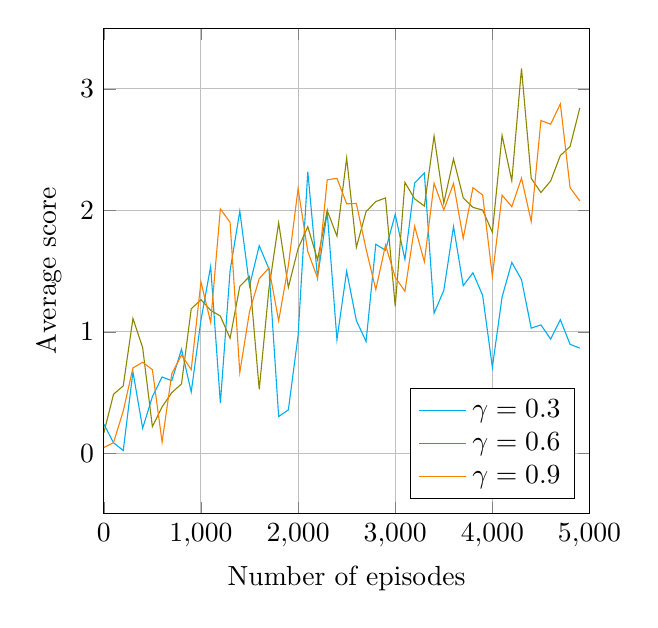
\begin{tikzpicture}
\begin{axis}[height=7.75cm, width=7.75cm, grid=major, xlabel=Number of episodes, ylabel=Average score, xmin=0, xmax=5000, ymin=-0.5, ymax=3.5, legend pos=south east]
% \addplot[blue] coordinates {
% };
% \addlegendentry{$\gamma = 0$}

\addplot[cyan] coordinates {
(0, 0.24019068) (100, 0.086535975) (200, 0.021884544) (300, 0.6695074) (400, 0.20556265) (500, 0.46540916) (600, 0.6276946) (700, 0.5977449) (800, 0.8557811) (900, 0.504657) (1000, 1.0947102) (1100, 1.5386682) (1200, 0.41207418) (1300, 1.5033295) (1400, 1.9939443) (1500, 1.3769149) (1600, 1.7092875) (1700, 1.5175939) (1800, 0.3021351) (1900, 0.3570217) (2000, 0.9693309) (2100, 2.3176484) (2200, 1.4480205) (2300, 1.9855485) (2400, 0.9363186) (2500, 1.4990823) (2600, 1.0925311) (2700, 0.91996855) (2800, 1.7204973) (2900, 1.6718495) (3000, 1.9668694) (3100, 1.5954415) (3200, 2.2254913) (3300, 2.3075585) (3400, 1.1530557) (3500, 1.3405211) (3600, 1.866747) (3700, 1.379714) (3800, 1.4860759) (3900, 1.2998141) (4000, 0.7074839) (4100, 1.2861505) (4200, 1.5714715) (4300, 1.4292024) (4400, 1.0303098) (4500, 1.0564508) (4600, 0.93953514) (4700, 1.099314) (4800, 0.89675003) (4900, 0.86541384)
};
\addlegendentry{$\gamma = 0.3$}

\addplot[olive] coordinates {
(0, 0.16610637) (100, 0.48563656) (200, 0.5540212) (300, 1.1089855) (400, 0.86939836) (500, 0.21821758) (600, 0.38123426) (700, 0.4987786) (800, 0.5707362) (900, 1.1891972) (1000, 1.2644156) (1100, 1.1770762) (1200, 1.1291239) (1300, 0.9470017) (1400, 1.3742715) (1500, 1.4558307) (1600, 0.52523583) (1700, 1.3547359) (1800, 1.8974947) (1900, 1.3656644) (2000, 1.6856433) (2100, 1.8653886) (2200, 1.5939571) (2300, 1.997956) (2400, 1.7877682) (2500, 2.4303896) (2600, 1.6956869) (2700, 1.9895085) (2800, 2.0728118) (2900, 2.1021101) (3000, 1.2098619) (3100, 2.2305248) (3200, 2.0944762) (3300, 2.035708) (3400, 2.6126614) (3500, 2.060516) (3600, 2.4235563) (3700, 2.1030645) (3800, 2.0244393) (3900, 2.0026414) (4000, 1.8198824) (4100, 2.6172874) (4200, 2.2438881) (4300, 3.1694236) (4400, 2.2643862) (4500, 2.1468163) (4600, 2.2421365) (4700, 2.45173) (4800, 2.525833) (4900, 2.84297)
};
\addlegendentry{$\gamma = 0.6$}

\addplot[orange] coordinates {
(0, 0.046459362) (100, 0.086777486) (200, 0.34701955) (300, 0.7021876) (400, 0.74912524) (500, 0.6881235) (600, 0.09215304) (700, 0.65425897) (800, 0.80900145) (900, 0.68840134) (1000, 1.4111269) (1100, 1.0782071) (1200, 2.011735) (1300, 1.901412) (1400, 0.6643786) (1500, 1.1655734) (1600, 1.4373999) (1700, 1.5262848) (1800, 1.0903087) (1900, 1.5450555) (2000, 2.1790001) (2100, 1.6609112) (2200, 1.4441974) (2300, 2.2514858) (2400, 2.2640066) (2500, 2.054192) (2600, 2.05643) (2700, 1.6811329) (2800, 1.3473744) (2900, 1.7148299) (3000, 1.4489069) (3100, 1.333591) (3200, 1.868292) (3300, 1.5771114) (3400, 2.223491) (3500, 2.003037) (3600, 2.2220948) (3700, 1.7694572) (3800, 2.1869361) (3900, 2.1263793) (4000, 1.4574677) (4100, 2.12546) (4200, 2.0298264) (4300, 2.2655075) (4400, 1.9079212) (4500, 2.7400007) (4600, 2.7095385) (4700, 2.8769479) (4800, 2.1872087) (4900, 2.0776663)
};
\addlegendentry{$\gamma = 0.9$}

\end{axis}
\end{tikzpicture}

&

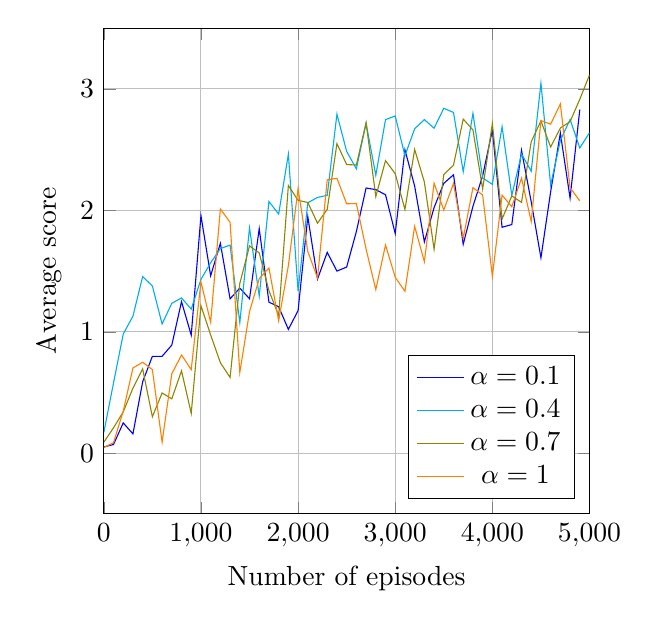
\begin{tikzpicture}
\begin{axis}[height=7.75cm, width=7.75cm, grid=major, xlabel=Number of episodes, ylabel=Average score, xmin=0, xmax=5000, ymin=-0.5, ymax=3.5, legend pos=south east]
\addplot[blue] coordinates {
(0, 0.05128413) (100, 0.07182473) (200, 0.24965884) (300, 0.15916464) (400, 0.5880474) (500, 0.7980366) (600, 0.7980489) (700, 0.8905883) (800, 1.2485647) (900, 0.9723225) (1000, 1.9562932) (1100, 1.4615135) (1200, 1.7285141) (1300, 1.2712237) (1400, 1.3597214) (1500, 1.2720485) (1600, 1.8491013) (1700, 1.2440155) (1800, 1.2059578) (1900, 1.0196171) (2000, 1.1746602) (2100, 1.9476529) (2200, 1.4342347) (2300, 1.6541328) (2400, 1.4998503) (2500, 1.5330822) (2600, 1.8255388) (2700, 2.1838863) (2800, 2.1708043) (2900, 2.128415) (3000, 1.809272) (3100, 2.4982665) (3200, 2.2001195) (3300, 1.740473) (3400, 2.0228853) (3500, 2.2223155) (3600, 2.2931223) (3700, 1.7204945) (3800, 2.0333216) (3900, 2.2844794) (4000, 2.6611362) (4100, 1.8608046) (4200, 1.8830904) (4300, 2.4949944) (4400, 2.070159) (4500, 1.6096716) (4600, 2.1533659) (4700, 2.6366825) (4800, 2.1008673) (4900, 2.829191)
};
\addlegendentry{$\alpha = 0.1$}

\addplot[cyan] coordinates {
(0, 0.16989352) (100, 0.5786595) (200, 0.98150885) (300, 1.1289482) (400, 1.4543611) (500, 1.3772686) (600, 1.0644698) (700, 1.234371) (800, 1.2788844) (900, 1.1864702) (1000, 1.4314375) (1100, 1.5681032) (1200, 1.685542) (1300, 1.7139736) (1400, 1.0751772) (1500, 1.855726) (1600, 1.2937123) (1700, 2.0726962) (1800, 1.9693354) (1900, 2.4630346) (2000, 1.3345141) (2100, 2.0626452) (2200, 2.1064174) (2300, 2.1239083) (2400, 2.7918572) (2500, 2.4854436) (2600, 2.3419003) (2700, 2.7177033) (2800, 2.288524) (2900, 2.7472525) (3000, 2.7774513) (3100, 2.4497461) (3200, 2.6725821) (3300, 2.747146) (3400, 2.676764) (3500, 2.8403006) (3600, 2.8063123) (3700, 2.3180625) (3800, 2.799274) (3900, 2.2673507) (4000, 2.214037) (4100, 2.6889133) (4200, 2.1230032) (4300, 2.463242) (4400, 2.322716) (4500, 3.0471487) (4600, 2.207988) (4700, 2.5764375) (4800, 2.7481813) (4900, 2.514327) (5000, 2.6390347)
};
\addlegendentry{$\alpha = 0.4$}

\addplot[olive] coordinates {
(0, 0.090432666) (100, 0.20902734) (200, 0.34035084) (300, 0.5358066) (400, 0.69433326) (500, 0.30023852) (600, 0.49616513) (700, 0.44784072) (800, 0.6784807) (900, 0.32810965) (1000, 1.2152343) (1100, 0.9736469) (1200, 0.7455769) (1300, 0.6236541) (1400, 1.3978947) (1500, 1.7069873) (1600, 1.6495248) (1700, 1.3390001) (1800, 1.1331346) (1900, 2.2045867) (2000, 2.082342) (2100, 2.0650377) (2200, 1.8946663) (2300, 2.008494) (2400, 2.5499473) (2500, 2.3770177) (2600, 2.3735578) (2700, 2.7209938) (2800, 2.113797) (2900, 2.4092493) (3000, 2.3024638) (3100, 2.0072777) (3200, 2.5015624) (3300, 2.2337248) (3400, 1.6797266) (3500, 2.295387) (3600, 2.3726473) (3700, 2.7514684) (3800, 2.662502) (3900, 2.1758103) (4000, 2.7150443) (4100, 1.9285814) (4200, 2.1189966) (4300, 2.0657642) (4400, 2.5658398) (4500, 2.736592) (4600, 2.5219114) (4700, 2.6778064) (4800, 2.7306194) (4900, 2.9147341) (5000, 3.1153953) 
};
\addlegendentry{$\alpha = 0.7$}

\addplot[orange] coordinates {
(0, 0.046459362) (100, 0.086777486) (200, 0.34701955) (300, 0.7021876) (400, 0.74912524) (500, 0.6881235) (600, 0.09215304) (700, 0.65425897) (800, 0.80900145) (900, 0.68840134) (1000, 1.4111269) (1100, 1.0782071) (1200, 2.011735) (1300, 1.901412) (1400, 0.6643786) (1500, 1.1655734) (1600, 1.4373999) (1700, 1.5262848) (1800, 1.0903087) (1900, 1.5450555) (2000, 2.1790001) (2100, 1.6609112) (2200, 1.4441974) (2300, 2.2514858) (2400, 2.2640066) (2500, 2.054192) (2600, 2.05643) (2700, 1.6811329) (2800, 1.3473744) (2900, 1.7148299) (3000, 1.4489069) (3100, 1.333591) (3200, 1.868292) (3300, 1.5771114) (3400, 2.223491) (3500, 2.003037) (3600, 2.2220948) (3700, 1.7694572) (3800, 2.1869361) (3900, 2.1263793) (4000, 1.4574677) (4100, 2.12546) (4200, 2.0298264) (4300, 2.2655075) (4400, 1.9079212) (4500, 2.7400007) (4600, 2.7095385) (4700, 2.8769479) (4800, 2.1872087) (4900, 2.0776663)
};
\addlegendentry{$\alpha = 1$}

\end{axis}
\end{tikzpicture}

\\

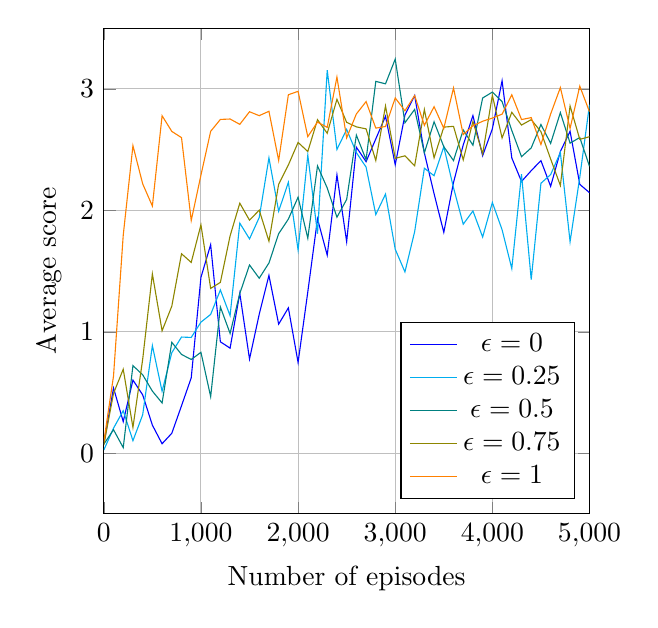
\begin{tikzpicture}
\begin{axis}[height=7.75cm, width=7.75cm, grid=major, xlabel=Number of episodes, ylabel=Average score, xmin=0, xmax=5000, ymin=-0.5, ymax=3.5, legend pos=south east]
\addplot[blue] coordinates {
(0, 0.075783506) (100, 0.5373476) (200, 0.2605691) (300, 0.6018746) (400, 0.4810974) (500, 0.231145) (600, 0.07801781) (700, 0.16424827) (800, 0.3907612) (900, 0.62070036) (1000, 1.448356) (1100, 1.7176728) (1200, 0.91763824) (1300, 0.86524224) (1400, 1.316341) (1500, 0.77580786) (1600, 1.144247) (1700, 1.4641397) (1800, 1.0632023) (1900, 1.1969434) (2000, 0.7473089) (2100, 1.3281183) (2200, 1.9304487) (2300, 1.631062) (2400, 2.2915297) (2500, 1.7418877) (2600, 2.5201461) (2700, 2.400896) (2800, 2.588201) (2900, 2.775009) (3000, 2.3760386) (3100, 2.7850564) (3200, 2.9462454) (3300, 2.4731736) (3400, 2.137) (3500, 1.8188844) (3600, 2.2293358) (3700, 2.538736) (3800, 2.7800798) (3900, 2.4503105) (4000, 2.6716514) (4100, 3.0668533) (4200, 2.43184) (4300, 2.2377641) (4400, 2.326947) (4500, 2.4096606) (4600, 2.1978753) (4700, 2.4844542) (4800, 2.651411) (4900, 2.2142076) (5000, 2.1455436)
};
\addlegendentry{$\epsilon = 0$}

\addplot[cyan] coordinates {
(0, 0.026127584) (100, 0.20603447) (200, 0.3499096) (300, 0.103281155) (400, 0.31549478) (500, 0.8862983) (600, 0.50952387) (700, 0.82788134) (800, 0.9566596) (900, 0.9534169) (1000, 1.0793968) (1100, 1.1429076) (1200, 1.3444846) (1300, 1.1327795) (1400, 1.894753) (1500, 1.7648343) (1600, 1.941155) (1700, 2.4323213) (1800, 1.9930309) (1900, 2.2309103) (2000, 1.6724733) (2100, 2.4551148) (2200, 1.807784) (2300, 3.154453) (2400, 2.501678) (2500, 2.666568) (2600, 2.4754744) (2700, 2.356258) (2800, 1.965614) (2900, 2.133708) (3000, 1.6797562) (3100, 1.4929247) (3200, 1.8244567) (3300, 2.3468375) (3400, 2.2851827) (3500, 2.5243227) (3600, 2.1863897) (3700, 1.8858275) (3800, 1.9951435) (3900, 1.7802545) (4000, 2.0648959) (4100, 1.8405572) (4200, 1.5202707) (4300, 2.297548) (4400, 1.4299351) (4500, 2.2231302) (4600, 2.294632) (4700, 2.4763837) (4800, 1.7417915) (4900, 2.2736173) (5000, 2.8706806)
};
\addlegendentry{$\epsilon = 0.25$}

\addplot[teal] coordinates {
(0, 0.074578114) (100, 0.19332969) (200, 0.04603195) (300, 0.7211557) (400, 0.64624494) (500, 0.5114387) (600, 0.41387236) (700, 0.9134123) (800, 0.8133945) (900, 0.77182984) (1000, 0.83106613) (1100, 0.46566442) (1200, 1.2046154) (1300, 0.9866798) (1400, 1.3154031) (1500, 1.5503093) (1600, 1.4409246) (1700, 1.5665865) (1800, 1.8077103) (1900, 1.9283311) (2000, 2.1081126) (2100, 1.7706008) (2200, 2.3660629) (2300, 2.1842165) (2400, 1.9436227) (2500, 2.0894423) (2600, 2.6194937) (2700, 2.4170773) (2800, 3.0621927) (2900, 3.0420732) (3000, 3.2456293) (3100, 2.7214897) (3200, 2.8314228) (3300, 2.4738798) (3400, 2.7290947) (3500, 2.5242877) (3600, 2.4101129) (3700, 2.6625793) (3800, 2.5361288) (3900, 2.9253216) (4000, 2.973827) (4100, 2.8960137) (4200, 2.6581028) (4300, 2.442151) (4400, 2.5144928) (4500, 2.7068589) (4600, 2.5516794) (4700, 2.8051162) (4800, 2.5536513) (4900, 2.5999148) (5000, 2.3623219)
};
\addlegendentry{$\epsilon = 0.5$}

\addplot[olive] coordinates {
(0, 0.067283146) (100, 0.49277556) (200, 0.6913528) (300, 0.2128624) (400, 0.77164435) (500, 1.4767631) (600, 1.0082191) (700, 1.2108203) (800, 1.6425766) (900, 1.5713556) (1000, 1.881299) (1100, 1.357331) (1200, 1.4068515) (1300, 1.7894717) (1400, 2.0590014) (1500, 1.919088) (1600, 2.001504) (1700, 1.7456108) (1800, 2.2151842) (1900, 2.3738563) (2000, 2.5594602) (2100, 2.484758) (2200, 2.7465868) (2300, 2.6346962) (2400, 2.9149237) (2500, 2.7249253) (2600, 2.6875622) (2700, 2.671085) (2800, 2.4104211) (2900, 2.859832) (3000, 2.4284382) (3100, 2.4490304) (3200, 2.3672037) (3300, 2.8307657) (3400, 2.432613) (3500, 2.6855285) (3600, 2.691947) (3700, 2.4159887) (3800, 2.732229) (3900, 2.464706) (4000, 2.9472816) (4100, 2.5961) (4200, 2.807553) (4300, 2.7026858) (4400, 2.7472079) (4500, 2.6477697) (4600, 2.422682) (4700, 2.2050908) (4800, 2.8598814) (4900, 2.5850205) (5000, 2.6065164)
};
\addlegendentry{$\epsilon = 0.75$}

\addplot[orange] coordinates {
(0, 0.09423332) (100, 0.6353096) (200, 1.7948261) (300, 2.5330555) (400, 2.2189512) (500, 2.0354404) (600, 2.779274) (700, 2.6503074) (800, 2.598851) (900, 1.9162921) (1000, 2.2899916) (1100, 2.6507306) (1200, 2.7487879) (1300, 2.7522595) (1400, 2.7084186) (1500, 2.812137) (1600, 2.7799587) (1700, 2.8159776) (1800, 2.4111073) (1900, 2.9521525) (2000, 2.9802966) (2100, 2.6068614) (2200, 2.726955) (2300, 2.6833677) (2400, 3.0976217) (2500, 2.5968642) (2600, 2.7939558) (2700, 2.895675) (2800, 2.6773908) (2900, 2.6905956) (3000, 2.925931) (3100, 2.820065) (3200, 2.9452431) (3300, 2.700216) (3400, 2.8536344) (3500, 2.675715) (3600, 3.0076885) (3700, 2.623852) (3800, 2.6966531) (3900, 2.7338521) (4000, 2.760093) (4100, 2.7923484) (4200, 2.9515667) (4300, 2.7480175) (4400, 2.7638586) (4500, 2.5421896) (4600, 2.7936602) (4700, 3.0114214) (4800, 2.674845) (4900, 3.0230982) (5000, 2.8112302) 
};
\addlegendentry{$\epsilon = 1$}

\end{axis}
\end{tikzpicture}

&

 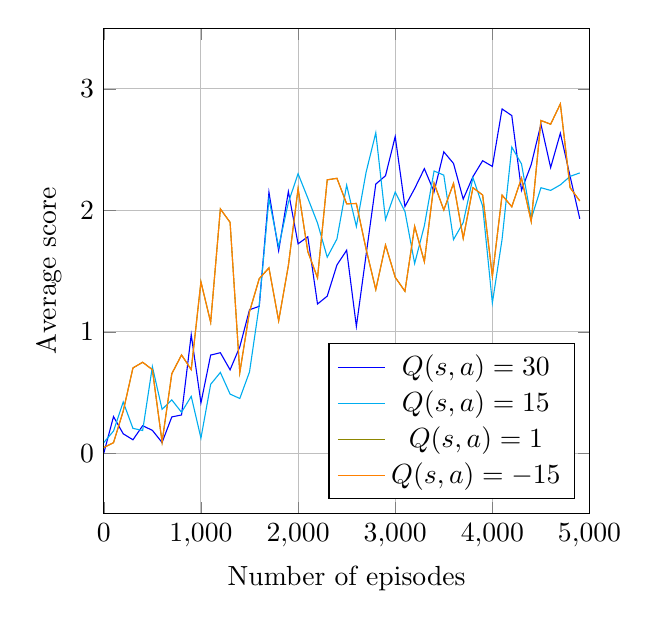
\begin{tikzpicture}
\begin{axis}[height=7.75cm, width=7.75cm, grid=major, xlabel=Number of episodes, ylabel=Average score, xmin=0, xmax=5000, ymin=-0.5, ymax=3.5, legend pos=south east]
\addplot[blue] coordinates {
(0, 2.2149394E-4) (100, 0.30133992) (200, 0.15995665) (300, 0.11061344) (400, 0.22637151) (500, 0.18837589) (600, 0.08820343) (700, 0.29900333) (800, 0.31492093) (900, 0.97605455) (1000, 0.4140383) (1100, 0.80826426) (1200, 0.8276108) (1300, 0.6868575) (1400, 0.8760359) (1500, 1.1812953) (1600, 1.2097125) (1700, 2.1490219) (1800, 1.6686989) (1900, 2.1545887) (2000, 1.7242475) (2100, 1.7825185) (2200, 1.2287631) (2300, 1.2934662) (2400, 1.5501945) (2500, 1.6715132) (2600, 1.0445534) (2700, 1.6334088) (2800, 2.2165613) (2900, 2.2851515) (3000, 2.6077106) (3100, 2.0314047) (3200, 2.1796896) (3300, 2.343577) (3400, 2.1523547) (3500, 2.481914) (3600, 2.38649) (3700, 2.0926511) (3800, 2.2775471) (3900, 2.4086895) (4000, 2.362012) (4100, 2.8351636) (4200, 2.7804465) (4300, 2.165508) (4400, 2.377138) (4500, 2.709607) (4600, 2.3522909) (4700, 2.6354425) (4800, 2.2814956) (4900, 1.9308583)
};
\addlegendentry{$Q(s, a) = 30$}

\addplot[cyan] coordinates {
(0, 0.087629706) (100, 0.18274476) (200, 0.42165244) (300, 0.20467286) (400, 0.18717839) (500, 0.7133571) (600, 0.36128566) (700, 0.43898007) (800, 0.3373194) (900, 0.46822906) (1000, 0.12444008) (1100, 0.56712085) (1200, 0.66531444) (1300, 0.48682228) (1400, 0.4506831) (1500, 0.6696875) (1600, 1.2191303) (1700, 2.0942953) (1800, 1.6980491) (1900, 2.0650263) (2000, 2.3015406) (2100, 2.101208) (2200, 1.8954958) (2300, 1.614249) (2400, 1.7643983) (2500, 2.2072954) (2600, 1.8668244) (2700, 2.313448) (2800, 2.6391096) (2900, 1.9243895) (3000, 2.1511557) (3100, 1.9915051) (3200, 1.5624037) (3300, 1.8738463) (3400, 2.3240974) (3500, 2.2901003) (3600, 1.7591511) (3700, 1.8995636) (3800, 2.2693472) (3900, 2.0353816) (4000, 1.23757) (4100, 1.7619987) (4200, 2.5209537) (4300, 2.3823853) (4400, 1.93071) (4500, 2.1863122) (4600, 2.16428) (4700, 2.2103095) (4800, 2.2798743) (4900, 2.308365)
};
\addlegendentry{$Q(s, a) = 15$}

\addplot[olive] coordinates {
(0, 0.046459362) (100, 0.086777486) (200, 0.34701955) (300, 0.7021876) (400, 0.74912524) (500, 0.6881235) (600, 0.09215304) (700, 0.65425897) (800, 0.80900145) (900, 0.68840134) (1000, 1.4111269) (1100, 1.0782071) (1200, 2.011735) (1300, 1.901412) (1400, 0.6643786) (1500, 1.1655734) (1600, 1.4373999) (1700, 1.5262848) (1800, 1.0903087) (1900, 1.5450555) (2000, 2.1790001) (2100, 1.6609112) (2200, 1.4441974) (2300, 2.2514858) (2400, 2.2640066) (2500, 2.054192) (2600, 2.05643) (2700, 1.6811329) (2800, 1.3473744) (2900, 1.7148299) (3000, 1.4489069) (3100, 1.333591) (3200, 1.868292) (3300, 1.5771114) (3400, 2.223491) (3500, 2.003037) (3600, 2.2220948) (3700, 1.7694572) (3800, 2.1869361) (3900, 2.1263793) (4000, 1.4574677) (4100, 2.12546) (4200, 2.0298264) (4300, 2.2655075) (4400, 1.9079212) (4500, 2.7400007) (4600, 2.7095385) (4700, 2.8769479) (4800, 2.1872087) (4900, 2.0776663)
};
\addlegendentry{$Q(s, a) = 1$}

\addplot[orange] coordinates {
(0, 0.046459362) (100, 0.086777486) (200, 0.34701955) (300, 0.7021876) (400, 0.74912524) (500, 0.6881235) (600, 0.09215304) (700, 0.65425897) (800, 0.80900145) (900, 0.68840134) (1000, 1.4111269) (1100, 1.0782071) (1200, 2.011735) (1300, 1.901412) (1400, 0.6643786) (1500, 1.1655734) (1600, 1.4373999) (1700, 1.5262848) (1800, 1.0903087) (1900, 1.5450555) (2000, 2.1790001) (2100, 1.6609112) (2200, 1.4441974) (2300, 2.2514858) (2400, 2.2640066) (2500, 2.054192) (2600, 2.05643) (2700, 1.6811329) (2800, 1.3473744) (2900, 1.7148299) (3000, 1.4489069) (3100, 1.333591) (3200, 1.868292) (3300, 1.5771114) (3400, 2.223491) (3500, 2.003037) (3600, 2.2220948) (3700, 1.7694572) (3800, 2.1869361) (3900, 2.1263793) (4000, 1.4574677) (4100, 2.12546) (4200, 2.0298264) (4300, 2.2655075) (4400, 1.9079212) (4500, 2.7400007) (4600, 2.7095385) (4700, 2.8769479) (4800, 2.1872087) (4900, 2.0776663)
};
\addlegendentry{$Q(s, a) = -15$}

\end{axis}
\end{tikzpicture}

\end{tabular}

\caption{Performance of the minimax Q-Learning algorithm for different combinations of its parameters. The ``1 predator versus 1 prey'' scenario was tested. Unless otherwise stated, the parameters used were: $\alpha = 0.9, \gamma = 0.9, \epsilon = 0.1, Q(s, a) = 15$.}
\label{fig:minimax-params}
\end{figure}

\newpage

\begin{figure}[ht!]
 \centering
 
 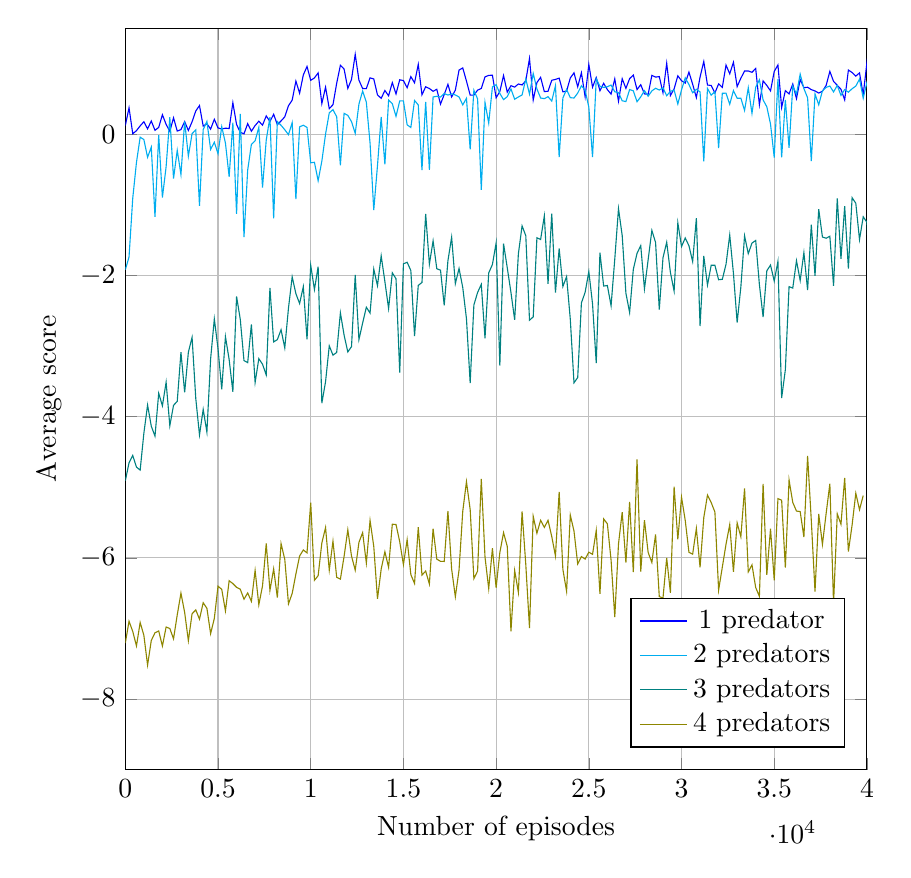
\begin{tikzpicture}
\begin{axis}[height=11cm, width=11cm, grid=major, xlabel=Number of episodes, ylabel=Average score, xmin=0, xmax=40000, ymin=-9, ymax=1.5, legend pos=south east]
\addplot[blue] coordinates {
(0, 0.12311333) (200, 0.37291035) (400, 0.005859607) (600, 0.049466293) (800, 0.11737791) (1000, 0.17613216) (1200, 0.07521633) (1400, 0.18682627) (1600, 0.05445082) (1800, 0.09551313) (2000, 0.27491662) (2200, 0.13851231) (2400, 0.040507913) (2600, 0.23153378) (2800, 0.043900598) (3000, 0.06416984) (3200, 0.17793338) (3400, 0.05202268) (3600, 0.17570023) (3800, 0.32845342) (4000, 0.40452927) (4200, 0.11411854) (4400, 0.14853871) (4600, 0.07157968) (4800, 0.21031915) (5000, 0.08820571) (5200, 0.072937086) (5400, 0.08486481) (5600, 0.07941788) (5800, 0.4452494) (6000, 0.13701701) (6200, 0.025847754) (6400, 0.004841691) (6600, 0.14917505) (6800, 0.04229796) (7000, 0.121590786) (7200, 0.18316235) (7400, 0.12732571) (7600, 0.25809836) (7800, 0.17852926) (8000, 0.28181237) (8200, 0.13457195) (8400, 0.18755656) (8600, 0.24483277) (8800, 0.4035685) (9000, 0.48188838) (9200, 0.7513958) (9400, 0.5798128) (9600, 0.83779556) (9800, 0.9586124) (10000, 0.76200897) (10200, 0.7967857) (10400, 0.86692333) (10600, 0.4330651) (10800, 0.6652868) (11000, 0.3608077) (11200, 0.41720352) (11400, 0.7206782) (11600, 0.9752733) (11800, 0.92140144) (12000, 0.64785194) (12200, 0.7753569) (12400, 1.1302389) (12600, 0.76504636) (12800, 0.6460804) (13000, 0.6453099) (13200, 0.79733175) (13400, 0.7816915) (13600, 0.5568686) (13800, 0.50720525) (14000, 0.6182007) (14200, 0.54308236) (14400, 0.72989583) (14600, 0.5691778) (14800, 0.76986367) (15000, 0.75844496) (15200, 0.6575198) (15400, 0.814738) (15600, 0.72703487) (15800, 0.98957306) (16000, 0.55759645) (16200, 0.67091566) (16400, 0.64596766) (16600, 0.60687184) (16800, 0.63569313) (17000, 0.42546326) (17200, 0.56136364) (17400, 0.70533943) (17600, 0.526573) (17800, 0.62348706) (18000, 0.90752506) (18200, 0.93750405) (18400, 0.7518081) (18600, 0.55356145) (18800, 0.5527333) (19000, 0.6229305) (19200, 0.64682955) (19400, 0.81080806) (19600, 0.83201253) (19800, 0.8350899) (20000, 0.51495993) (20200, 0.60367537) (20400, 0.83035755) (20600, 0.594895) (20800, 0.68623) (21000, 0.6662826) (21200, 0.71033686) (21400, 0.696892) (21600, 0.7549724) (21800, 1.0706741) (22000, 0.48375833) (22200, 0.73100114) (22400, 0.80411315) (22600, 0.60265803) (22800, 0.60719985) (23000, 0.7628744) (23200, 0.7751014) (23400, 0.79276013) (23600, 0.5995053) (23800, 0.60920525) (24000, 0.79524785) (24200, 0.8686073) (24400, 0.67053753) (24600, 0.86897624) (24800, 0.530098) (25000, 0.98808223) (25200, 0.66511005) (25400, 0.80210364) (25600, 0.61496335) (25800, 0.7197734) (26000, 0.6306582) (26200, 0.5673961) (26400, 0.7825887) (26600, 0.46658596) (26800, 0.78488076) (27000, 0.64838743) (27200, 0.7862601) (27400, 0.83730656) (27600, 0.6311794) (27800, 0.70044917) (28000, 0.56972855) (28200, 0.5652089) (28400, 0.83283055) (28600, 0.80763096) (28800, 0.8154031) (29000, 0.58667314) (29200, 1.0039911) (29400, 0.54685885) (29600, 0.64115965) (29800, 0.82638836) (30000, 0.7565814) (30200, 0.72281563) (30400, 0.8781006) (30600, 0.7074866) (30800, 0.51842356) (31000, 0.8090357) (31200, 1.0285946) (31400, 0.6957286) (31600, 0.6890055) (31800, 0.5831901) (32000, 0.71191686) (32200, 0.66293126) (32400, 0.97838193) (32600, 0.85442805) (32800, 1.0186008) (33000, 0.6731355) (33200, 0.7920691) (33400, 0.89382666) (33600, 0.89441955) (33800, 0.875887) (34000, 0.9308016) (34200, 0.41515762) (34400, 0.7541516) (34600, 0.68967533) (34800, 0.6128123) (35000, 0.88829285) (35200, 0.9801734) (35400, 0.37671837) (35600, 0.6159856) (35800, 0.56980926) (36000, 0.7098284) (36200, 0.5036374) (36400, 0.77363306) (36600, 0.65814906) (36800, 0.6641292) (37000, 0.6302255) (37200, 0.6118248) (37400, 0.5816266) (37600, 0.60756665) (37800, 0.6900208) (38000, 0.8891732) (38200, 0.7472557) (38400, 0.6912061) (38600, 0.6355242) (38800, 0.48562765) (39000, 0.9072425) (39200, 0.87221575) (39400, 0.82227844) (39600, 0.8674716) (39800, 0.55969286) (40000, 1.0123445) (40200, 0.5727665) (40400, 0.6666588) (40600, 0.48632938) (40800, 0.44210234) (41000, 0.8067209) (41200, 0.5338333) (41400, 1.0775373) (41600, 1.0583549) (41800, 0.8582168) (42000, 0.6688322) (42200, 0.7719201)
 (42400, 0.6783194) (42600, 0.39015734) (42800, 0.5586302) (43000, 0.60920686) (43200, 0.7198567) (43400, 0.68543106) (43600, 0.88556534) (43800, 0.71035475) (44000, 0.43958923) (44200, 0.71291566) (44400, 0.61034644) (44600, 0.8237655) (44800, 0.7812962) (45000, 0.600354) (45200, 0.64789253) (45400, 0.7088817) (45600, 1.0528073) (45800, 0.6915912) (46000, 0.7195931) (46200, 0.5560597) (46400, 0.89496577) (46600, 0.8038976) (46800, 0.75193614) (47000, 0.7810347) (47200, 1.0323086) (47400, 0.6744882) (47600, 0.65002835) (47800, 0.55864114) (48000, 0.5548241) (48200, 0.79452276) (48400, 0.46607953) (48600, 0.80551004) (48800, 0.9458439) (49000, 0.727809) (49200, 0.8037875) (49400, 0.82720166) (49600, 0.5427888) (49800, 0.5866451)
};
\addlegendentry{1 predator}

\addplot[cyan] coordinates {
(0, -1.9205298) (200, -1.7388507) (400, -0.9073605) (600, -0.40102953) (800, -0.042787094) (1000, -0.07577009) (1200, -0.32746255) (1400, -0.18341602) (1600, -1.170195) (1800, -0.013471894) (2000, -0.8964232) (2200, -0.461334) (2400, 0.24141155) (2600, -0.6283368) (2800, -0.2283712) (3000, -0.57258445) (3200, 0.17929102) (3400, -0.31166205) (3600, 0.007062384) (3800, 0.06026135) (4000, -1.0149127) (4200, 0.06476224) (4400, 0.18024637) (4600, -0.2161829) (4800, -0.11383107) (5000, -0.27707076) (5200, 0.10567677) (5400, -0.12654133) (5600, -0.6028171) (5800, 0.16143693) (6000, -1.1277615) (6200, 0.28646076) (6400, -1.4571576) (6600, -0.50730574) (6800, -0.14445731) (7000, -0.0942236) (7200, 0.09596811) (7400, -0.75506026) (7600, -0.0838999) (7800, 0.2416222) (8000, -1.1905707) (8200, 0.17853034) (8400, 0.12540622) (8600, 0.063145675) (8800, -0.0074097943) (9000, 0.16381152) (9200, -0.92104495) (9400, 0.103478506) (9600, 0.12659189) (9800, 0.09520874) (10000, -0.40493932) (10200, -0.3984471) (10400, -0.6590253) (10600, -0.38123265) (10800, 0.0012456184) (11000, 0.3017538) (11200, 0.34769523) (11400, 0.24596472) (11600, -0.43972054) (11800, 0.29495072) (12000, 0.26569435) (12200, 0.17736508) (12400, 0.011158067) (12600, 0.42560524) (12800, 0.6104738) (13000, 0.4515659) (13200, -0.12716857) (13400, -1.0746186) (13600, -0.44678223) (13800, 0.2442113) (14000, -0.42879558) (14200, 0.48316082) (14400, 0.4319357) (14600, 0.25225952) (14800, 0.47018418) (15000, 0.47148797) (15200, 0.13220464) (15400, 0.09444247) (15600, 0.47647282) (15800, 0.41441393) (16000, -0.5082431) (16200, 0.4579913) (16400, -0.5059505) (16600, 0.526917) (16800, 0.53603107) (17000, 0.5255501) (17200, 0.57500553) (17400, 0.55363375) (17600, 0.5714377) (17800, 0.5549112) (18000, 0.5270285) (18200, 0.41395816) (18400, 0.50761324) (18600, -0.2160332) (18800, 0.62208754) (19000, 0.49980235) (19200, -0.78819203) (19400, 0.44943044) (19600, 0.15605569) (19800, 0.66937125) (20000, 0.7003808) (20200, 0.57675415) (20400, 0.48908287) (20600, 0.5299723) (20800, 0.64070725) (21000, 0.49426118) (21200, 0.5267357) (21400, 0.5551984) (21600, 0.7808315) (21800, 0.56666523) (22000, 0.85946983) (22200, 0.64073783) (22400, 0.5117885) (22600, 0.50305194) (22800, 0.53046525) (23000, 0.46889856) (23200, 0.6858488) (23400, -0.324077) (23600, 0.5122245) (23800, 0.63393724) (24000, 0.51686233) (24200, 0.51145995) (24400, 0.58175015) (24600, 0.68592215) (24800, 0.62283266) (25000, 0.38236663) (25200, -0.324411) (25400, 0.7814563) (25600, 0.67663455) (25800, 0.662174) (26000, 0.6717525) (26200, 0.6951521) (26400, 0.6000952) (26600, 0.58771795) (26800, 0.4727933) (27000, 0.46116132) (27200, 0.631484) (27400, 0.61373323) (27600, 0.45854613) (27800, 0.5283239) (28000, 0.616484) (28200, 0.53675014) (28400, 0.6123955) (28600, 0.64971054) (28800, 0.6250673) (29000, 0.6559675) (29200, 0.54416686) (29400, 0.6062884) (29600, 0.6242639) (29800, 0.42703596) (30000, 0.6278137) (30200, 0.79731476) (30400, 0.7035662) (30600, 0.58567905) (30800, 0.63565135) (31000, 0.59751856) (31200, -0.38559353) (31400, 0.64662665) (31600, 0.55142766) (31800, 0.6020058) (32000, -0.19792818) (32200, 0.57872444) (32400, 0.58086544) (32600, 0.42336738) (32800, 0.616504) (33000, 0.50781614) (33200, 0.5093733) (33400, 0.33630538) (33600, 0.65665066) (33800, 0.29330313) (34000, 0.6629516) (34200, 0.7685369) (34400, 0.48471493) (34600, 0.3877691) (34800, 0.14306435) (35000, -0.33101583) (35200, 0.7795162) (35400, -0.32910508) (35600, 0.48632073) (35800, -0.19368576) (36000, 0.6785098) (36200, 0.56796694) (36400, 0.85033196) (36600, 0.645085) (36800, 0.5149739) (37000, -0.3824525) (37200, 0.56984866) (37400, 0.4154409) (37600, 0.61308813) (37800, 0.66224617) (38000, 0.6818073) (38200, 0.5975949) (38400, 0.68956286) (38600, 0.5483976) (38800, 0.6316321) (39000, 0.59414196) (39200, 0.64343524) (39400, 0.68063575) (39600, 0.77947605) (39800, 0.5099397) (40000, 0.73202765) (40200, 0.6076782) (40400, 0.5504544) (40600, 0.79130054) (40800, 0.5316815) (41000, 0.46923152) (41200, 0.7035572) (41400, 0.45638993) (41600, 0.54590756) (
41800, 0.28495356) (42000, 0.4210467) (42200, 0.5961366) (42400, 0.6309252) (42600, 0.69006634) (42800, 0.53491694) (43000, 0.6315749) (43200, 0.5656968) (43400, 0.6717768) (43600, 0.6573986) (43800, 0.6085026) (44000, 0.5767276) (44200, 0.8486579) (44400, 0.76282483) (44600, 0.4631154) (44800, 0.53580034) (45000, 0.63861525) (45200, 0.57771873) (45400, 0.8456587) (45600, 0.52018434) (45800, 0.58982754) (46000, 0.5666797) (46200, 0.6133327) (46400, 0.48871383) (46600, 0.5242115) (46800, 0.50450265) (47000, 0.5422149) (47200, 0.4639573) (47400, 0.55324805) (47600, 0.5220724) (47800, 0.5162401) (48000, 0.348452) (48200, 0.15957779) (48400, 0.52047724) (48600, 0.4823436) (48800, 0.7674677) (49000, 0.28844145) (49200, 0.6337841) (49400, 0.7250701) (49600, -0.39543876) (49800, 0.50565046)
};
\addlegendentry{2 predators}

\addplot[teal] coordinates {
(0, -4.9071174) (200, -4.652712) (400, -4.5490127) (600, -4.7136345) (800, -4.756412) (1000, -4.233824) (1200, -3.8348536) (1400, -4.13427) (1600, -4.2755885) (1800, -3.6679482) (2000, -3.8464975) (2200, -3.5119019) (2400, -4.128442) (2600, -3.8388453) (2800, -3.7832825) (3000, -3.0877807) (3200, -3.6557941) (3400, -3.0880706) (3600, -2.8769107) (3800, -3.7424674) (4000, -4.2583237) (4200, -3.8963294) (4400, -4.218245) (4600, -3.1834254) (4800, -2.6169224) (5000, -3.0376718) (5200, -3.6137023) (5400, -2.865887) (5600, -3.191361) (5800, -3.646874) (6000, -2.297249) (6200, -2.622241) (6400, -3.2057478) (6600, -3.2344987) (6800, -2.6921887) (7000, -3.5168123) (7200, -3.1788578) (7400, -3.2571013) (7600, -3.4094784) (7800, -2.1770961) (8000, -2.941294) (8200, -2.909035) (8400, -2.7688003) (8600, -3.0264814) (8800, -2.4616702) (9000, -2.0202186) (9200, -2.2590406) (9400, -2.3975222) (9600, -2.159005) (9800, -2.9051096) (10000, -1.8560603) (10200, -2.2001715) (10400, -1.8749034) (10600, -3.8089118) (10800, -3.5042477) (11000, -2.996999) (11200, -3.1289532) (11400, -3.0912564) (11600, -2.5309622) (11800, -2.8461545) (12000, -3.0833483) (12200, -3.0081155) (12400, -1.9938935) (12600, -2.9089007) (12800, -2.6738214) (13000, -2.4502068) (13200, -2.5329614) (13400, -1.9102339) (13600, -2.1451674) (13800, -1.7232242) (14000, -2.0868347) (14200, -2.4689636) (14400, -1.9632053) (14600, -2.0473146) (14800, -3.3743856) (15000, -1.8361404) (15200, -1.8137137) (15400, -1.9307834) (15600, -2.8587127) (15800, -2.1411984) (16000, -2.0997748) (16200, -1.1287754) (16400, -1.8410689) (16600, -1.5103999) (16800, -1.9058323) (17000, -1.9257264) (17200, -2.4227898) (17400, -1.7928406) (17600, -1.4584048) (17800, -2.1166055) (18000, -1.9016328) (18200, -2.1711047) (18400, -2.6133657) (18600, -3.52303) (18800, -2.4185) (19000, -2.2416015) (19200, -2.1267025) (19400, -2.8894951) (19600, -1.9648784) (19800, -1.8453438) (20000, -1.5401996) (20200, -3.2782445) (20400, -1.5489644) (20600, -1.8907325) (20800, -2.2418132) (21000, -2.62964) (21200, -1.6940222) (21400, -1.2985837) (21600, -1.4375904) (21800, -2.6337788) (22000, -2.5875237) (22200, -1.4669489) (22400, -1.4912944) (22600, -1.156166) (22800, -2.117953) (23000, -1.1237682) (23200, -2.24342) (23400, -1.6183263) (23600, -2.1575854) (23800, -2.0176892) (24000, -2.6191342) (24200, -3.5206542) (24400, -3.4452739) (24600, -2.3887262) (24800, -2.2397318) (25000, -1.9455204) (25200, -2.401238) (25400, -3.2416058) (25600, -1.6791135) (25800, -2.150532) (26000, -2.143236) (26200, -2.4293938) (26400, -1.7667283) (26600, -1.0548772) (26800, -1.4354726) (27000, -2.2518468) (27200, -2.5247993) (27400, -1.9133316) (27600, -1.6881315) (27800, -1.5773377) (28000, -2.1906664) (28200, -1.7767869) (28400, -1.3622575) (28600, -1.5332363) (28800, -2.4842696) (29000, -1.7494856) (29200, -1.5298316) (29400, -1.9570346) (29600, -2.2221653) (29800, -1.2547759) (30000, -1.590811) (30200, -1.469945) (30400, -1.5797067) (30600, -1.8043799) (30800, -1.1895766) (31000, -2.715734) (31200, -1.7248567) (31400, -2.1362543) (31600, -1.8556895) (31800, -1.8551278) (32000, -2.0609367) (32200, -2.0554059) (32400, -1.8423837) (32600, -1.4277138) (32800, -1.9705064) (33000, -2.667966) (33200, -2.163207) (33400, -1.4392282) (33600, -1.6916709) (33800, -1.5421077) (34000, -1.5046788) (34200, -2.1302292) (34400, -2.5889962) (34600, -1.934425) (34800, -1.8533816) (35000, -2.0802643) (35200, -1.8006498) (35400, -3.7353756) (35600, -3.3354535) (35800, -2.1589997) (36000, -2.1792288) (36200, -1.7914708) (36400, -2.0717208) (36600, -1.6781937) (36800, -2.2080598) (37000, -1.2826788) (37200, -2.0051293) (37400, -1.0617524) (37600, -1.4563389) (37800, -1.4730577) (38000, -1.4457716) (38200, -2.1478434) (38400, -0.9095116) (38600, -1.7653497) (38800, -1.0205595) (39000, -1.9040694) (39200, -0.8988611) (39400, -0.97899336) (39600, -1.4919605) (39800, -1.1695076) (40000, -1.2484145) (40200, -2.3097048) (40400, -1.4017593) (40600, -0.904639) (40800, -1.2576635) (41000, -1.6474509) (41200, -1.6980352) (41400, -1.4564048) (41600, -1.8576442) (41800, -
1.7595929) (42000, -2.3047762) (42200, -1.9332391) (42400, -2.2392516) (42600, -1.5895427) (42800, -2.0135908) (43000, -2.2242517) (43200, -2.3873806) (43400, -3.1762943) (43600, -1.8211865) (43800, -0.8975095) (44000, -2.6089659) (44200, -1.427368) (44400, -1.9398015) (44600, -1.6506146) (44800, -1.732695) (45000, -2.0061636) (45200, -2.1673157) (45400, -1.5196521) (45600, -1.3748444) (45800, -0.9456674) (46000, -1.8598124) (46200, -1.8355557) (46400, -1.4850588) (46600, -1.7853265) (46800, -1.483574) (47000, -2.8829327) (47200, -2.2321608) (47400, -1.8381963) (47600, -1.7053919) (47800, -2.4133375) (48000, -2.553202) (48200, -2.008681) (48400, -1.7417136) (48600, -1.7222015) (48800, -3.3354173) (49000, -2.0094688) (49200, -2.340471) (49400, -2.2882874) (49600, -2.8248765) (49800, -1.7298245)
};
\addlegendentry{3 predators}

\addplot[olive] coordinates {
(0, -7.204326) (200, -6.895996) (400, -7.0402365) (600, -7.2458105) (800, -6.9141254) (1000, -7.0947) (1200, -7.517242) (1400, -7.1689615) (1600, -7.0589423) (1800, -7.033958) (2000, -7.2464314) (2200, -6.978102) (2400, -6.9990277) (2600, -7.1447377) (2800, -6.8066525) (3000, -6.497849) (3200, -6.7713714) (3400, -7.1716847) (3600, -6.7898445) (3800, -6.735856) (4000, -6.8667536) (4200, -6.6336174) (4400, -6.7121058) (4600, -7.0722866) (4800, -6.856566) (5000, -6.400165) (5200, -6.444447) (5400, -6.749718) (5600, -6.322504) (5800, -6.363051) (6000, -6.415958) (6200, -6.442821) (6400, -6.5842514) (6600, -6.4960127) (6800, -6.61465) (7000, -6.1766963) (7200, -6.6639423) (7400, -6.3955107) (7600, -5.795913) (7800, -6.459772) (8000, -6.1546736) (8200, -6.5625587) (8400, -5.796605) (8600, -6.019558) (8800, -6.6503787) (9000, -6.502327) (9200, -6.2272015) (9400, -5.9725895) (9600, -5.8874416) (9800, -5.9277115) (10000, -5.217822) (10200, -6.3158894) (10400, -6.2511983) (10600, -5.7872834) (10800, -5.5698338) (11000, -6.173165) (11200, -5.7622633) (11400, -6.274094) (11600, -6.2996807) (11800, -5.9775057) (12000, -5.601402) (12200, -5.9736795) (12400, -6.1732626) (12600, -5.779168) (12800, -5.642017) (13000, -6.0727625) (13200, -5.468157) (13400, -5.8350477) (13600, -6.5792904) (13800, -6.157778) (14000, -5.912337) (14200, -6.1329436) (14400, -5.5226536) (14600, -5.5266886) (14800, -5.769714) (15000, -6.0943246) (15200, -5.74182) (15400, -6.2355595) (15600, -6.362314) (15800, -5.564052) (16000, -6.242843) (16200, -6.1858664) (16400, -6.3683476) (16600, -5.5855956) (16800, -6.0170703) (17000, -6.0476556) (17200, -6.049595) (17400, -5.3359265) (17600, -6.157572) (17800, -6.549356) (18000, -6.170373) (18200, -5.339382) (18400, -4.920299) (18600, -5.3141055) (18800, -6.2917943) (19000, -6.1858616) (19200, -4.8825846) (19400, -5.9866405) (19600, -6.435339) (19800, -5.8634105) (20000, -6.4223313) (20200, -5.924627) (20400, -5.642268) (20600, -5.835647) (20800, -7.0385776) (21000, -6.177426) (21200, -6.4870167) (21400, -5.3416905) (21600, -6.0936832) (21800, -6.9929533) (22000, -5.4109063) (22200, -5.6504498) (22400, -5.4665694) (22600, -5.567299) (22800, -5.4677415) (23000, -5.6964474) (23200, -5.971815) (23400, -5.0643806) (23600, -6.1608086) (23800, -6.4715686) (24000, -5.3925853) (24200, -5.6189246) (24400, -6.0856347) (24600, -5.9806094) (24800, -6.015994) (25000, -5.918121) (25200, -5.949048) (25400, -5.6108522) (25600, -6.5080657) (25800, -5.4475126) (26000, -5.5166593) (26200, -6.0306015) (26400, -6.836001) (26600, -5.802559) (26800, -5.351342) (27000, -6.0673857) (27200, -5.2060337) (27400, -6.201626) (27600, -4.6044064) (27800, -6.1944704) (28000, -5.4654408) (28200, -5.9227896) (28400, -6.064593) (28600, -5.665862) (28800, -6.547226) (29000, -6.5672774) (29200, -6.0010085) (29400, -6.4929667) (29600, -4.9915104) (29800, -5.736247) (30000, -5.1400332) (30200, -5.468079) (30400, -5.919684) (30600, -5.945914) (30800, -5.5820894) (31000, -6.1341457) (31200, -5.4296765) (31400, -5.1098185) (31600, -5.2161055) (31800, -5.349407) (32000, -6.454977) (32200, -6.1310887) (32400, -5.805015) (32600, -5.52796) (32800, -6.1961594) (33000, -5.503549) (33200, -5.701496) (33400, -5.016155) (33600, -6.1983657) (33800, -6.0978613) (34000, -6.4185715) (34200, -6.543773) (34400, -4.951609) (34600, -6.2403803) (34800, -5.586165) (35000, -6.3161483) (35200, -5.160545) (35400, -5.1823535) (35600, -6.137922) (35800, -4.895925) (36000, -5.214426) (36200, -5.336201) (36400, -5.343411) (36600, -5.7057147) (36800, -4.5551662) (37000, -5.4700575) (37200, -6.4773703) (37400, -5.3769617) (37600, -5.8085256) (37800, -5.3705153) (38000, -4.948404) (38200, -6.6455784) (38400, -5.3757463) (38600, -5.5230308) (38800, -4.8661904) (39000, -5.9086657) (39200, -5.534749) (39400, -5.0834746) (39600, -5.3167276) (39800, -5.117579)
};
\addlegendentry{4 predators}

\end{axis}
\end{tikzpicture}

\caption{Performance of the independent Q-Learning algorithm for different numbers of predators. In all cases, the parameters used were: $\alpha = 0.9, \gamma = 0.9, \epsilon = 0.1, Q(s, a) = 1$.}
\label{fig:ql-predators}
\end{figure}

\begin{figure}[ht!]
 \centering

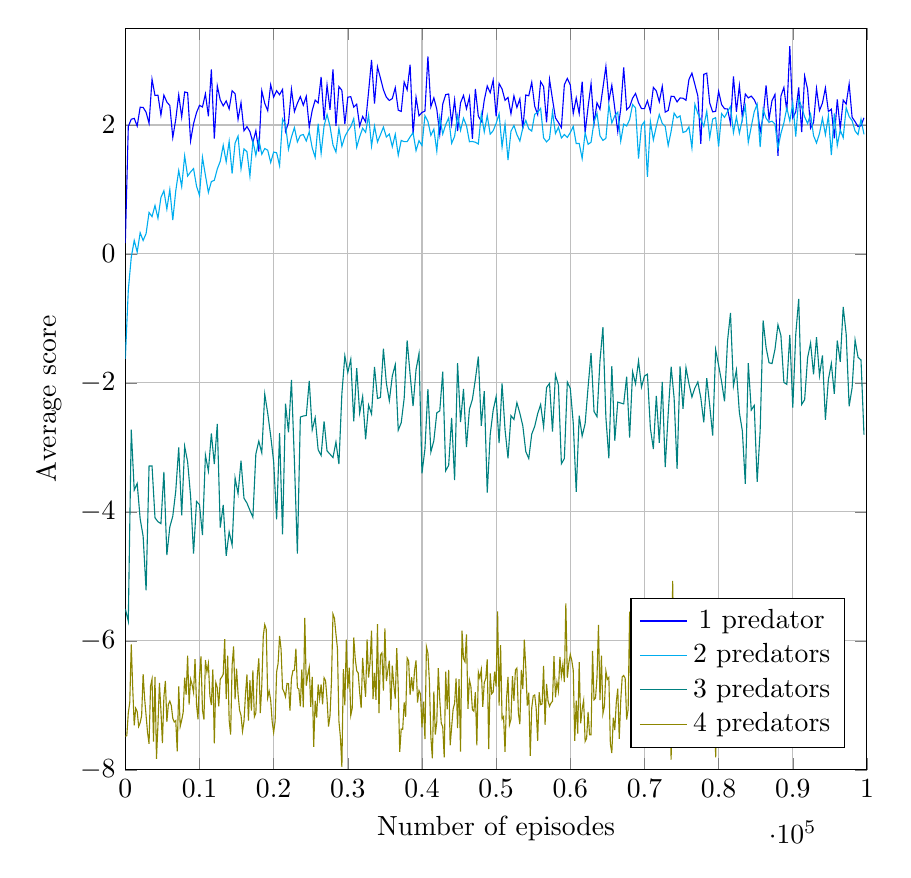
\begin{tikzpicture}
\begin{axis}[height=11cm, width=11cm, grid=major, xlabel=Number of episodes, ylabel=Average score, xmin=0, xmax=100000, ymin=-8, ymax=3.5, legend pos=south east]
\addplot[blue] coordinates {
(0, 0.16920511) (400, 1.9766676) (800, 2.088796) (1200, 2.1020548) (1600, 1.9827542) (2000, 2.2746904) (2400, 2.271511) (2800, 2.1979728) (3200, 2.0247173) (3600, 2.7095475) (4000, 2.4572377) (4400, 2.4617016) (4800, 2.1537654) (5200, 2.462025) (5600, 2.3549528) (6000, 2.3013642) (6400, 1.8053299) (6800, 2.0858593) (7200, 2.4677732) (7600, 2.1222756) (8000, 2.5114472) (8400, 2.4997025) (8800, 1.7545398) (9200, 2.0200927) (9600, 2.1909037) (10000, 2.303992) (10400, 2.2787614) (10800, 2.4820445) (11200, 2.135238) (11600, 2.8599105) (12000, 1.786717) (12400, 2.6064813) (12800, 2.3883212) (13200, 2.295629) (13600, 2.372367) (14000, 2.2485588) (14400, 2.5293941) (14800, 2.4854167) (15200, 2.0863836) (15600, 2.3460336) (16000, 1.9097147) (16400, 1.9735503) (16800, 1.8973777) (17200, 1.7260906) (17600, 1.9099077) (18000, 1.5874639) (18400, 2.5311701) (18800, 2.3355916) (19200, 2.2218578) (19600, 2.6236167) (20000, 2.4319654) (20400, 2.5308275) (20800, 2.4686258) (21200, 2.551325) (21600, 1.8995049) (22000, 2.0329206) (22400, 2.5533679) (22800, 2.2071474) (23200, 2.3356333) (23600, 2.4390283) (24000, 2.306083) (24400, 2.4430234) (24800, 1.965725) (25200, 2.2249932) (25600, 2.385394) (26000, 2.3412435) (26400, 2.744463) (26800, 2.0771594) (27200, 2.6189387) (27600, 2.233161) (28000, 2.8614166) (28400, 1.9849805) (28800, 2.5947475) (29200, 2.5378191) (29600, 2.0148432) (30000, 2.4301813) (30400, 2.4392827) (30800, 2.277186) (31200, 2.320915) (31600, 1.9826343) (32000, 2.1308858) (32400, 2.0470283) (32800, 2.5138204) (33200, 3.009943) (33600, 2.3319843) (34000, 2.901621) (34400, 2.727213) (34800, 2.5457182) (35200, 2.429074) (35600, 2.3803408) (36000, 2.4088204) (36400, 2.5778337) (36800, 2.2299862) (37200, 2.2097008) (37600, 2.6659727) (38000, 2.5446177) (38400, 2.9337063) (38800, 1.8514656) (39200, 2.4288664) (39600, 2.1419418) (40000, 2.1943822) (40400, 2.2137606) (40800, 3.0630212) (41200, 2.2824235) (41600, 2.4218829) (42000, 2.2426906) (42400, 1.8541353) (42800, 2.3236456) (43200, 2.470672) (43600, 2.479773) (44000, 2.0153997) (44400, 2.3882236) (44800, 1.9066124) (45200, 2.342893) (45600, 2.4584577) (46000, 2.251821) (46400, 2.434686) (46800, 1.7861954) (47200, 2.5584447) (47600, 2.1367776) (48000, 2.0562708) (48400, 2.3847327) (48800, 2.6039386) (49200, 2.4999802) (49600, 2.6944718) (50000, 2.1322515) (50400, 2.642565) (50800, 2.557328) (51200, 2.3821676) (51600, 2.4263165) (52000, 2.1731539) (52400, 2.4509132) (52800, 2.27011) (53200, 2.4050765) (53600, 1.9359404) (54000, 2.465085) (54400, 2.4517252) (54800, 2.6613038) (55200, 2.290509) (55600, 2.1615014) (56000, 2.6704202) (56400, 2.5951486) (56800, 2.042022) (57200, 2.7052) (57600, 2.3990595) (58000, 2.1095634) (58400, 2.0379348) (58800, 1.959369) (59200, 2.6249323) (59600, 2.7212129) (60000, 2.619786) (60400, 2.1776316) (60800, 2.4179704) (61200, 2.177219) (61600, 2.6713538) (62000, 1.880399) (62400, 2.2810118) (62800, 2.640202) (63200, 2.019245) (63600, 2.3428402) (64000, 2.2439876) (64400, 2.5744388) (64800, 2.9073517) (65200, 2.3737066) (65600, 2.6170864) (66000, 2.25619) (66400, 1.8965149) (66800, 2.2518854) (67200, 2.8917902) (67600, 2.238103) (68000, 2.2819839) (68400, 2.4149046) (68800, 2.4882522) (69200, 2.3462572) (69600, 2.2530575) (70000, 2.2525158) (70400, 2.3745947) (70800, 2.2064626) (71200, 2.5819988) (71600, 2.5279503) (72000, 2.3594916) (72400, 2.5993032) (72800, 2.1990664) (73200, 2.224335) (73600, 2.4447246) (74000, 2.4410434) (74400, 2.3576746) (74800, 2.4187772) (75200, 2.4143047) (75600, 2.3830922) (76000, 2.7061234) (76400, 2.8033917) (76800, 2.628542) (77200, 2.4479291) (77600, 1.7076519) (78000, 2.784805) (78400, 2.8030474) (78800, 2.339035) (79200, 2.2035894) (79600, 2.210538) (80000, 2.5209954) (80400, 2.3164468) (80800, 2.2517667) (81200, 2.2478647) (81600, 2.0239086) (82000, 2.752134) (82400, 2.2042196) (82800, 2.6103213) (83200, 2.1108556) (83600, 2.479548) (84000, 2.4191852) (84400, 2.4476902) (84800, 2.392043) (85200, 2.2877505) (85600, 1.890017) (86000, 2.1295006) (86400, 2.6127307) (86800, 2.0891192) (87200, 2.3774054) (87600, 2.
4725196) (88000, 1.5224049) (88400, 2.4465303) (88800, 2.582193) (89200, 2.207094) (89600, 3.2222357) (90000, 2.1115313) (90400, 2.203459) (90800, 2.5811884) (91200, 1.8882127) (91600, 2.7580304) (92000, 2.553495) (92400, 1.9486139) (92800, 2.037308) (93200, 2.5639787) (93600, 2.22401) (94000, 2.339635) (94400, 2.5742283) (94800, 2.2082024) (95200, 2.2437906) (95600, 1.794068) (96000, 2.3948383) (96400, 1.937189) (96800, 2.3859758) (97200, 2.323481) (97600, 2.6361818) (98000, 2.1191392) (98400, 2.0511239) (98800, 1.9735801) (99200, 1.9870577) (99600, 2.1110122)
};
\addlegendentry{1 predator}

\addplot[cyan] coordinates {
(0, -1.6270278) (400, -0.56334805) (800, -0.051714014) (1200, 0.20928156) (1600, 0.027931003) (2000, 0.3288187) (2400, 0.20809434) (2800, 0.31617305) (3200, 0.6433456) (3600, 0.5787744) (4000, 0.7508934) (4400, 0.5535617) (4800, 0.87564284) (5200, 0.97933215) (5600, 0.6951346) (6000, 0.99996257) (6400, 0.5259722) (6800, 0.97861177) (7200, 1.2929074) (7600, 1.044233) (8000, 1.5210735) (8400, 1.2075206) (8800, 1.2707875) (9200, 1.3234744) (9600, 1.0509838) (10000, 0.9099587) (10400, 1.4987848) (10800, 1.2196026) (11200, 0.9539759) (11600, 1.1214463) (12000, 1.1418093) (12400, 1.3173229) (12800, 1.4368775) (13200, 1.68432) (13600, 1.4289427) (14000, 1.7442399) (14400, 1.247987) (14800, 1.7186989) (15200, 1.8275963) (15600, 1.3206723) (16000, 1.6282979) (16400, 1.5860597) (16800, 1.2060213) (17200, 1.7530681) (17600, 1.5285208) (18000, 1.7730898) (18400, 1.5460504) (18800, 1.6340735) (19200, 1.6088438) (19600, 1.4177579) (20000, 1.5798072) (20400, 1.568607) (20800, 1.3684661) (21200, 2.093522) (21600, 2.0038865) (22000, 1.6233592) (22400, 1.8124923) (22800, 1.9587291) (23200, 1.7370081) (23600, 1.8384807) (24000, 1.850812) (24400, 1.7516353) (24800, 1.8946189) (25200, 1.6446599) (25600, 1.4983945) (26000, 2.018003) (26400, 1.5608306) (26800, 1.985109) (27200, 2.1636496) (27600, 1.9782708) (28000, 1.6889077) (28400, 1.5799145) (28800, 1.9511349) (29200, 1.6709517) (29600, 1.8174344) (30000, 1.9074496) (30400, 1.9739646) (30800, 2.098198) (31200, 1.6559434) (31600, 1.8178847) (32000, 1.9488415) (32400, 1.885578) (32800, 2.1510804) (33200, 1.6723889) (33600, 1.9834133) (34000, 1.73641) (34400, 1.8493005) (34800, 1.9668677) (35200, 1.8126938) (35600, 1.8572974) (36000, 1.66293) (36400, 1.8552146) (36800, 1.5304142) (37200, 1.760169) (37600, 1.7408928) (38000, 1.7413368) (38400, 1.8149873) (38800, 1.8801455) (39200, 1.6016928) (39600, 1.756214) (40000, 1.6796784) (40400, 2.1443179) (40800, 2.0562108) (41200, 1.8387046) (41600, 1.9360285) (42000, 1.5949538) (42400, 2.120649) (42800, 1.8596222) (43200, 2.0047464) (43600, 2.1085615) (44000, 1.7158322) (44400, 1.822981) (44800, 2.147202) (45200, 1.9163076) (45600, 2.104548) (46000, 1.9907733) (46400, 1.7399161) (46800, 1.7440108) (47200, 1.7315062) (47600, 1.7051047) (48000, 2.173226) (48400, 1.8922161) (48800, 2.1452322) (49200, 1.8573639) (49600, 1.9108509) (50000, 2.0231159) (50400, 2.1736014) (50800, 1.6572635) (51200, 2.0135446) (51600, 1.4561216) (52000, 1.9016528) (52400, 1.9929216) (52800, 1.85124) (53200, 1.7507143) (53600, 1.9545342) (54000, 2.07014) (54400, 1.9400074) (54800, 1.9054242) (55200, 2.164669) (55600, 2.1947727) (56000, 2.2568471) (56400, 1.7983166) (56800, 1.737328) (57200, 1.7866956) (57600, 2.2091968) (58000, 1.8669276) (58400, 1.9632171) (58800, 1.7981479) (59200, 1.8513277) (59600, 1.8073579) (60000, 1.8814919) (60400, 1.9773395) (60800, 1.7101711) (61200, 1.7144971) (61600, 1.4795501) (62000, 1.8771678) (62400, 1.7000079) (62800, 1.7328238) (63200, 2.0516405) (63600, 2.1802742) (64000, 1.8322421) (64400, 1.7604212) (64800, 1.792831) (65200, 2.310735) (65600, 2.0305018) (66000, 2.143312) (66400, 2.1990752) (66800, 1.7479918) (67200, 2.0127852) (67600, 1.9841049) (68000, 2.0826898) (68400, 2.3161952) (68800, 2.2647724) (69200, 1.4779888) (69600, 1.9866986) (70000, 2.0538018) (70400, 1.1954118) (70800, 2.0519888) (71200, 1.7687538) (71600, 1.9781289) (72000, 2.1610346) (72400, 2.024359) (72800, 1.9771069) (73200, 1.680912) (73600, 1.903339) (74000, 2.1838608) (74400, 2.1114712) (74800, 2.140494) (75200, 1.8824109) (75600, 1.9009252) (76000, 1.9704176) (76400, 1.6450397) (76800, 2.318794) (77200, 2.1752956) (77600, 2.0790424) (78000, 1.9787129) (78400, 2.212819) (78800, 1.8036304) (79200, 2.0902617) (79600, 2.113468) (80000, 1.6636832) (80400, 2.1760626) (80800, 2.1174264) (81200, 2.2079704) (81600, 2.2860188) (82000, 1.8816599) (82400, 2.1234412) (82800, 1.8710163) (83200, 2.0924184) (83600, 2.295379) (84000, 1.7299008) (84400, 1.9737823) (84800, 2.2047334) (85200, 2.3224974) (85600, 1.6579831) (86000, 2.2420707) (86400, 2.1039457) (86800, 2.0420427) (87200, 
2.0589795) (87600, 2.0146003) (88000, 1.6397382) (88400, 1.8672345) (88800, 2.0334754) (89200, 2.2651153) (89600, 2.0599494) (90000, 2.3400733) (90400, 1.8213562) (90800, 2.4076872) (91200, 2.273222) (91600, 2.1252244) (92000, 2.0226345) (92400, 2.1692834) (92800, 1.8345816) (93200, 1.7203947) (93600, 1.8676959) (94000, 2.1035035) (94400, 1.850574) (94800, 2.1408606) (95200, 1.5312663) (95600, 2.1770327) (96000, 1.6830544) (96400, 1.9227861) (96800, 1.8028276) (97200, 2.2666311) (97600, 2.128799) (98000, 2.068332) (98400, 1.9064453) (98800, 1.850246) (99200, 2.087442) (99600, 1.8547261)
};
\addlegendentry{2 predators}

\addplot[teal] coordinates {
(0, -5.5044255) (400, -5.693398) (800, -2.725901) (1200, -3.6625977) (1600, -3.559588) (2000, -4.1074905) (2400, -4.376708) (2800, -5.2176943) (3200, -3.28891) (3600, -3.288369) (4000, -4.0916567) (4400, -4.1519303) (4800, -4.182984) (5200, -3.378963) (5600, -4.6712923) (6000, -4.232745) (6400, -4.0661345) (6800, -3.6755445) (7200, -3.0011637) (7600, -4.0553117) (8000, -2.9842238) (8400, -3.2233498) (8800, -3.754681) (9200, -4.647941) (9600, -3.8380783) (10000, -3.8877933) (10400, -4.358563) (10800, -3.1197479) (11200, -3.367117) (11600, -2.7845623) (12000, -3.2574344) (12400, -2.636767) (12800, -4.2429957) (13200, -3.8916967) (13600, -4.6818275) (14000, -4.3093853) (14400, -4.51373) (14800, -3.4733994) (15200, -3.7189918) (15600, -3.2066207) (16000, -3.7881742) (16400, -3.8632488) (16800, -3.9763618) (17200, -4.0820637) (17600, -3.101463) (18000, -2.9028342) (18400, -3.0844316) (18800, -2.174175) (19200, -2.46943) (19600, -2.8200817) (20000, -3.2182117) (20400, -4.117359) (20800, -2.7792306) (21200, -4.346963) (21600, -2.3227959) (22000, -2.7660432) (22400, -1.9522281) (22800, -3.2147338) (23200, -4.646603) (23600, -2.5296068) (24000, -2.5132062) (24400, -2.5055075) (24800, -1.9698528) (25200, -2.728481) (25600, -2.5393357) (26000, -3.0356424) (26400, -3.124318) (26800, -2.5962806) (27200, -3.0543613) (27600, -3.1049783) (28000, -3.1574574) (28400, -2.9162197) (28800, -3.2596738) (29200, -2.1673458) (29600, -1.5800858) (30000, -1.8385259) (30400, -1.6325194) (30800, -2.5966263) (31200, -1.7713226) (31600, -2.4685886) (32000, -2.2107008) (32400, -2.8754349) (32800, -2.3436007) (33200, -2.482664) (33600, -1.751996) (34000, -2.2409577) (34400, -2.225387) (34800, -1.4703653) (35200, -2.005929) (35600, -2.276171) (36000, -1.8920714) (36400, -1.7170727) (36800, -2.733544) (37200, -2.6182709) (37600, -2.2388356) (38000, -1.3427829) (38400, -1.868211) (38800, -2.3602498) (39200, -1.794404) (39600, -1.5441682) (40000, -3.402864) (40400, -3.0247152) (40800, -2.0953324) (41200, -3.071238) (41600, -2.8962305) (42000, -2.464617) (42400, -2.4336486) (42800, -1.8256725) (43200, -3.3617866) (43600, -3.27794) (44000, -2.5416055) (44400, -3.5062299) (44800, -1.6951274) (45200, -2.6056108) (45600, -2.0941236) (46000, -2.9933286) (46400, -2.407376) (46800, -2.25545) (47200, -1.9437848) (47600, -1.5911164) (48000, -2.6657794) (48400, -2.1294732) (48800, -3.7025692) (49200, -2.8028066) (49600, -2.4224136) (50000, -2.2124782) (50400, -2.9334292) (50800, -2.0073388) (51200, -2.7244687) (51600, -3.1710732) (52000, -2.5077608) (52400, -2.5663443) (52800, -2.307179) (53200, -2.4700296) (53600, -2.667373) (54000, -3.0653505) (54400, -3.1718376) (54800, -2.7941654) (55200, -2.673817) (55600, -2.4781044) (56000, -2.3349662) (56400, -2.683002) (56800, -2.07018) (57200, -2.0073469) (57600, -2.7559974) (58000, -1.8721586) (58400, -2.0363579) (58800, -3.2536864) (59200, -3.1729007) (59600, -1.986593) (60000, -2.0854392) (60400, -2.6240551) (60800, -3.6896865) (61200, -2.5070105) (61600, -2.8242986) (62000, -2.6315691) (62400, -2.0634928) (62800, -1.5369458) (63200, -2.443341) (63600, -2.5229876) (64000, -1.6612599) (64400, -1.1351752) (64800, -2.5351496) (65200, -3.1710217) (65600, -1.7396691) (66000, -2.8961859) (66400, -2.2977324) (66800, -2.3114762) (67200, -2.3250828) (67600, -1.9025502) (68000, -2.8476129) (68400, -1.8280137) (68800, -2.0134563) (69200, -1.6582588) (69600, -2.0647666) (70000, -1.8934289) (70400, -1.8641194) (70800, -2.7022676) (71200, -3.024749) (71600, -2.1997054) (72000, -2.92853) (72400, -1.9833984) (72800, -3.306585) (73200, -2.4814074) (73600, -1.7489377) (74000, -2.2355797) (74400, -3.330735) (74800, -1.7457063) (75200, -2.40118) (75600, -1.7629894) (76000, -2.012761) (76400, -2.2185087) (76800, -2.0785897) (77200, -1.9861403) (77600, -2.2334075) (78000, -2.6122818) (78400, -1.9266808) (78800, -2.3484473) (79200, -2.8169875) (79600, -1.4873661) (80000, -1.72621) (80400, -1.9800408) (80800, -2.286755) (81200, -1.3509773) (81600, -0.914884) (82000, -2.0468528) (82400, -1.800249) (82800, -2.4601486) (83200, -2.744667) (83600, -
3.5657945) (84000, -1.6934695) (84400, -2.4224312) (84800, -2.349578) (85200, -3.5347292) (85600, -2.7395282) (86000, -1.0310025) (86400, -1.4505745) (86800, -1.6872754) (87200, -1.7005478) (87600, -1.4784814) (88000, -1.0971056) (88400, -1.2637897) (88800, -1.9913838) (89200, -2.0229614) (89600, -1.2548438) (90000, -2.3829274) (90400, -1.2486967) (90800, -0.6963836) (91200, -2.333852) (91600, -2.2603636) (92000, -1.6091977) (92400, -1.3822091) (92800, -1.8673544) (93200, -1.2905972) (93600, -1.8875531) (94000, -1.572799) (94400, -2.5712397) (94800, -1.9479184) (95200, -1.6993059) (95600, -2.170168) (96000, -1.3433305) (96400, -1.6732882) (96800, -0.8214491) (97200, -1.2407119) (97600, -2.3627062) (98000, -2.0739417) (98400, -1.333363) (98800, -1.603207) (99200, -1.6444278) (99600, -2.8030844)
};
\addlegendentry{3 predators}

\addplot[olive] coordinates {
(0, -7.4783616) (200, -7.470609) (400, -7.1180353) (600, -6.9569774) (800, -6.0564537) (1000, -6.739993) (1200, -7.308371) (1400, -7.0449305) (1600, -7.0951414) (1800, -7.327576) (2000, -7.2708135) (2200, -7.1588287) (2400, -6.514673) (2600, -6.891074) (2800, -7.1584215) (3000, -7.4248033) (3200, -7.59569) (3400, -6.7033386) (3600, -6.593089) (3800, -7.5611176) (4000, -6.5572796) (4200, -7.8283663) (4400, -7.3002973) (4600, -6.6531224) (4800, -7.0787263) (5000, -7.5846562) (5200, -6.8706994) (5400, -6.6207886) (5600, -7.254834) (5800, -6.9866753) (6000, -6.934123) (6200, -7.002594) (6400, -7.2011824) (6600, -7.2573795) (6800, -7.2367177) (7000, -7.713604) (7200, -6.7041993) (7400, -7.326567) (7600, -7.2298145) (7800, -7.107818) (8000, -6.571755) (8200, -6.8375816) (8400, -6.2294765) (8600, -6.986358) (8800, -6.5958734) (9000, -6.6761866) (9200, -6.7995367) (9400, -6.28396) (9600, -6.985945) (9800, -7.2148833) (10000, -6.557257) (10200, -6.240183) (10400, -7.069107) (10600, -7.2193575) (10800, -6.2972856) (11000, -6.4813886) (11200, -6.3519044) (11400, -6.8497286) (11600, -6.9942436) (11800, -6.4408484) (12000, -7.5889306) (12200, -6.645133) (12400, -6.726632) (12600, -7.015425) (12800, -6.593308) (13000, -6.562053) (13200, -6.5174565) (13400, -5.9743223) (13600, -6.904136) (13800, -6.2281303) (14000, -7.230722) (14200, -7.451652) (14400, -6.3762374) (14600, -6.087492) (14800, -6.908129) (15000, -6.431926) (15200, -6.8192034) (15400, -7.0719867) (15600, -7.1549444) (15800, -7.4020915) (16000, -7.24721) (16200, -6.831602) (16400, -6.521873) (16600, -7.2377977) (16800, -6.6101265) (17000, -7.0793724) (17200, -6.4592423) (17400, -7.177567) (17600, -7.1178594) (17800, -6.5386796) (18000, -6.270198) (18200, -7.1196995) (18400, -6.697472) (18600, -5.9260073) (18800, -5.7469997) (19000, -5.8198853) (19200, -6.8804545) (19400, -6.781526) (19600, -6.9185357) (19800, -7.2512803) (20000, -7.4202375) (20200, -7.2439146) (20400, -6.4815464) (20600, -6.3486423) (20800, -5.921604) (21000, -6.1278577) (21200, -6.7430534) (21400, -6.790661) (21600, -6.866259) (21800, -6.660078) (22000, -6.664419) (22200, -7.082977) (22400, -6.5827174) (22600, -6.461895) (22800, -6.4542985) (23000, -6.119306) (23200, -6.727798) (23400, -6.7465596) (23600, -7.0167065) (23800, -6.4426384) (24000, -7.0326924) (24200, -5.641962) (24400, -6.6948986) (24600, -6.5275702) (24800, -6.4081316) (25000, -7.022594) (25200, -6.5569005) (25400, -7.643439) (25600, -6.9290676) (25800, -7.190933) (26000, -6.676801) (26200, -6.8946905) (26400, -6.674696) (26600, -6.983571) (26800, -6.5720754) (27000, -6.620244) (27200, -6.905304) (27400, -7.3289375) (27600, -7.159737) (27800, -6.6168194) (28000, -5.5853224) (28200, -5.650643) (28400, -5.8957324) (28600, -6.1139684) (28800, -7.242308) (29000, -7.4930816) (29200, -7.954695) (29400, -6.4386888) (29600, -7.001701) (29800, -5.9804106) (30000, -6.7399907) (30200, -6.4148216) (30400, -7.155601) (30600, -7.040021) (30800, -5.948076) (31000, -6.2744484) (31200, -6.4634852) (31400, -6.4973407) (31600, -6.801208) (31800, -7.0409765) (32000, -6.2622204) (32200, -6.6071224) (32400, -6.865999) (32600, -5.977981) (32800, -6.570755) (33000, -6.3367643) (33200, -5.8406324) (33400, -6.9041333) (33600, -6.4978833) (33800, -6.913673) (34000, -5.7412457) (34200, -7.1215405) (34400, -6.218115) (34600, -6.1851606) (34800, -6.7729735) (35000, -5.806691) (35200, -6.62408) (35400, -6.454207) (35600, -6.3056417) (35800, -7.0721564) (36000, -6.384254) (36200, -6.683399) (36400, -6.893385) (36600, -6.114058) (36800, -6.7418256) (37000, -7.722231) (37200, -7.366856) (37400, -7.3726) (37600, -6.9542456) (37800, -7.176533) (38000, -6.2646804) (38200, -6.3086576) (38400, -6.835562) (38600, -6.5624905) (38800, -6.7829475) (39000, -6.4595923) (39200, -6.3019385) (39400, -6.955299) (39600, -6.7702913) (39800, -6.821411) (40000, -7.3398204) (40200, -6.941683) (40400, -7.5247912) (40600, -6.089777) (40800, -6.1874943) (41000, -6.623838) (41200, -7.4943585) (41400, -7.8221607) (41600, -6.7852507) (41800, -7.4529657) (42000, -7.2511296) (42200, -6.4240446) (42400,
 -6.916175) (42600, -7.273834) (42800, -7.33571) (43000, -7.806409) (43200, -6.4762807) (43400, -7.0602193) (43600, -6.449788) (43800, -7.6208) (44000, -7.3379407) (44200, -7.056749) (44400, -6.9695697) (44600, -6.5812416) (44800, -7.352302) (45000, -6.5949574) (45200, -7.7157135) (45400, -5.841217) (45600, -6.275047) (45800, -6.325734) (46000, -5.9013696) (46200, -7.052477) (46400, -6.608545) (46600, -6.710009) (46800, -7.0663147) (47000, -7.091786) (47200, -6.7936225) (47400, -7.6203923) (47600, -6.4836354) (47800, -6.5767717) (48000, -6.4466496) (48200, -7.0222816) (48400, -6.6478386) (48600, -6.582663) (48800, -6.2869854) (49000, -7.679275) (49200, -6.503687) (49400, -6.8203173) (49600, -6.7943664) (49800, -6.476106) (50000, -6.7083216) (50200, -5.5442114) (50400, -7.003459) (50600, -6.064352) (50800, -7.2117524) (51000, -7.1756563) (51200, -7.721189) (51400, -6.905542) (51600, -6.557764) (51800, -7.301316) (52000, -7.214063) (52200, -6.545818) (52400, -6.929999) (52600, -6.4506373) (52800, -6.421757) (53000, -7.1205034) (53200, -7.2919784) (53400, -6.4491563) (53600, -6.746904) (53800, -5.9825964) (54000, -6.4177785) (54200, -7.0032377) (54400, -6.8017645) (54600, -7.7825747) (54800, -7.040139) (55000, -6.8546576) (55200, -6.839039) (55400, -7.045706) (55600, -7.551654) (55800, -6.795619) (56000, -6.9891872) (56200, -6.9791145) (56400, -6.3864303) (56600, -7.30217) (56800, -6.6677566) (57000, -6.9320817) (57200, -7.0151525) (57400, -6.9639897) (57600, -6.9370623) (57800, -6.2372255) (58000, -6.875964) (58200, -6.639192) (58400, -6.776278) (58600, -6.24767) (58800, -6.544985) (59000, -6.3673573) (59200, -6.637672) (59400, -5.4184523) (59600, -6.571076) (59800, -6.344892) (60000, -6.210291) (60200, -6.3043346) (60400, -6.457216) (60600, -7.54872) (60800, -6.9282517) (61000, -7.438802) (61200, -6.328456) (61400, -7.277688) (61600, -7.0615587) (61800, -6.9242187) (62000, -7.5594893) (62200, -7.5114064) (62400, -7.103334) (62600, -7.455283) (62800, -7.4566665) (63000, -6.156175) (63200, -6.9123735) (63400, -6.8884473) (63600, -6.5649757) (63800, -5.7536025) (64000, -6.9179745) (64200, -6.2302413) (64400, -7.12892) (64600, -7.016227) (64800, -6.4686265) (65000, -6.597216) (65200, -6.566629) (65400, -7.5916457) (65600, -7.7388396) (65800, -7.1899257) (66000, -7.3836226) (66200, -6.9562383) (66400, -6.7400208) (66600, -7.5192633) (66800, -6.9321046) (67000, -6.5587044) (67200, -6.5375934) (67400, -6.5800323) (67600, -7.2198424) (67800, -7.0625696) (68000, -5.5452385) (68200, -7.1396675) (68400, -7.3969707) (68600, -6.7174873) (68800, -6.940264) (69000, -6.0471954) (69200, -6.0205107) (69400, -5.785671) (69600, -6.326225) (69800, -6.357804) (70000, -5.7598352) (70200, -5.9036226) (70400, -6.8099422) (70600, -6.9736347) (70800, -5.936375) (71000, -6.4361577) (71200, -6.3835225) (71400, -6.02258) (71600, -6.7421703) (71800, -6.3517485) (72000, -6.972129) (72200, -6.704064) (72400, -6.339612) (72600, -6.0775776) (72800, -6.5872865) (73000, -6.7930126) (73200, -6.954505) (73400, -7.056045) (73600, -7.843107) (73800, -5.0689) (74000, -6.3281846) (74200, -6.2524657) (74400, -5.719424) (74600, -5.927682) (74800, -6.4861813) (75000, -6.293379) (75200, -5.6678233) (75400, -5.8876495) (75600, -7.27844) (75800, -6.3624744) (76000, -6.9041805) (76200, -7.0022316) (76400, -6.864882) (76600, -6.5378175) (76800, -6.8767114) (77000, -7.390922) (77200, -6.6933312) (77400, -6.17591) (77600, -6.6724195) (77800, -6.672256) (78000, -6.930402) (78200, -6.8363357) (78400, -6.8662806) (78600, -7.431753) (78800, -6.202187) (79000, -6.9123864) (79200, -5.7123675) (79400, -6.5899076) (79600, -7.8081183) (79800, -7.075613) (80000, -7.6008797) (80200, -7.0989285) (80400, -7.3433924) (80600, -6.813019) (80800, -7.0353394) (81000, -6.6040745) (81200, -5.5232415) (81400, -7.025585) (81600, -7.070279) (81800, -6.494102) (82000, -6.7903996) (82200, -6.623032) (82400, -6.605455) (82600, -6.8016295) (82800, -6.888717) (83000, -6.5463753) (83200, -6.9942937) (83400, -6.0896916) (83600, -6.208919) (83800, -6.3217745) (84000, -7.2036324) (84200, -6.489076) (
84400, -6.614531) (84600, -6.997522) (84800, -6.8716145) (85000, -6.604211) (85200, -5.899142) (85400, -6.5976753) (85600, -6.232178) (85800, -6.7167964) (86000, -6.879657) (86200, -6.6479774) (86400, -6.441603) (86600, -6.3512616) (86800, -6.166059) (87000, -6.6221075) (87200, -6.6811695) (87400, -6.0221868) (87600, -6.4281) (87800, -6.1931334) (88000, -6.8877397) (88200, -6.2000165) (88400, -6.5655694) (88600, -6.625068) (88800, -6.987784) (89000, -6.5014668) (89200, -6.040895) (89400, -6.147367) (89600, -7.0747294) (89800, -6.3320727) (90000, -6.847543) (90200, -6.6996355) (90400, -6.6729803) (90600, -6.730753) (90800, -6.716782) (91000, -6.764394) (91200, -7.2502418) (91400, -6.353304) (91600, -5.673509) (91800, -6.586166) (92000, -5.6575313) (92200, -6.3214703) (92400, -7.022624)
};
\addlegendentry{4 predators}

\end{axis}
\end{tikzpicture}

\caption{Performance of the GIGA-WoLF algorithm for different numbers of predators. In all cases, the parameters used were: $\gamma = 0.9, \eta = 0.1$.}
\label{fig:wolf-predators}
\end{figure}

\newpage

\section{Discussion}

\subsection{Independent Q-Learning}

We will first comment the different behaviours of the algorithm when using different parameter settings on the ``1 predator versus 1 prey'' scenario. Our results are summarized in figure \ref{fig:ql-params}. We will also compare these results with those we obtained for the stardard Q-Learning algorithm we implemented for the previous assignment.

First of all, we can see how different values of $\gamma$ yield very different solutions. With $\gamma = 0$ the agents do not look into the future at all and the performance is the worst of all: around 0.2 ($T \approx 38.1 $). This is the expected result. However, and more surprisingly, intermediate values of $\gamma$ seem to perform better than high ones: we got averages scores of around 1.25 ($T \approx 20.7 $) for $\gamma = 0.3$ and $\gamma = 0.6$ but scores around 0.75 ($T \approx 25.6 $) for $\gamma = 0.9$. These results are different from those we got for the standard Q-Learning version, where we found that higher values of $\gamma$ always improved the solutions found.

The behaviour shown for different values of the parameter $\alpha$ is similar to the previous case. Extreme values give the worst results, while more intermediate ones perform better. We obtained scores around 0.6 ($ T \approx 27.7 $) for $\alpha = 0.1$ and $\alpha = 1$, and scores around 1.75 ($ T \approx 17.5 $) for $\alpha = 0.4$ and $\alpha = 0.7$. It is also worth mentioning how the algorithm experiences a sudden improvement on performance at a given threshold for the number of episodes generated. The location of this point seems to depend on the choice of the parameter itself. This can be observed across most cases we studied in figure \ref{fig:ql-params}. Finally, these results are different from those we got for the standard Q-Learning version, where we found that higher values of $\alpha$ always improved the solutions found.

Different values of the parameter $\epsilon$ also show similar behaviours to the previous cases. The best results are obtained with a completely greedy policy ($\epsilon = 0$), which obtains a remarkably good score, around 2 ($T = 16.3 $). This case also looks the most stable, since less noice is noticeable in the plot when compared to the rest of cases. Higher values of $\epsilon$ yield worse results, with $\epsilon = 1$ performing slightly better than the rest. These results are completely opposite to those we got for the standard Q-Learning version, where we found that higher values of $\epsilon$ always improved the solutions found.

Finally, the initial values for the $Q$ table also play a major role in the performance of the algorithm. We can see in the figure how optimistic initializations perform, on average, worse than their pessimistic counterparts. The behaviours for the optimistic values $Q(s, a) = 30 $ and $Q(s, a) = 15 $ are identical. $Q(s, a) = 0 $ shows a faster convergence than $Q(s, a) = -15 $, most likely due to the fact that the latter is a worse estimator of the true value of the $Q$ table than the first one.

We will now comment on the performance of the algorithm when considering different numbers of predators, while keeping the rest of the parameters fixed. Our results are summarized in figure \ref{fig:ql-predators}. Firstly, it is surprising that the solutions become worse the higher the number of predators is. We would expect that having more predators should help in the task of catching the prey more quickly, since the predators could coordinate to surround the prey. For 1 and 2 predators, the solutions found by the algorithm manage to catch the prey quicker on average ($ T \approx 22.9 $) than the predators take to collide into each other. This is not the case for 3 (final score around -1, $ T \approx 22.9 $) and 4 predators (final score around -5, $ T \approx 7.6 $). The more predators we add, the sooner they will collide into each other. This suggests that the state-space is too large for the algorithm to find good solutions to the problem in those cases in a reasonable amount of time. We can see how the performance steadily and slowly increases for the cases of 3 and 4 predators, but we were not able to generate more episodes for these due to the lack of memory of the computing system we used to perform our experiments.

\subsection{Minimax Q-Learning}

We will now comment on the performance of the Minimax Q-Learning algorithm based on the results we obtained in our tests. These results are summarized in in figure \ref{fig:minimax-params}. 

In the first plot we can see how the performance is influenced by the value of $\gamma$. For $\gamma= 0.3$ we have an initial increase in performance and a slow decrease after about 3500 episodes, while for $gamma = 0.6$ and $gamma=0.9$ we have similar results. For those values of gamma the performance seems to be always increasing, and for $gamma = 0.6$ a peak of 3.17 ($ T \approx 12 $ ) is reached.

For different values of $\alpha$ we have quite similar results, and the performance seems to be still increasing after 5000 episodes.
Even if the results are similar, with $\alpha = 1$ performance is a bit worse as expected, and middle values such as  $\alpha = 0.4$ and $\alpha = 0.7$ lead to the best results. 

From the results we show in plot 3, we can see how with $\epsilon = 0$ we covergence is reached in a lower number of episodes then for the other values of $\epsilon$. The convergence value is then similar for all the values of $\epsilon$. We have to consider however that episodesed generated using the random policy (defined by $epsilon = 1$) tend to last more than episodes generated with a soft policy, so less number of episodes don't necessarily equal to lower time. 

We can then evaluate the test results for different values of inizialization of the Q-table. We can see how for optimistic values of Q(s,a) such as Q(s,a)=15 and Q(s,a)=30 give similar result as for Q(s,a)=1.


\subsection{Q-learning vs Minimax Q-learning}
Given the data we have obtained, we can only compare the performance of the two algorithms for a running period of 5000 episodes. However we can already see how Minimax converges in fewer steps and reaches higher peaks of performance. Also the various parameters affect less the performance in Minimax, while in Q-learning all the parameters have a visible influence on the outcome of the algorithm.

\subsection{GIGA-WoLF}

We will comment on the performance of the algorithm when considering different numbers of predators, while keeping the rest of the parameters fixed. Our results are summarized in figure \ref{fig:wolf-predators}. We will also compare these results with those we obtained for the independent Q-Learning algorithm.

We can again notice how the solutions become worse the higher the number of predators is, just as it was the case with Q-Learning. However, the performance is different for each case. For 1 and 2 predators, the solutions found by GIGA-WoLF are better than those of independent Q-Learning: they archieve scores of 2 ($T = 16.3 $) versus 0.5 ($T = 29.4$), respectively. For the case of 3 predators, no differences can be appreciated between both algorithms. However, in the 4 predators scenario, GIGA-WoLF is surprisingly unable to make any improvement to the solutions found, while Q-Learning is still able to slowly improve the average score.

\section{Conclusion}

We have implemented and studied the performance of the independent Q-Learning algorithm, the minimax Q-Learning algorithm, and a model-free, multi-timestep version of the GIGA-WoLF algorithm. We also derived a score system and a reduced state-space encoding suitable for the multi-predator scenario. We can summarize our main conclusions from this assignment as follows:

\begin{itemize}
 \item The best solution for the 1 predator scenario was found by the minimax Q-Learning algorithm ($ T \approx 12 $).
 \item The independent Q-Learning algorithm manages to find good quality solutions for the scenarios with 1 and 2 predators.
 \item All solutions found for the cases having 3 or 4 predators did not manage to catch the prey quicker and/or more often than it takes the predators to collide into each other.
 \item Choices of intermediate values for the parameters $\gamma$ and $\alpha$ seem to improve the convergence rate of independent Q-Learning. We obtained the best performance using $\epsilon = 0$. An initialization of the values of the $Q$ table to 0 was found to yield the best results.
 \item The GIGA-WoLF algorithm manages to improve the solutions found by independent Q-Learning for the cases with 1 and 2 predators, it yields similar results for 3 predators, and it does not work with 4 predators.
 \item The huge state-space that results from having more than 2 predators seriously limits the applicability and usefulness of the algorithms we implemented for this assignment. 
\end{itemize}

\thebibliography{}
%\url{http://www.wikibooks.org}
%\href{http://www.wikibooks.org}{Wikibooks home}
\bibitem{Assignment}
  \emph{Assignment}.\\
  Assignments Autonomous Agents, D.M Roijers, September 2, 2013 \\

\bibitem{vlasis}  
	\emph{Vlassis Nicos} \\
	A Concise Introduction to Multiagent Systems and Distributed Artificial Intelligence \\
	Morgan and Claypool Publishers, 2007 \\

\bibitem{SB}
  \emph{Sutton and Barto}.\\
  Reinforcement Learning: An Introduction, Richard S. Sutton, Andrew G Barto. \\
  \url{http://webdocs.cs.ualberta.ca/~sutton/book/ebook/} \\
 
 \bibitem{minimax}
 Michael L. Littman \\
 Markov games as a framework for multi-agent reinforcement learning \\
 Brown University / Bellcore, 1994 \\
 \url{http://www.cs.rutgers.edu/~mlittman/papers/refer.html} \\
 
 \bibitem{hk}
 Lecture notes from: \\ 
 Topics in Algorithms: Combinatorial Optimization and Approximation Algorithms \\
 The Chinese University of Hong Kong \\
 Lecture 14 \\
 \url{http://appsrv.cse.cuhk.edu.hk/~chi/csc5160-2008/notes.html} \\
 
 \bibitem{GIGA-wolf}
 Michael Bowling \\
 Convergence and no-regret in Multiagent Learning, 2004 \\
 \url{http://webdocs.cs.ualberta.ca/~bowling/papers/04nips.pdf}

\bibitem{PHC}
 Bowling and Veloso, \\
 Rational and Convergent Learning in Stochastic Games, (2001) \\
\url{http://www.cs.cmu.edu/~mmv/papers/01ijcai-mike.pdf}
\end{document}
